
Here I show the full table for \autoref{fig:nn_comp}.

\begin{tiny}
\begin{longtable}{p{2.5cm}||cccc}
  \hline \\
  & Neural network - 26 & SVM - polynomial & Neural network 5+3 & SVM - radial \\
  \hline \\ \endhead
  &
    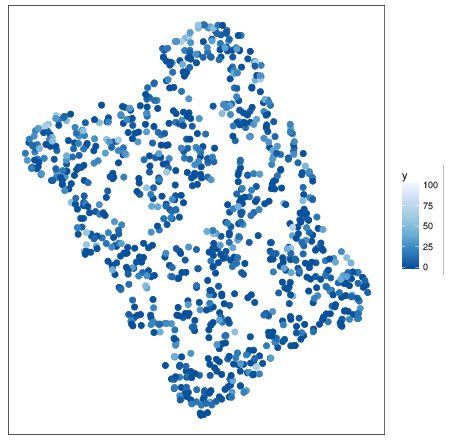
\includegraphics[width=0.1\textwidth]{boston_nn_26_sp.png}
  &
    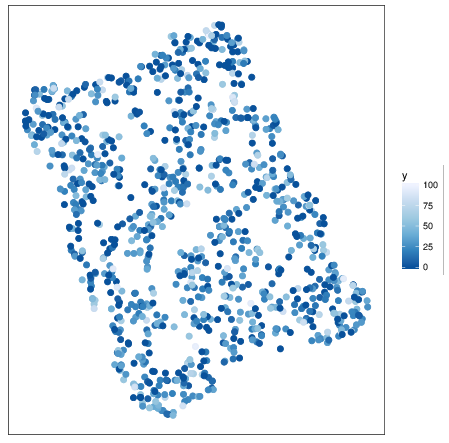
\includegraphics[width=0.1\textwidth]{boston_svm_poly_sp.png}
  &
    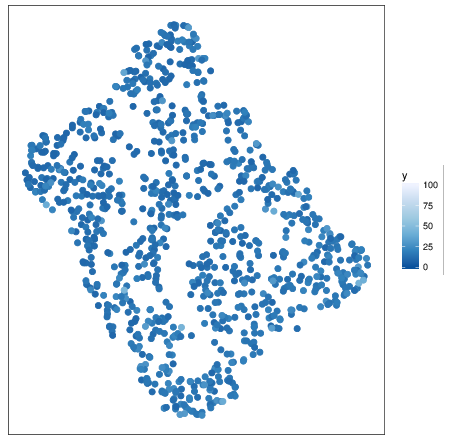
\includegraphics[width=0.1\textwidth]{boston_nn_5x3_sp.png}
  &
    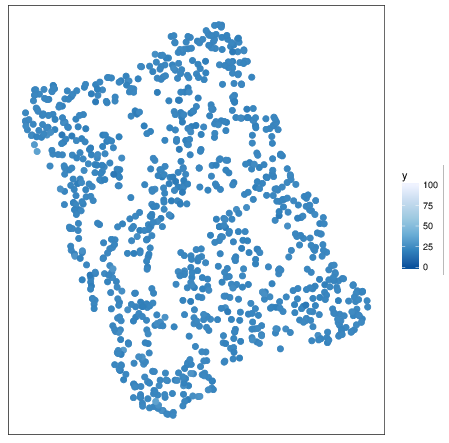
\includegraphics[width=0.1\textwidth]{boston_svm_radial_sp.png}
  \\
  \hline \\
  Per capita crime rate &
    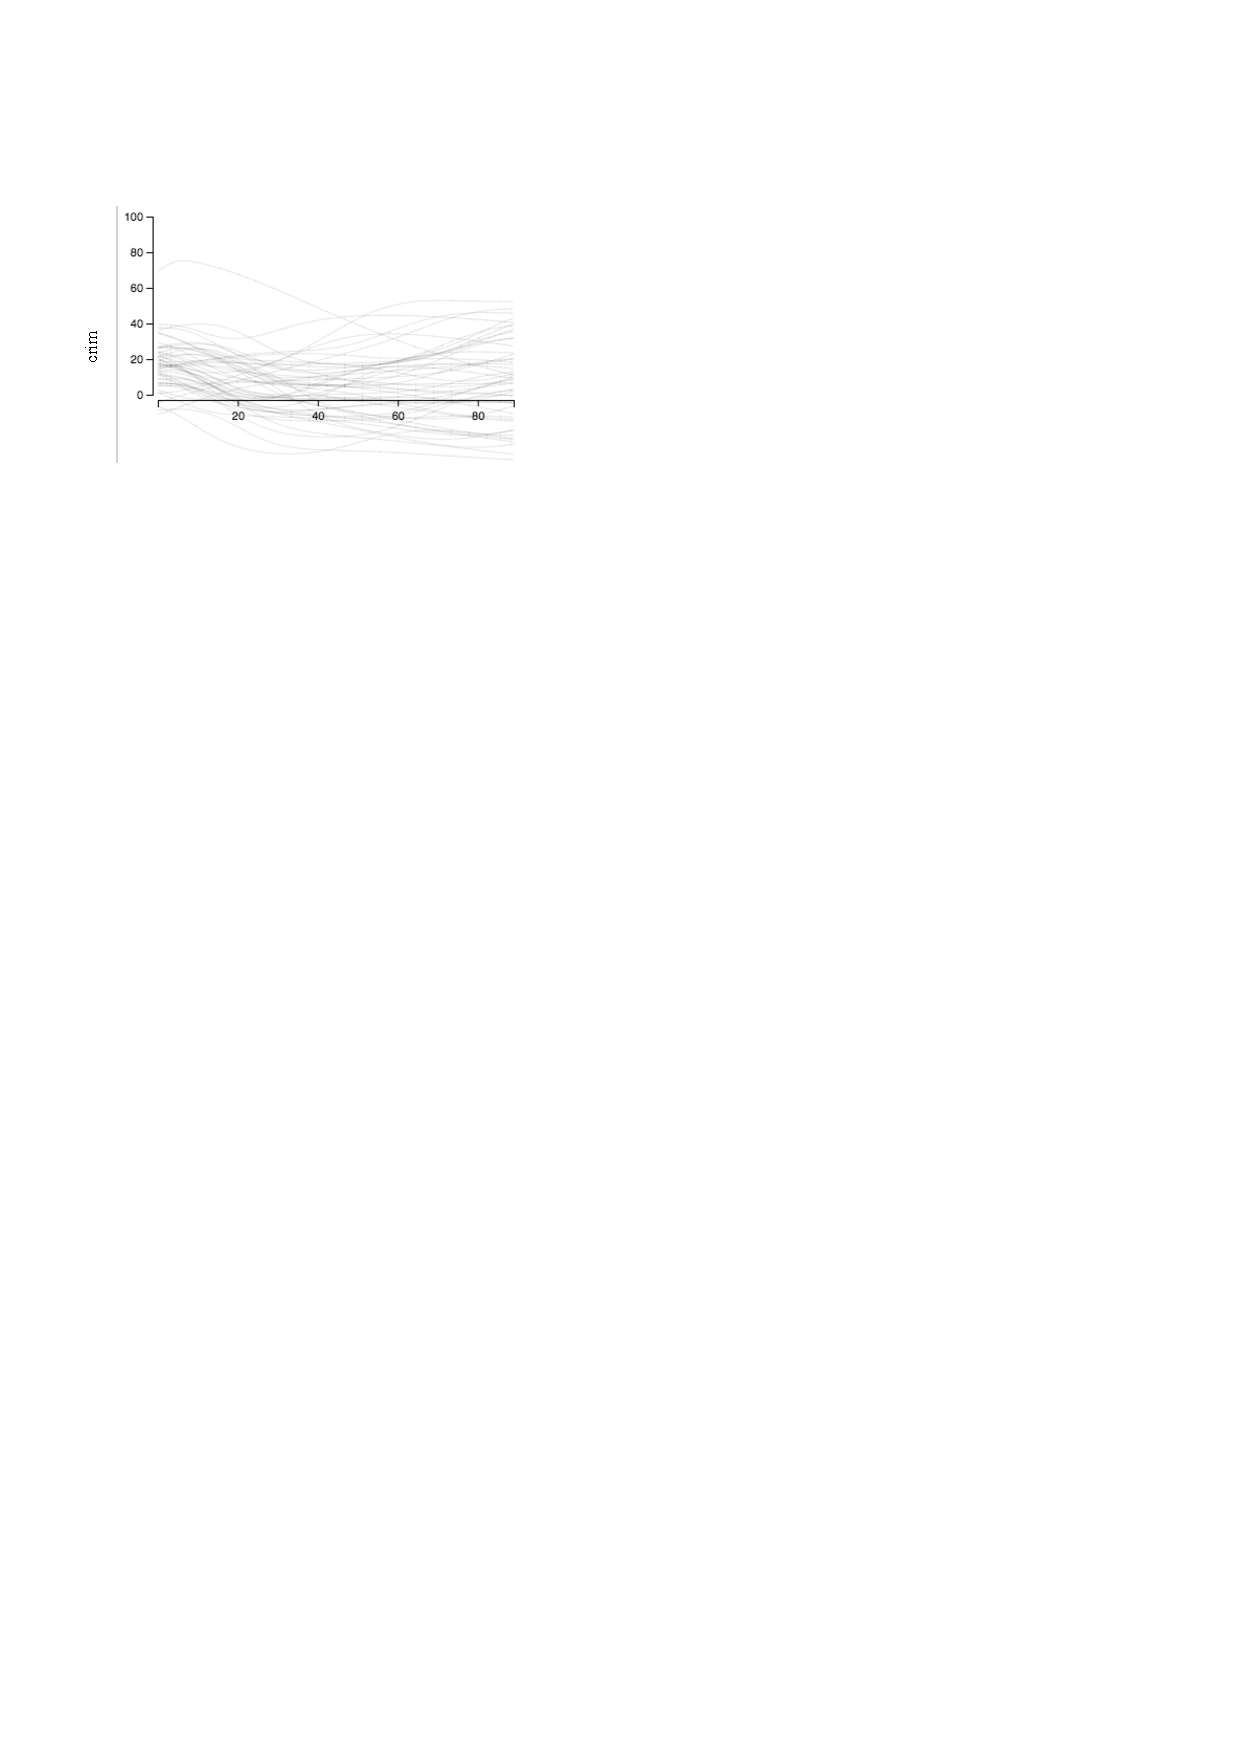
\includegraphics[width=0.1\textwidth]{nn26_1.pdf}
  &
    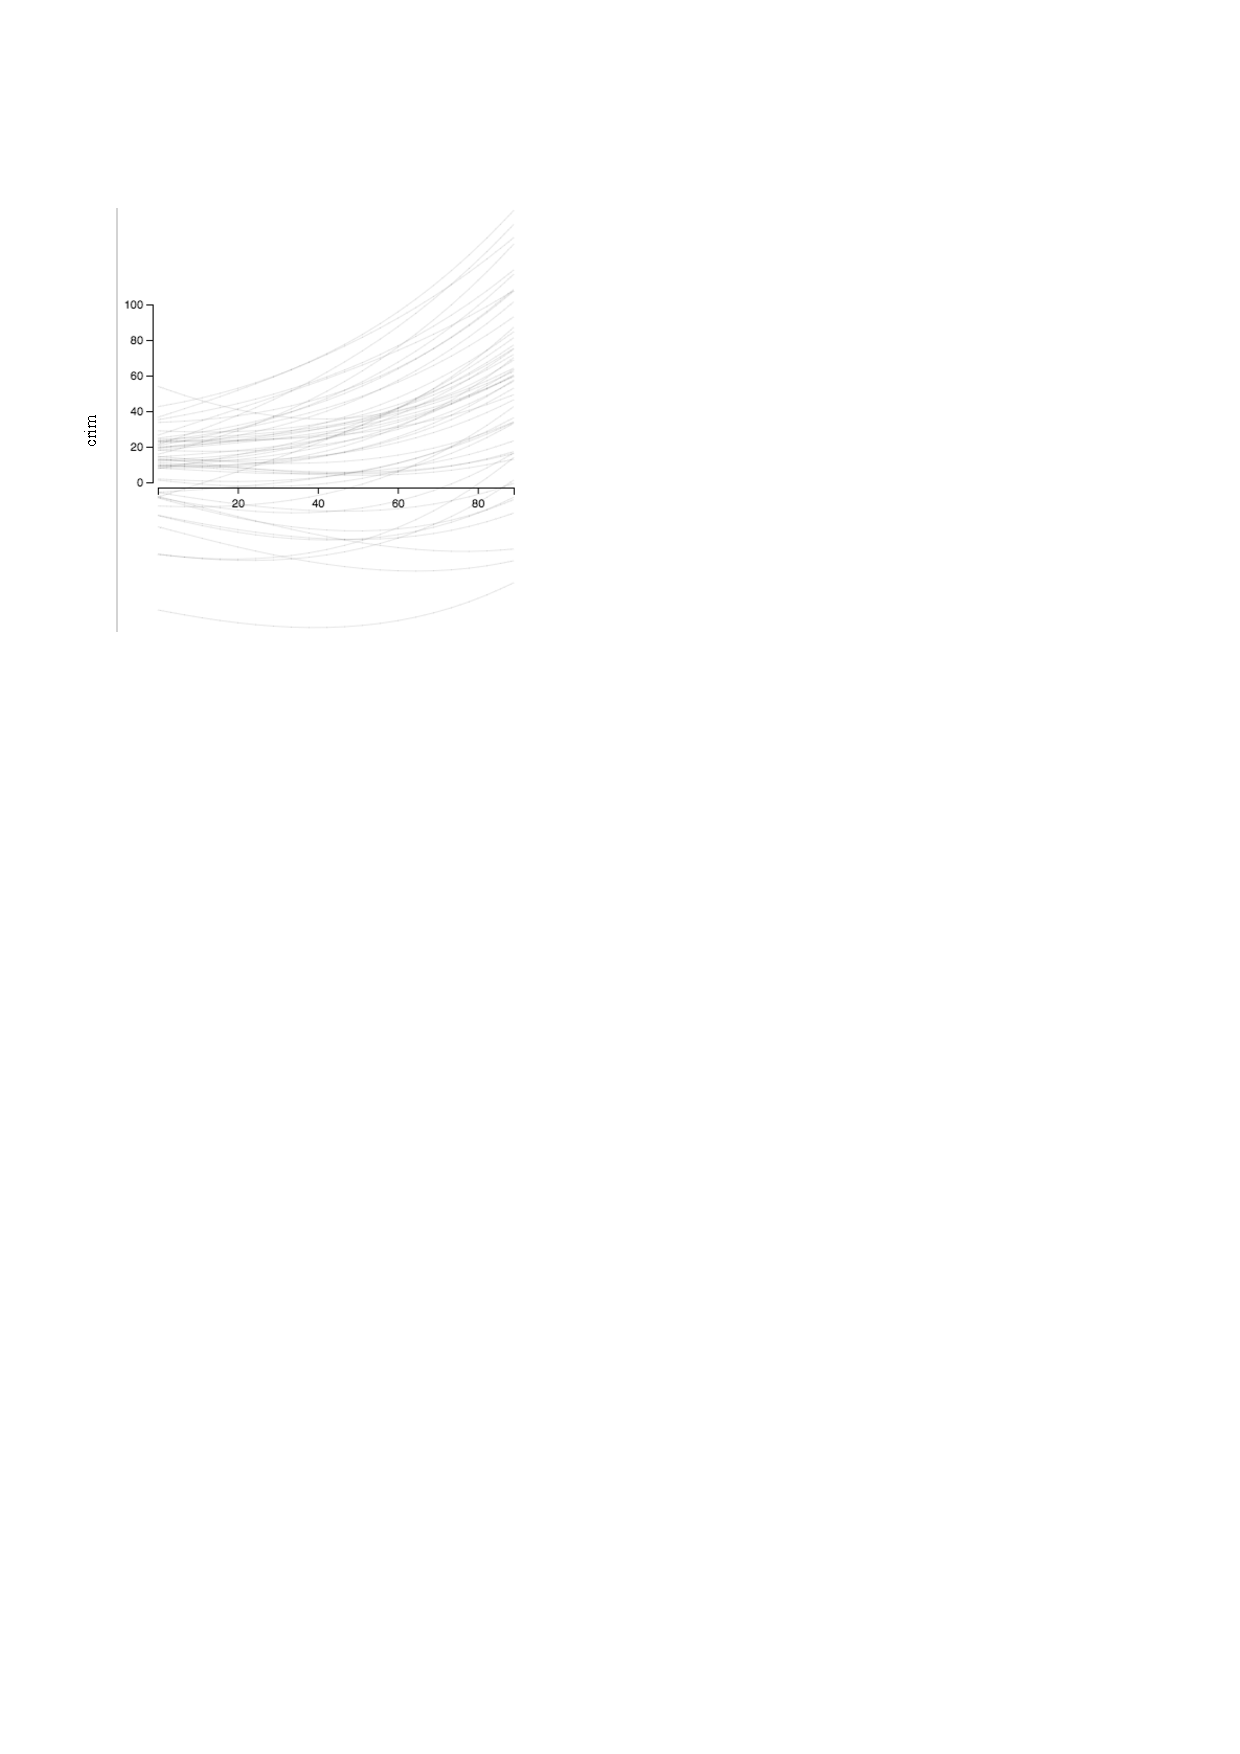
\includegraphics[width=0.1\textwidth]{svmp_1.pdf}
  &
    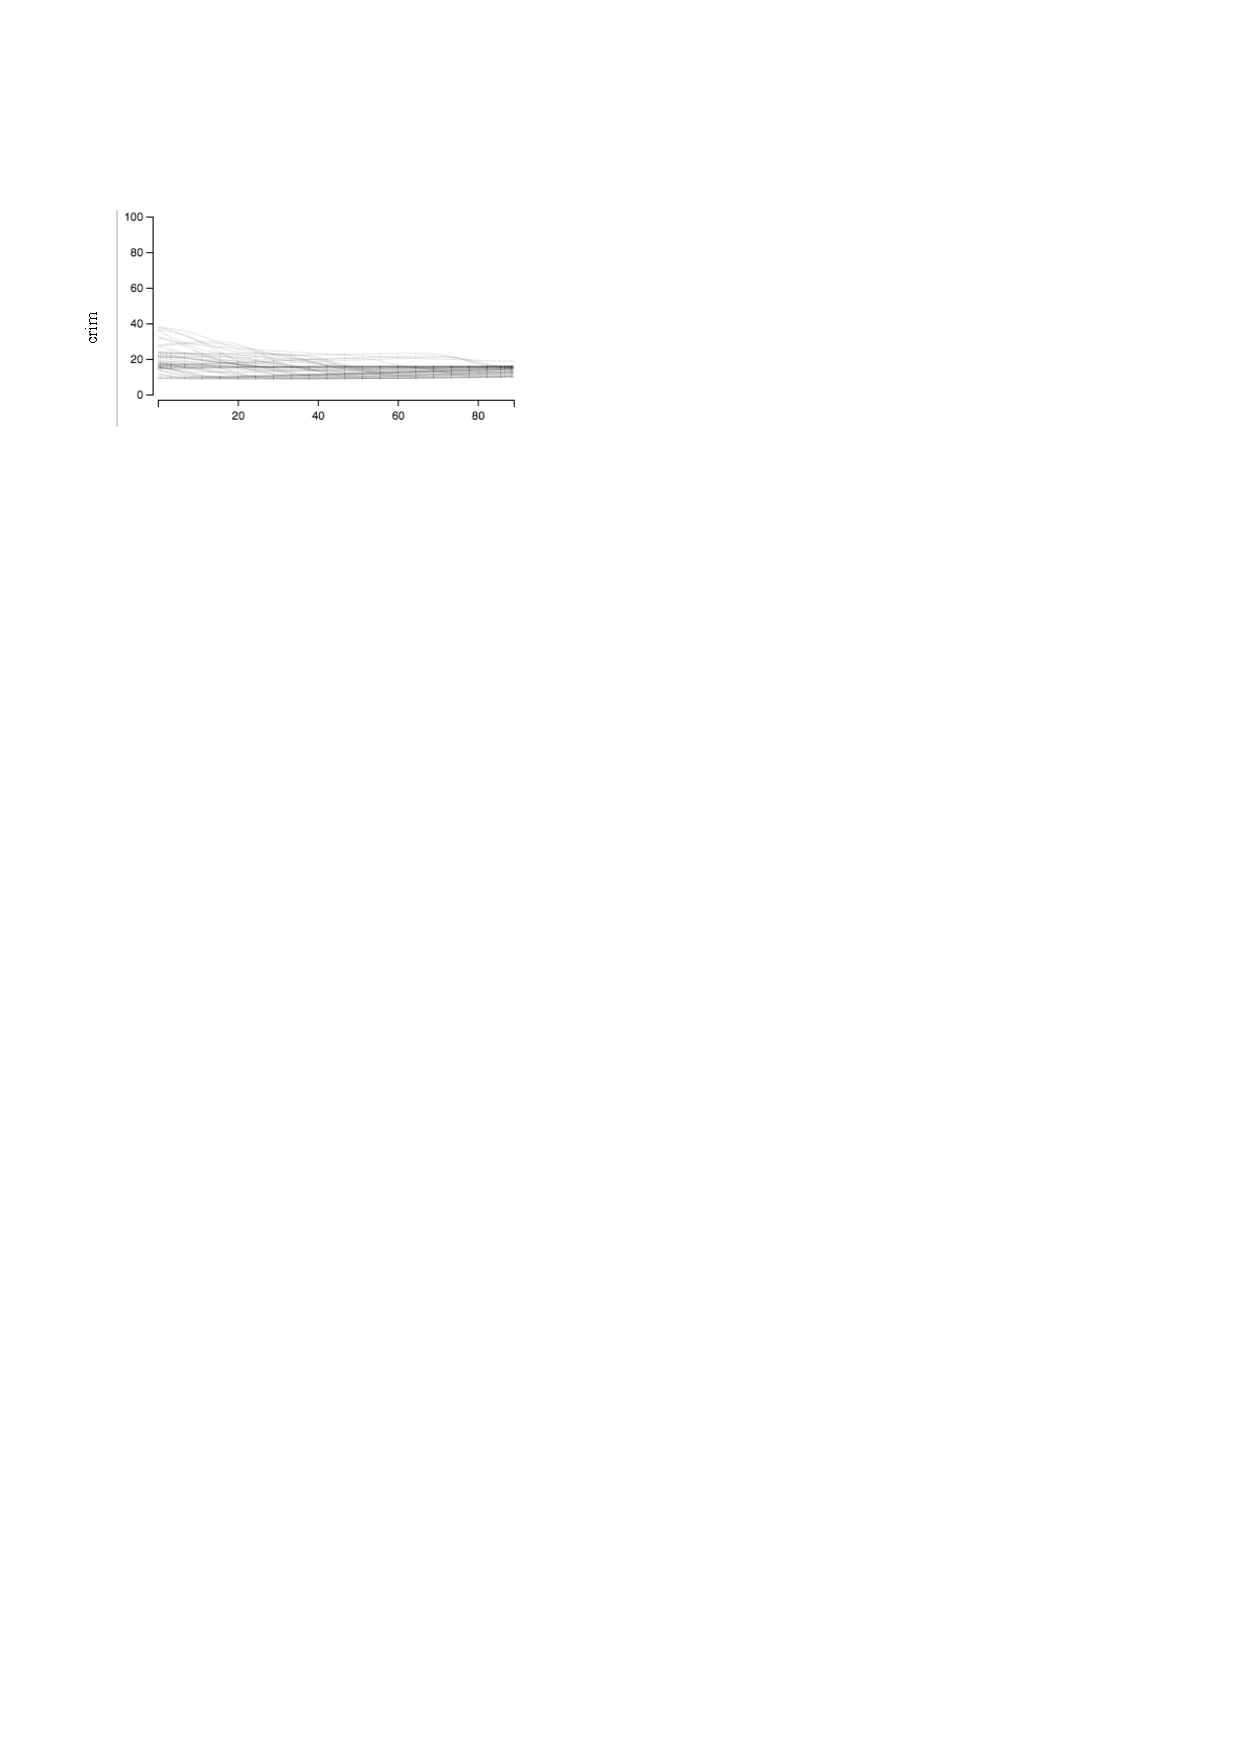
\includegraphics[width=0.1\textwidth]{nn5x3_1.pdf}
  &
    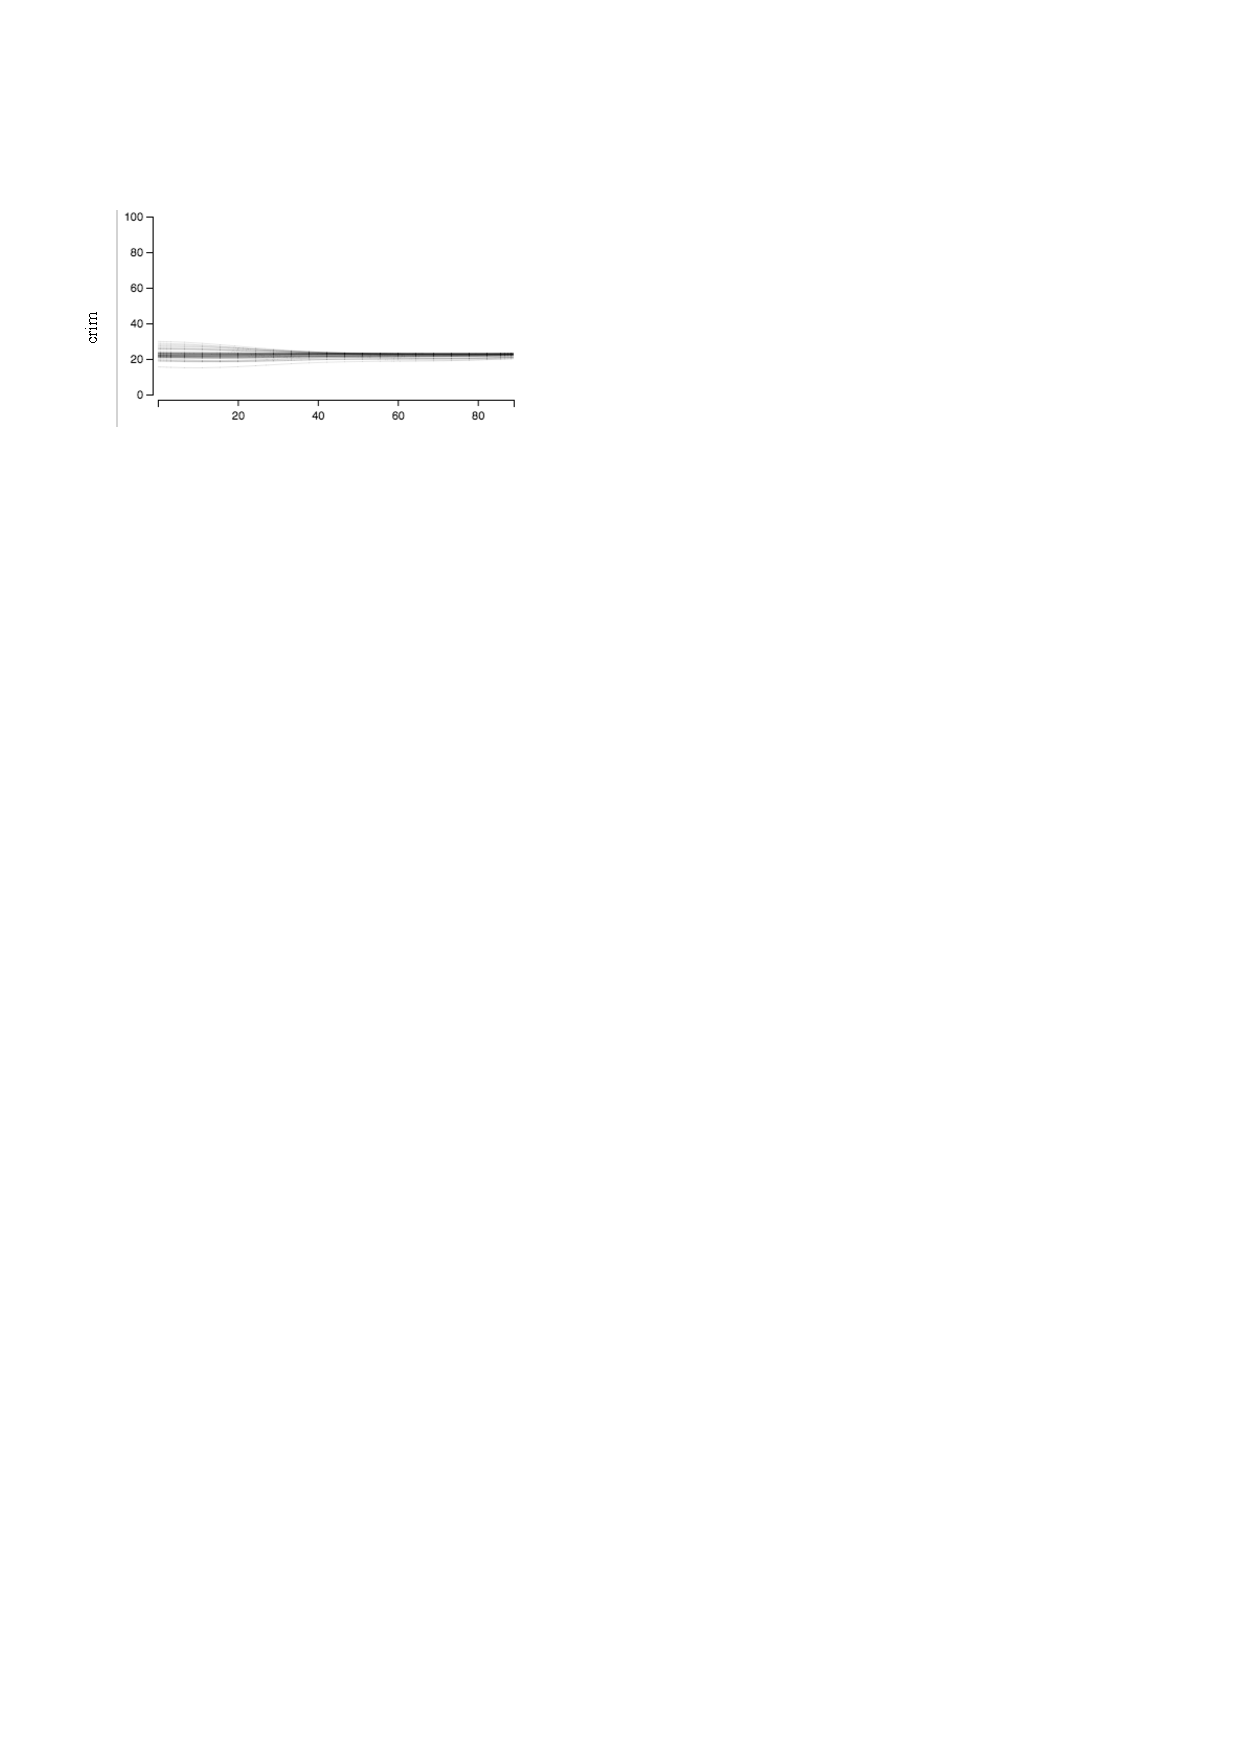
\includegraphics[width=0.1\textwidth]{svmr_1.pdf}
  \\
  \hline \\
  Residential lots over 25,000 sq.ft. &
    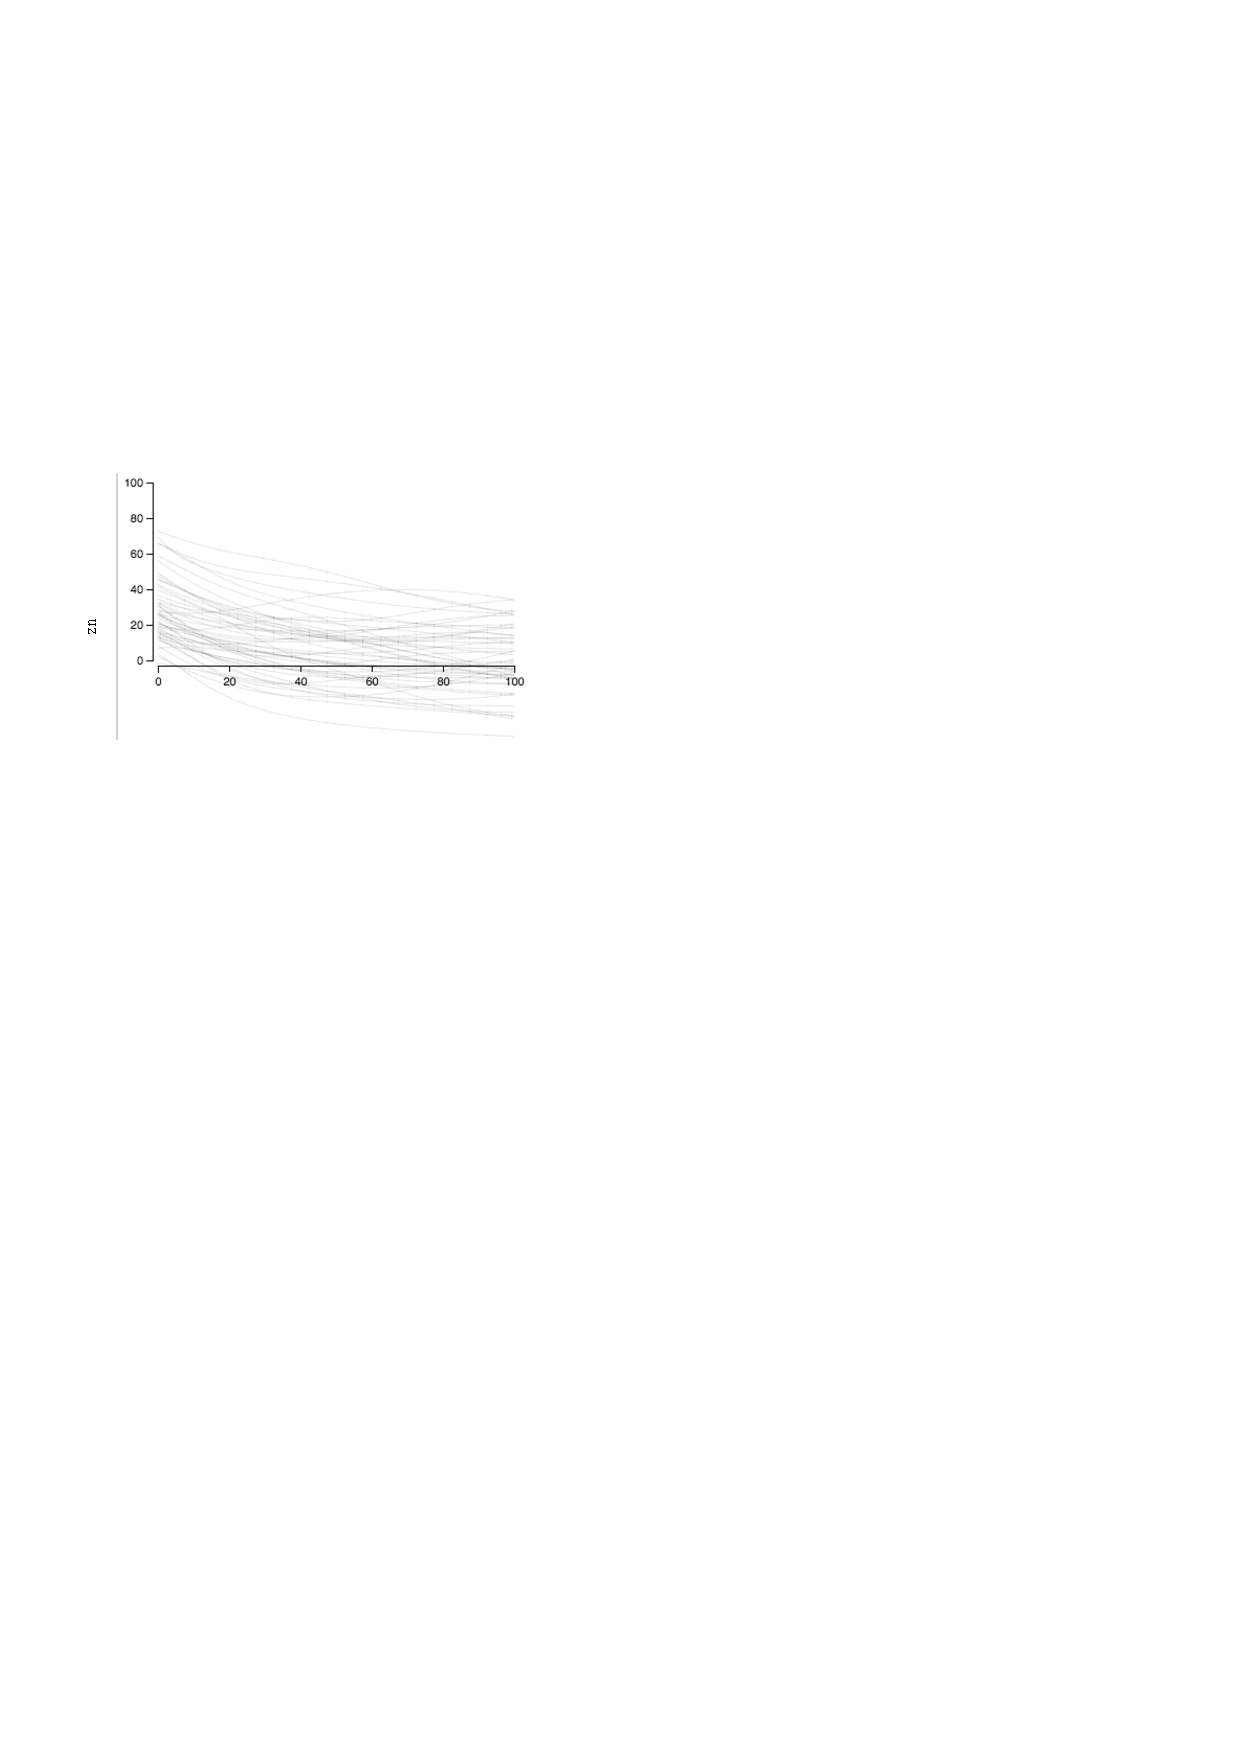
\includegraphics[width=0.1\textwidth]{nn26_2.pdf}
  &
    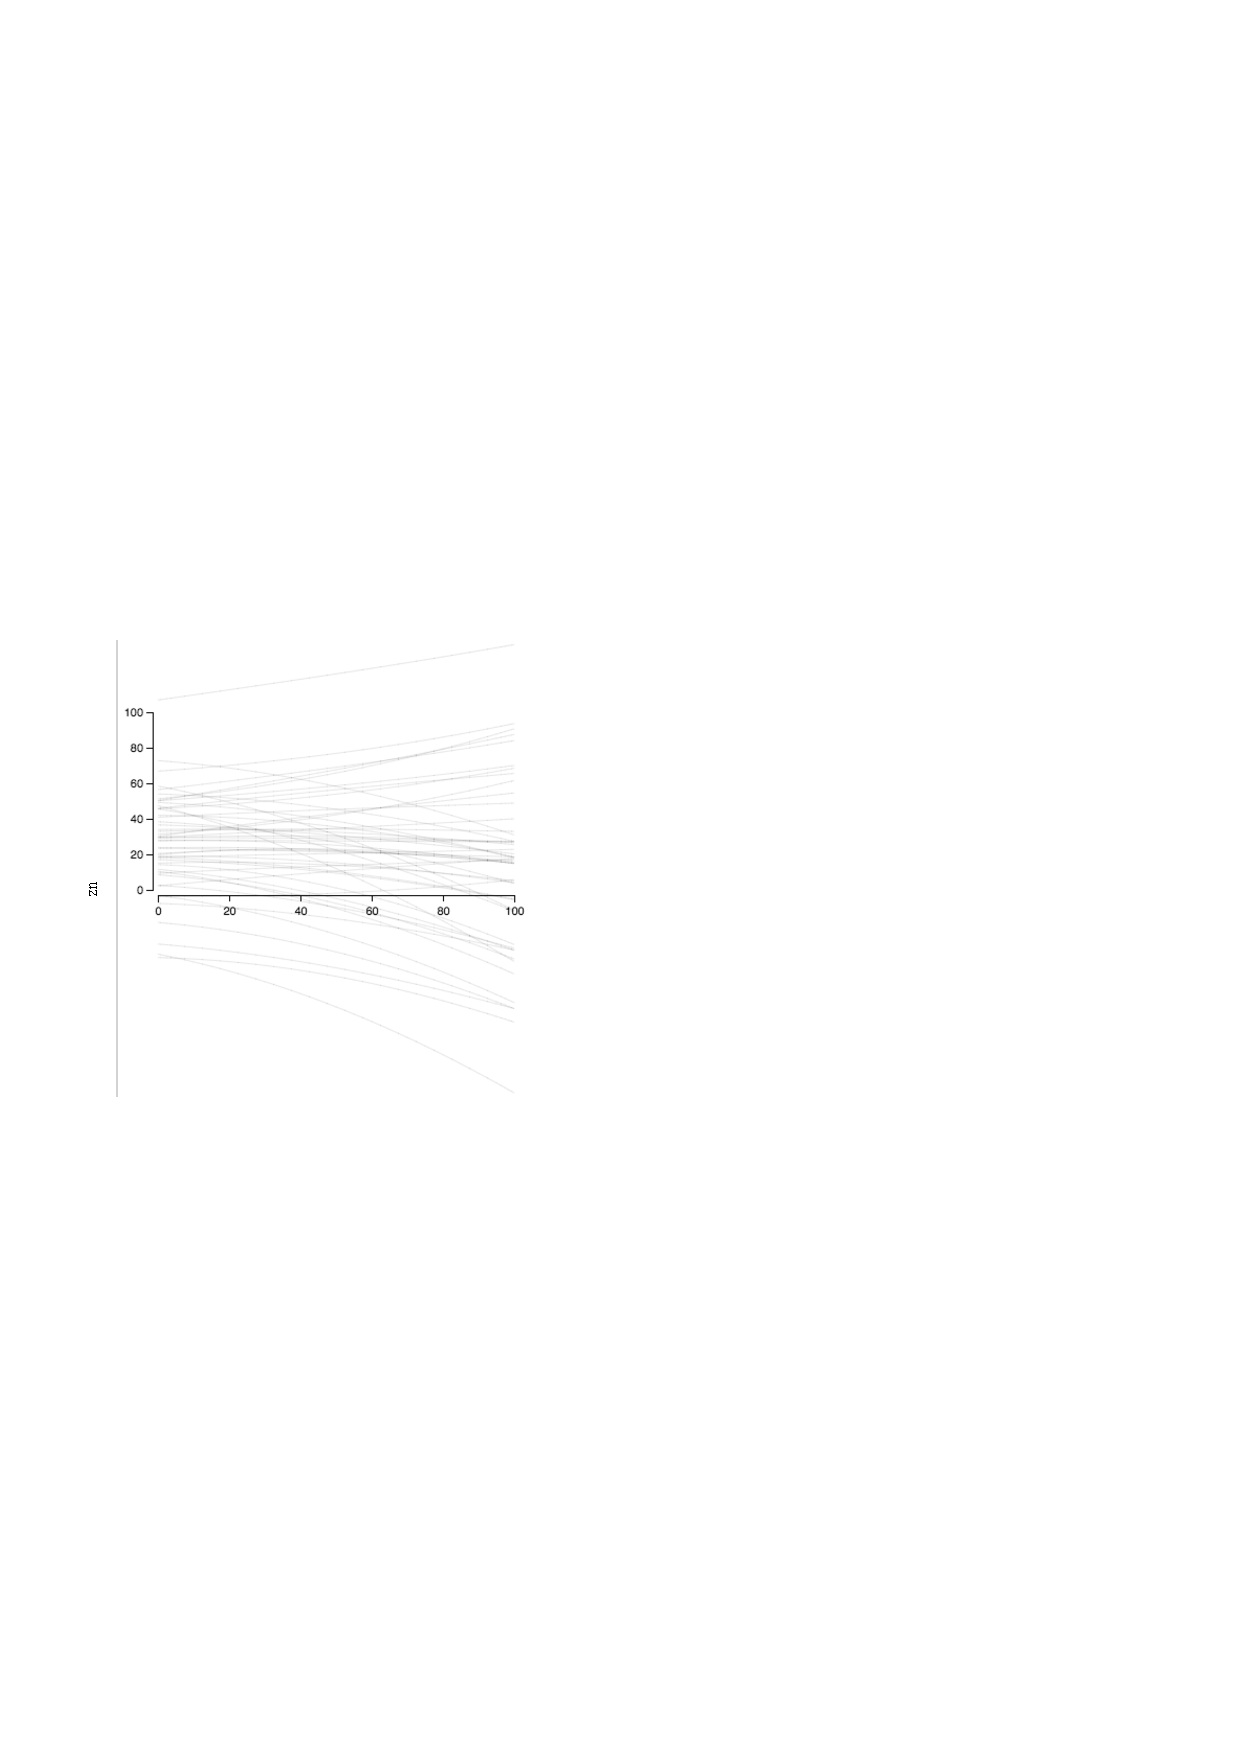
\includegraphics[width=0.1\textwidth]{svmp_2.pdf}
  &
    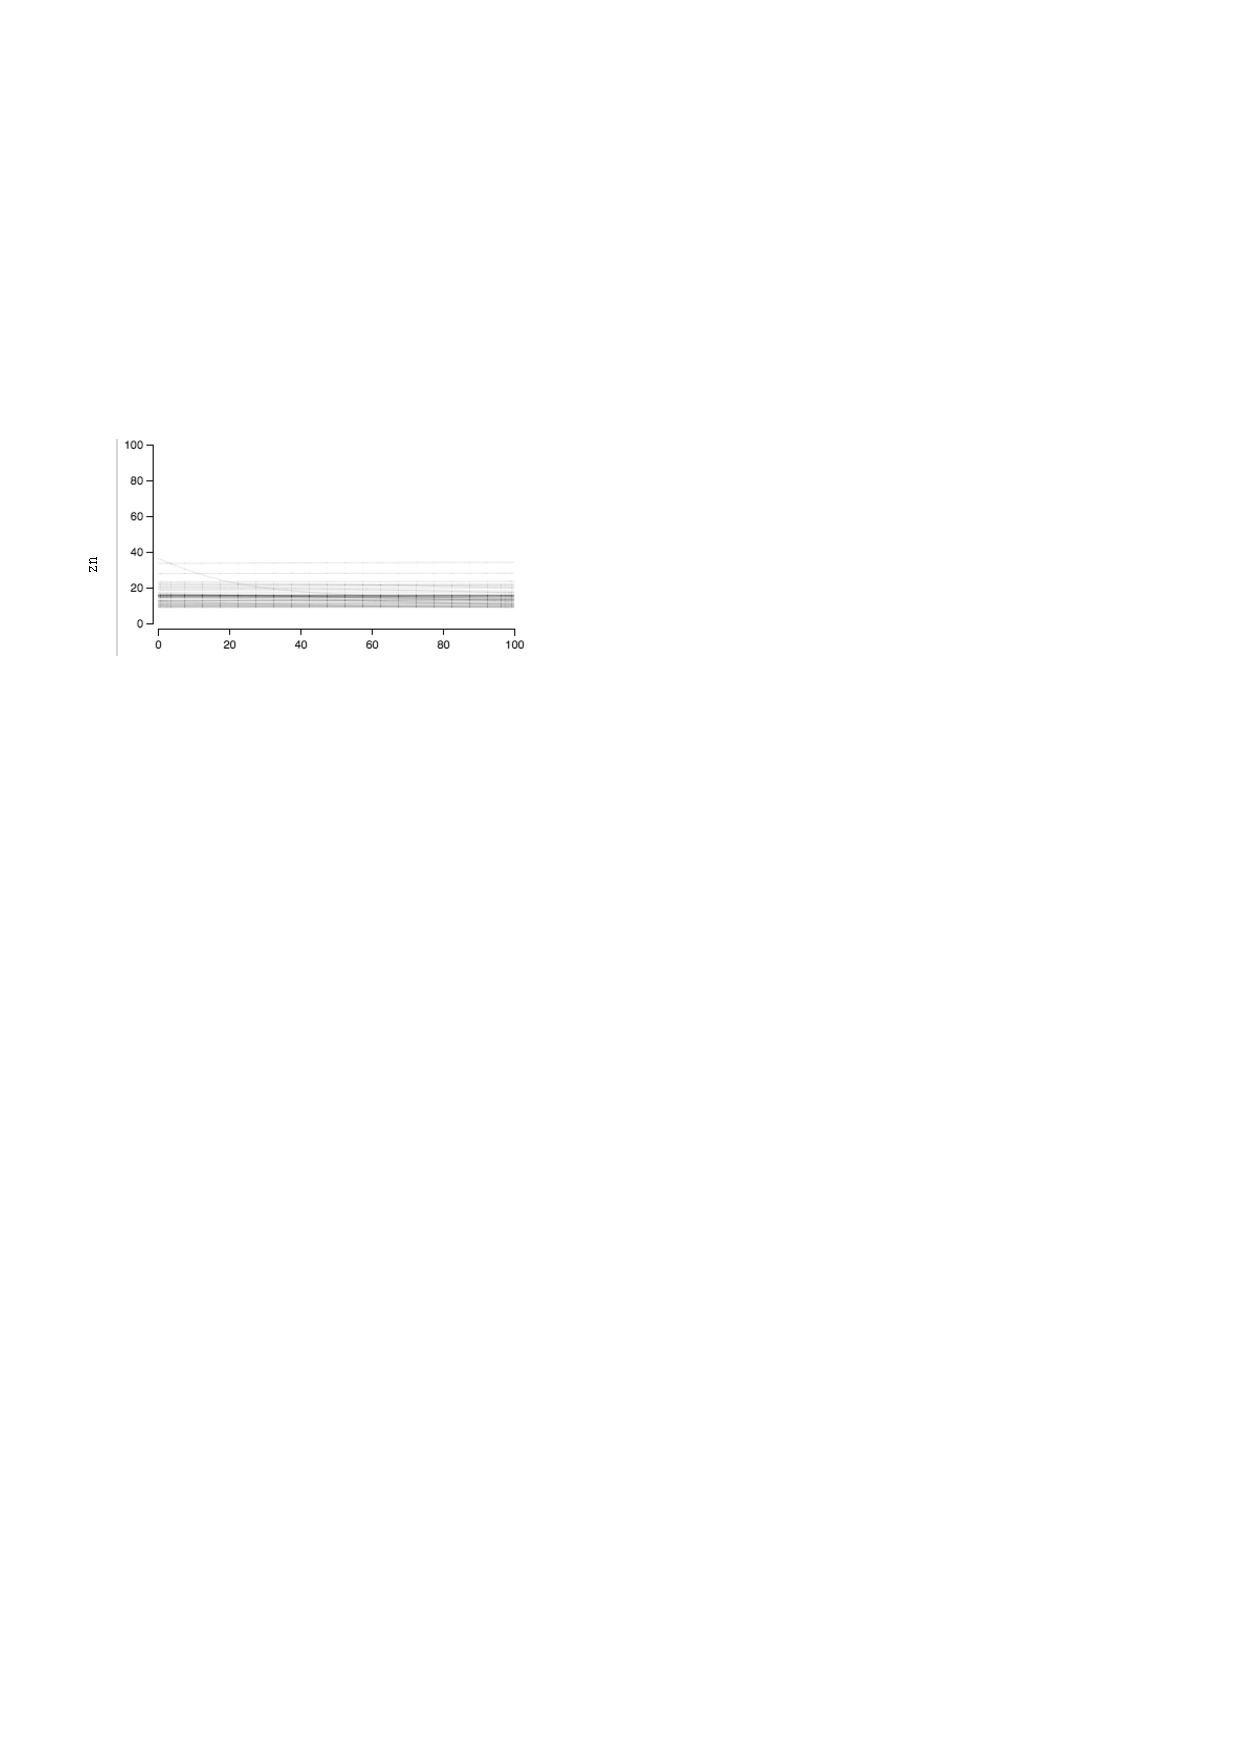
\includegraphics[width=0.1\textwidth]{nn5x3_2.pdf}
  &
    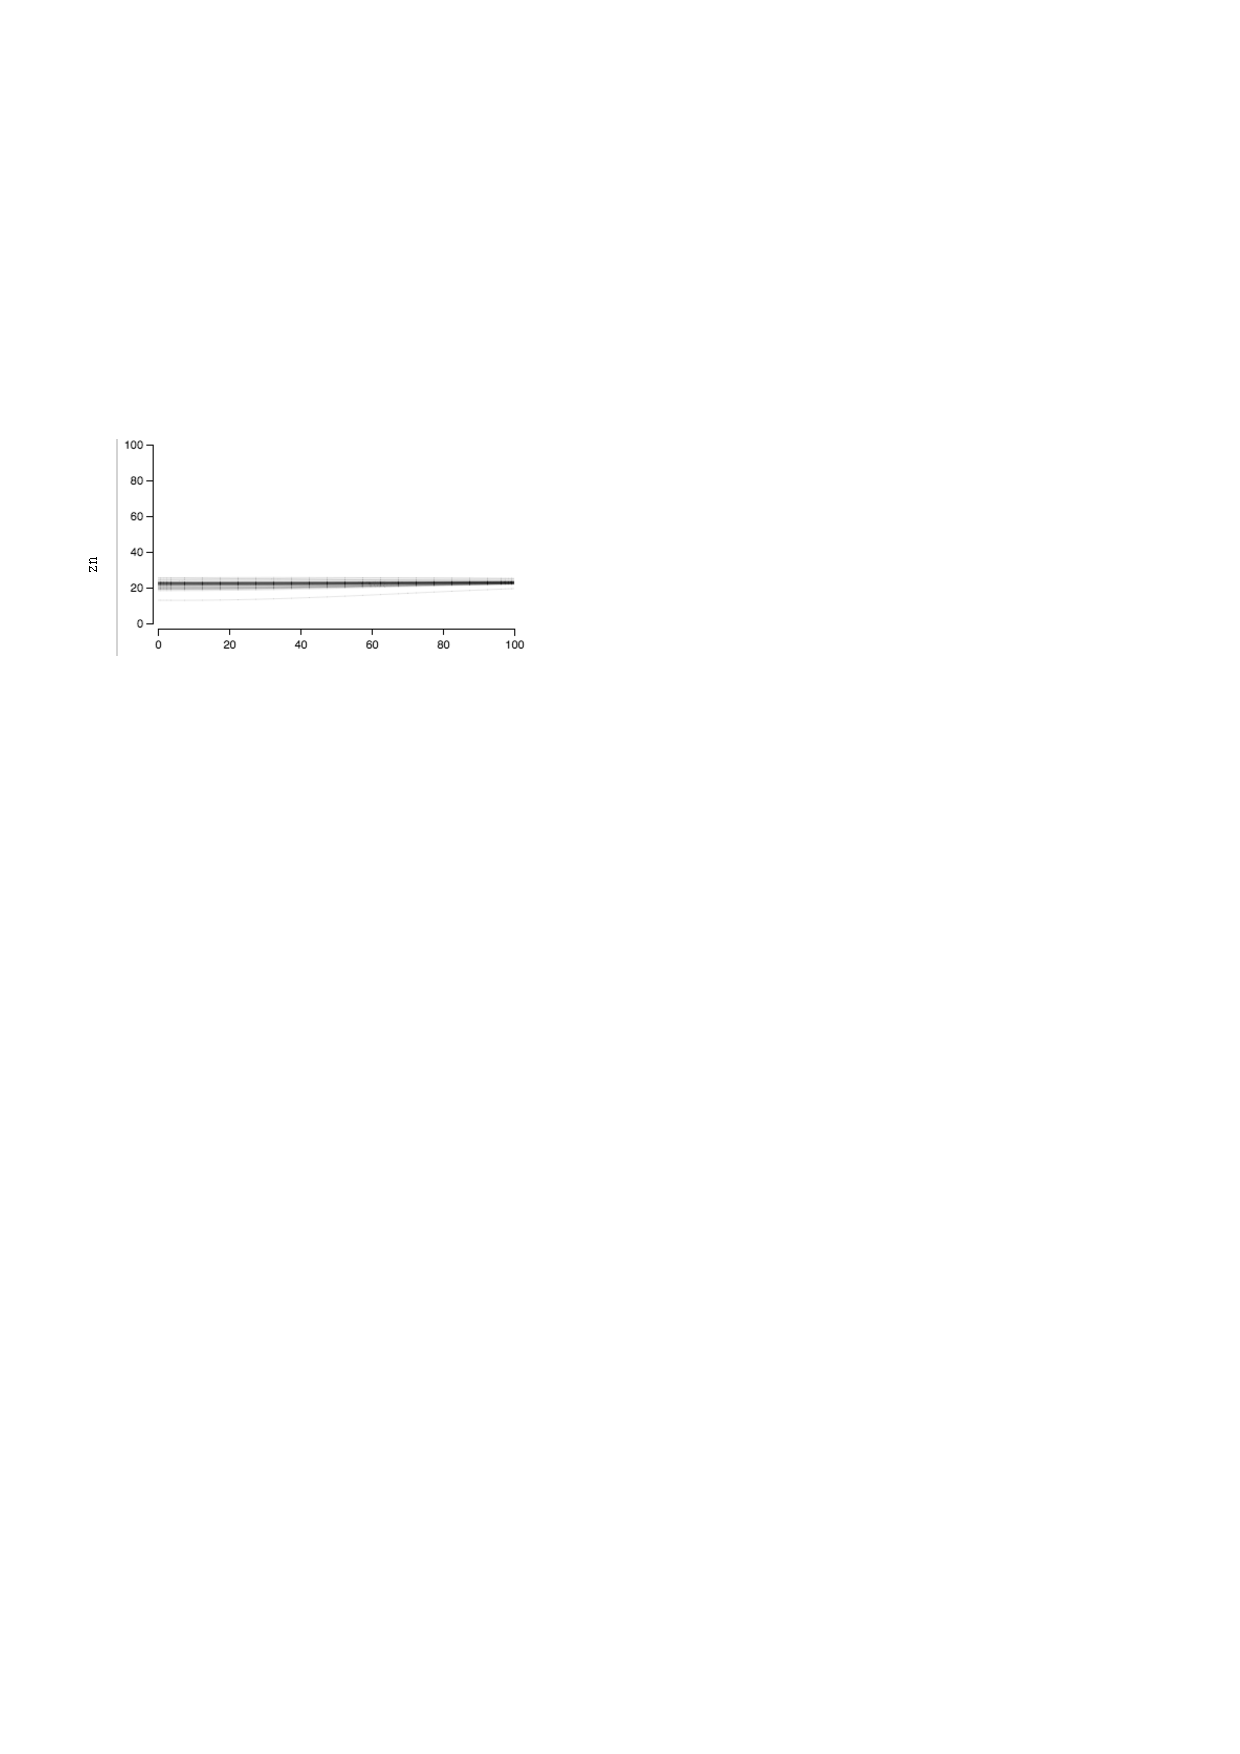
\includegraphics[width=0.1\textwidth]{svmr_2.pdf}
  \\
  \hline \\
  Non-retail business acres &
    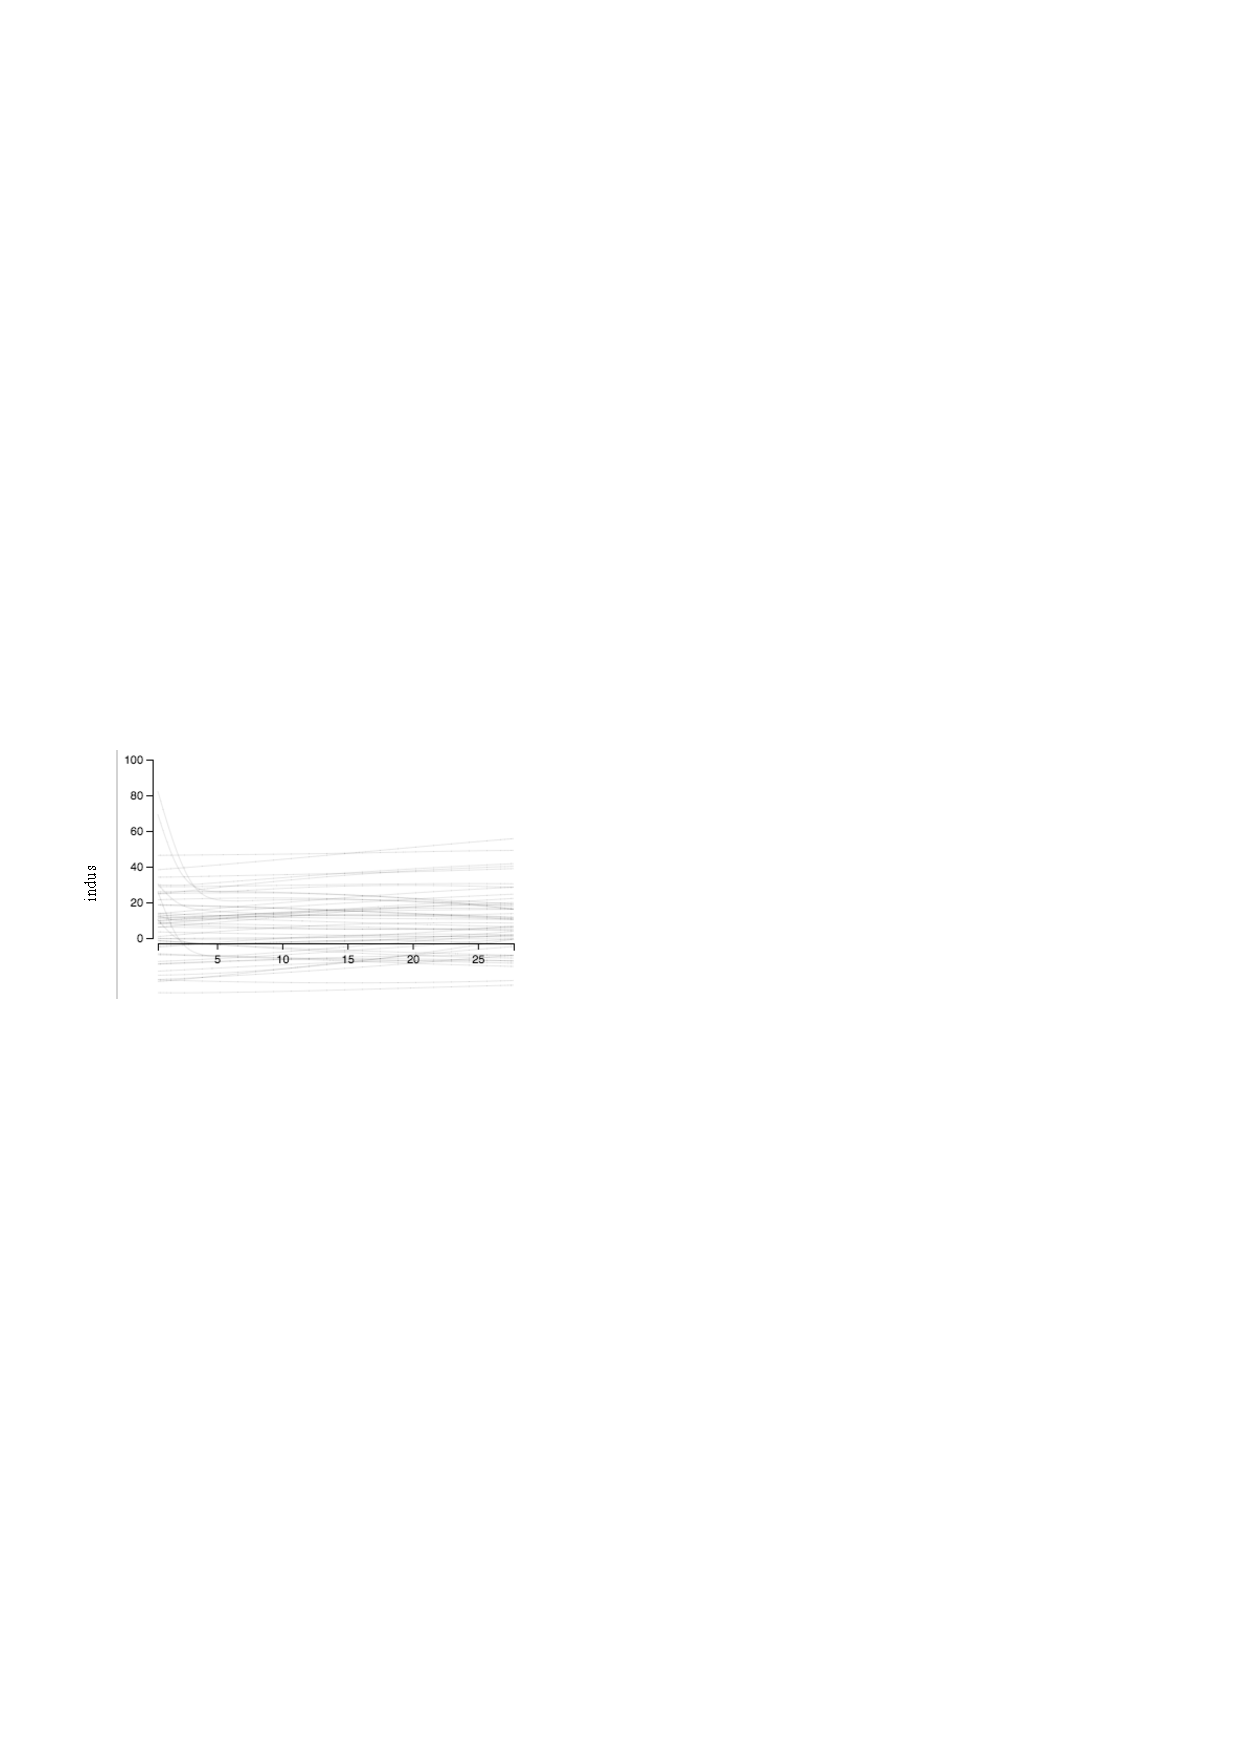
\includegraphics[width=0.1\textwidth]{nn26_3.pdf}
  &
    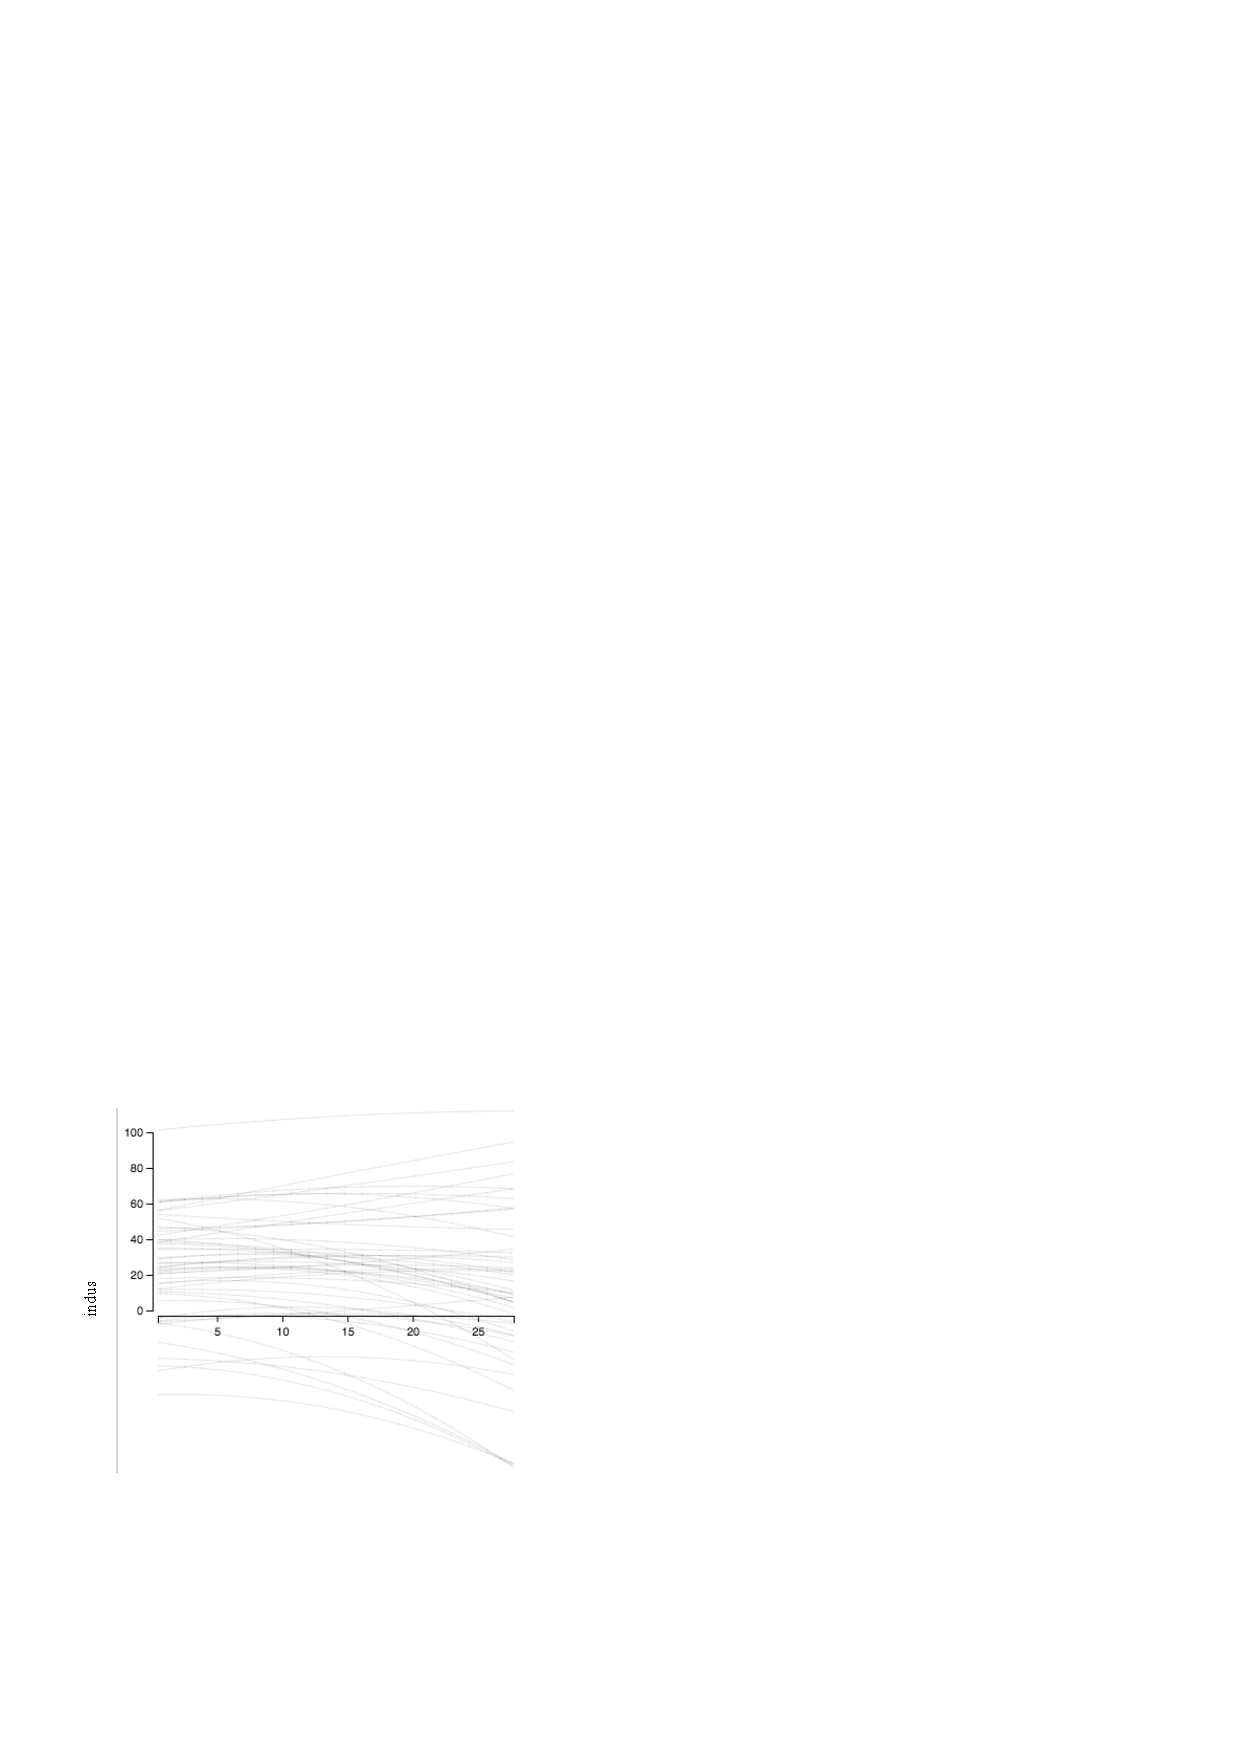
\includegraphics[width=0.1\textwidth]{svmp_3.pdf}
  &
    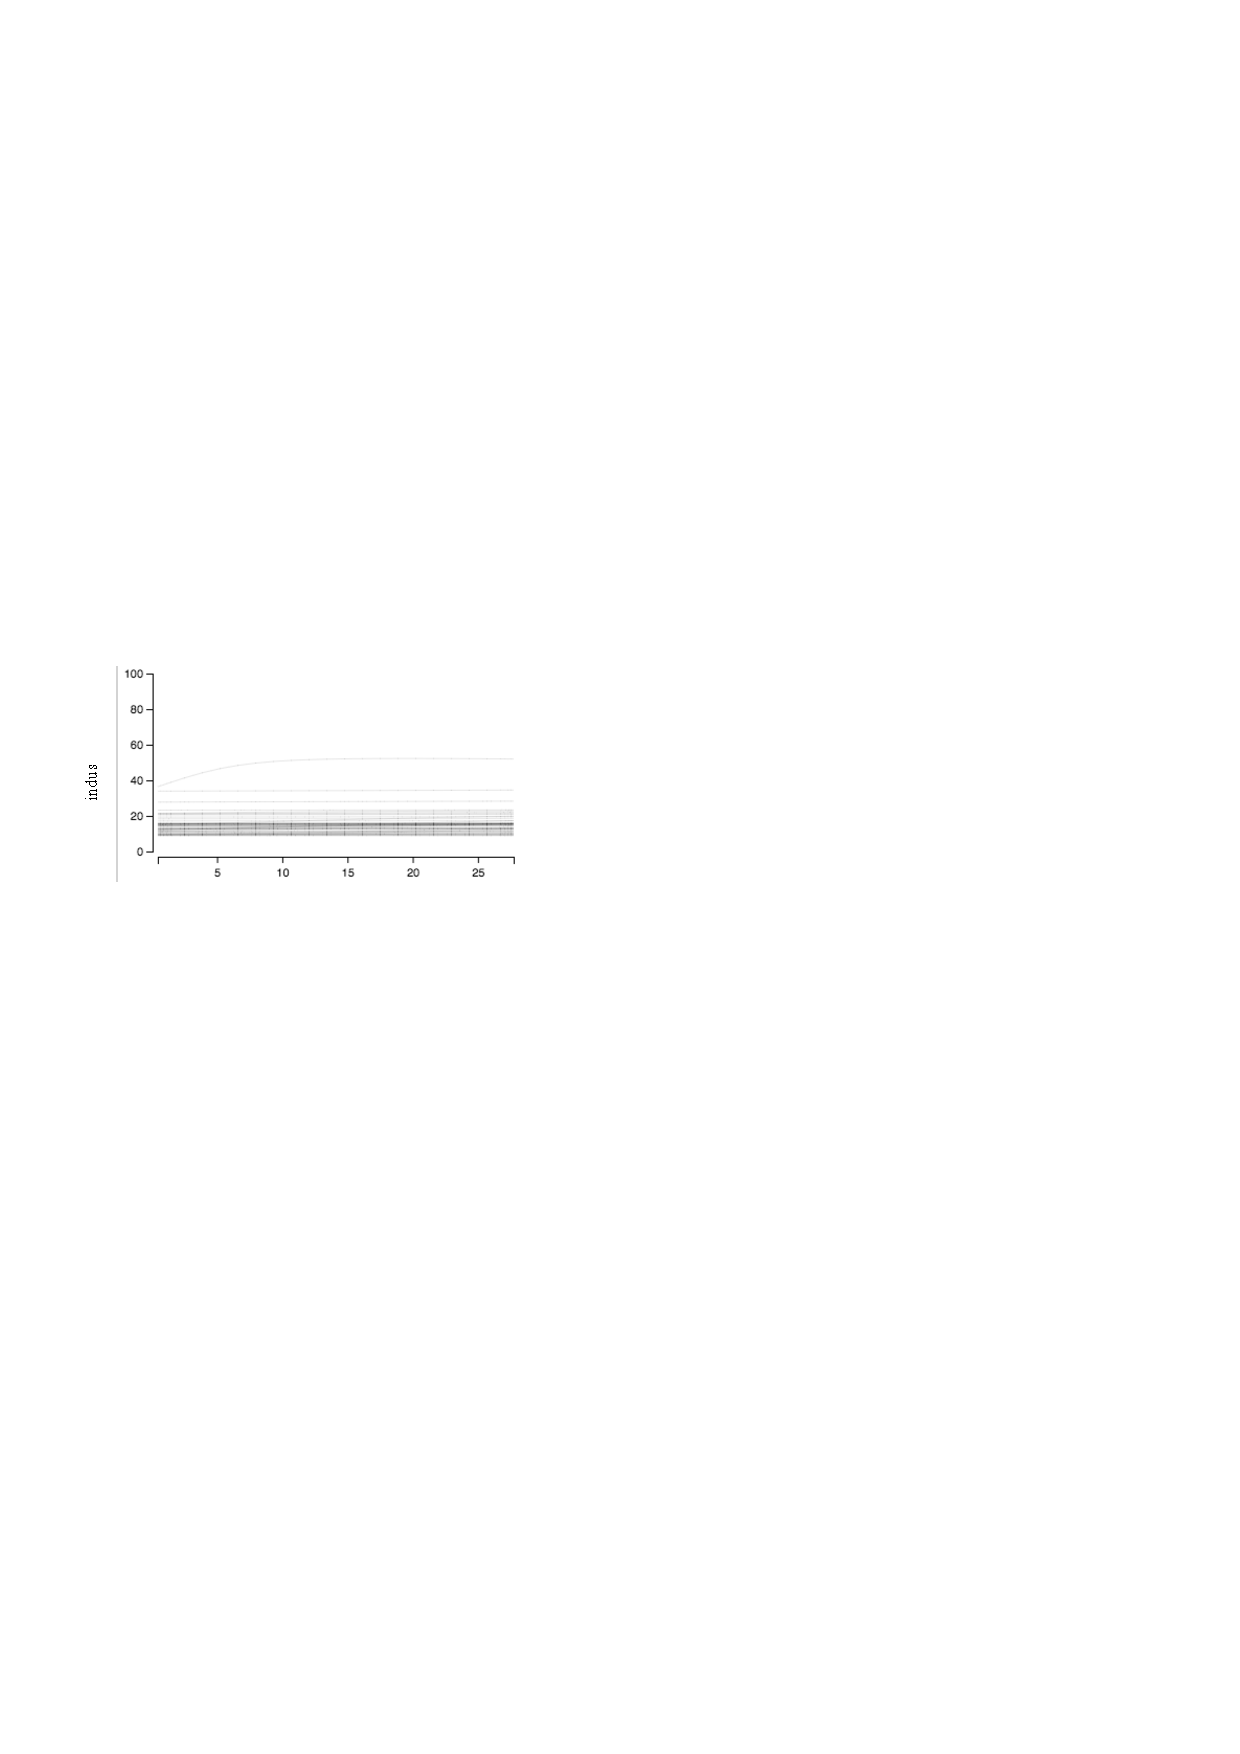
\includegraphics[width=0.1\textwidth]{nn5x3_3.pdf}
  &
    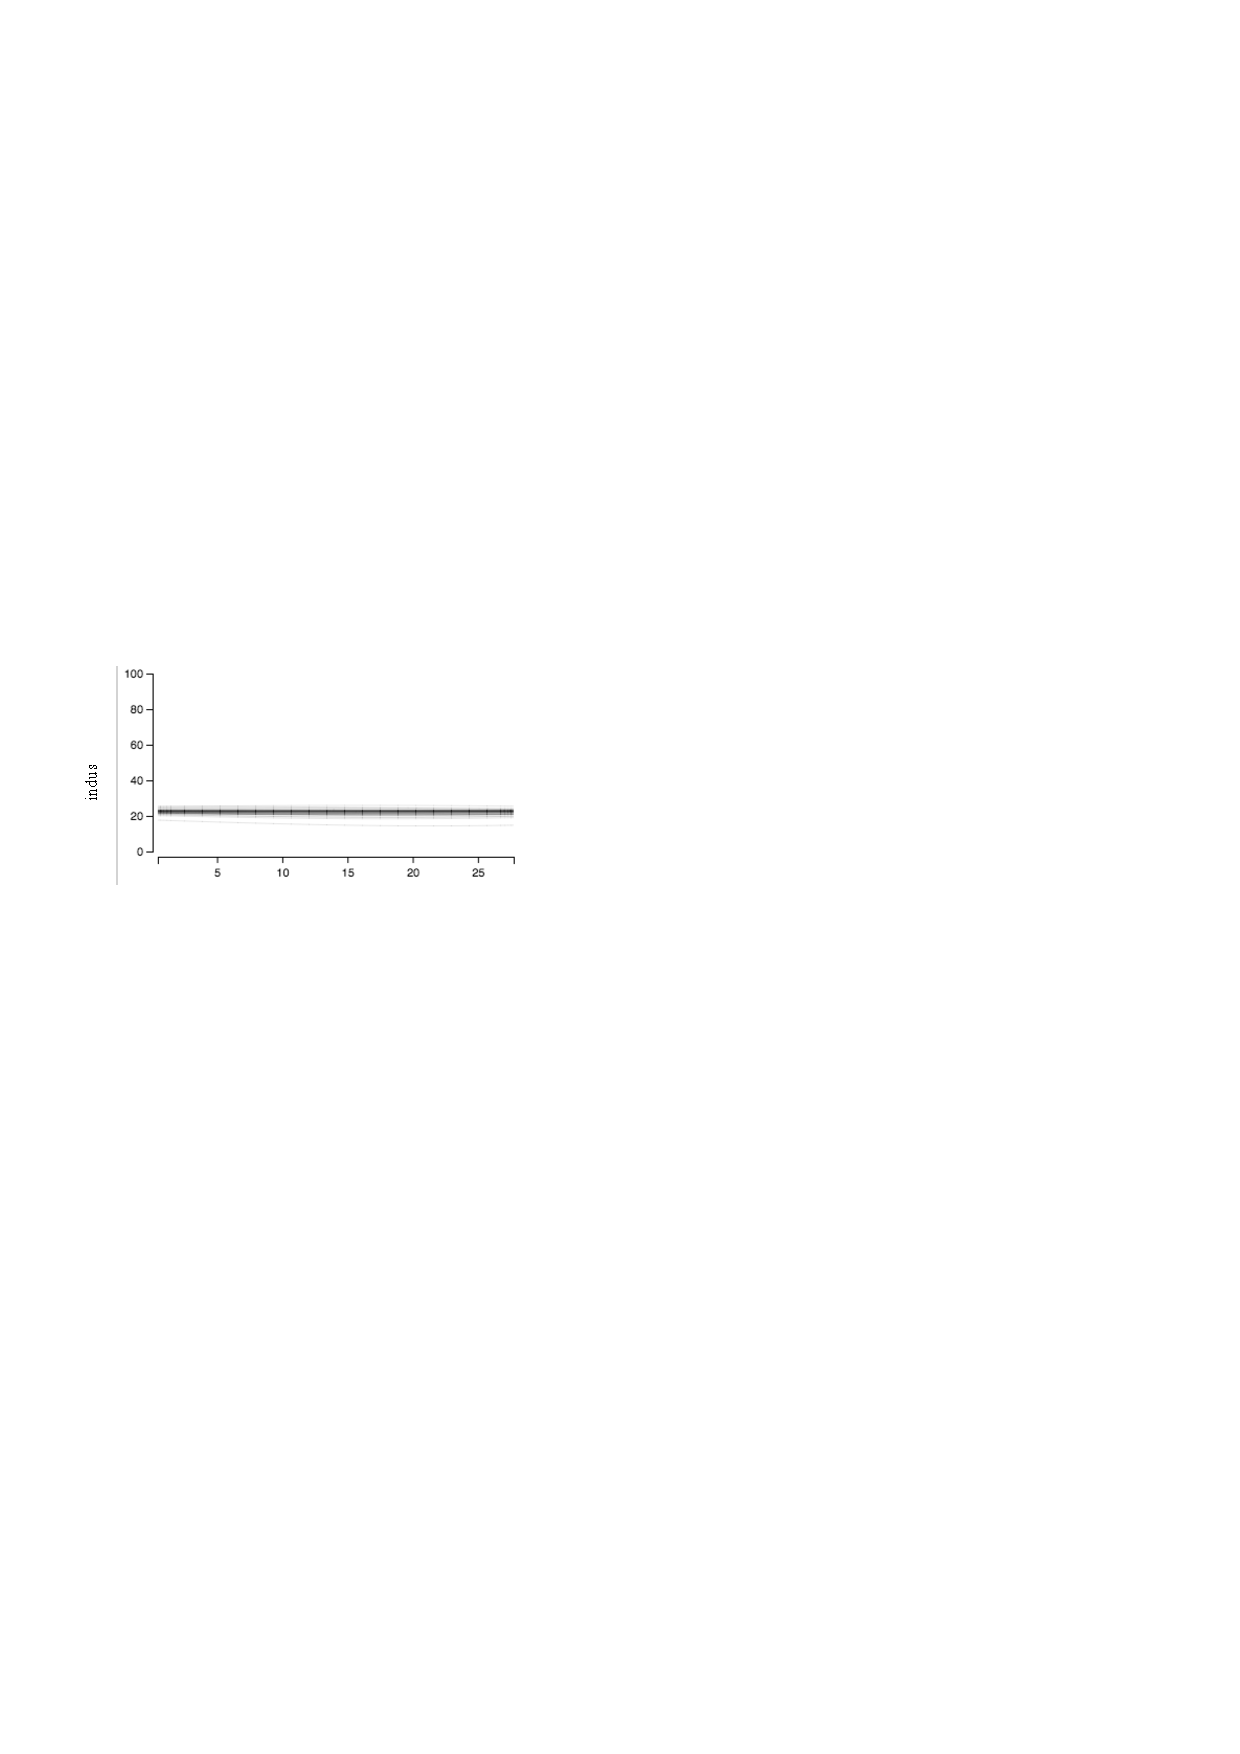
\includegraphics[width=0.1\textwidth]{svmr_3.pdf}
  \\
  \hline \\
  1 if tract bounds river &
    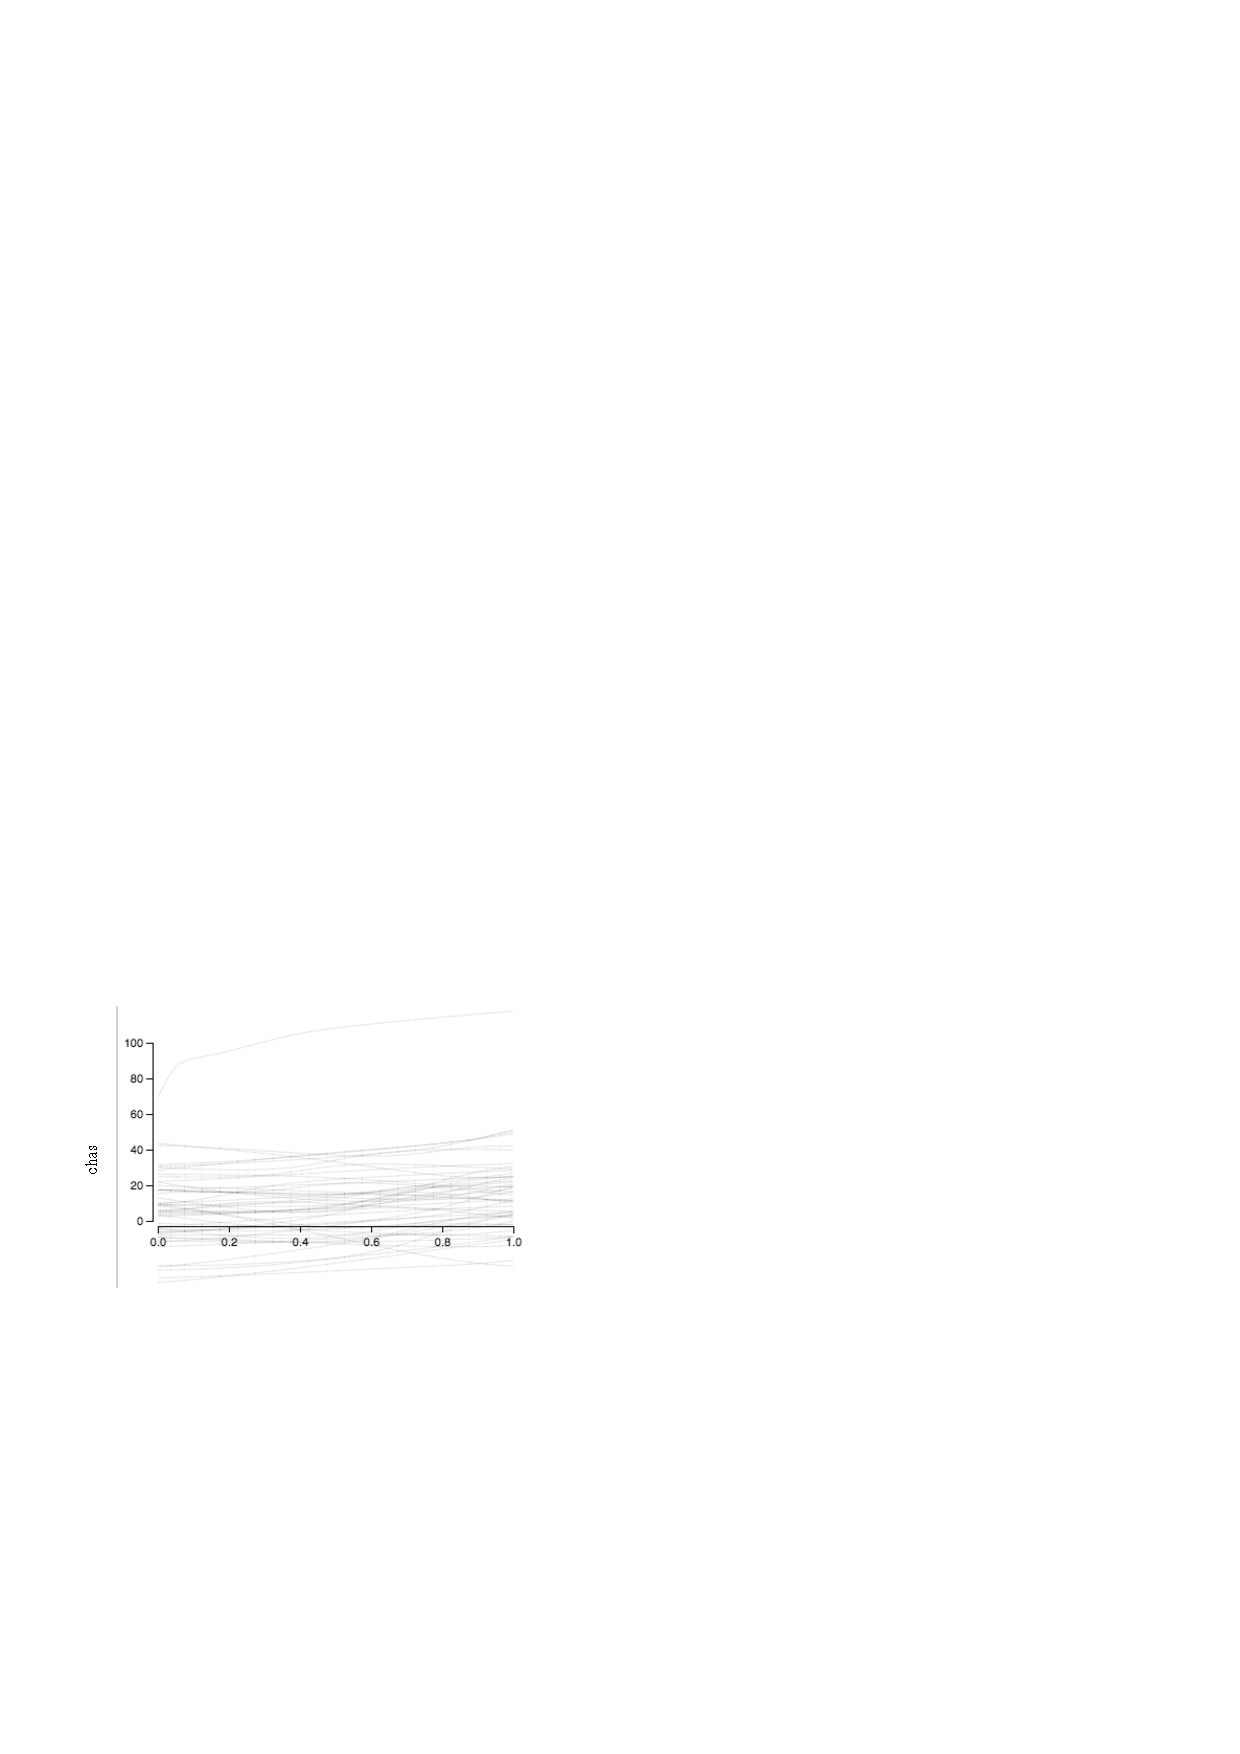
\includegraphics[width=0.1\textwidth]{nn26_4.pdf}
  &
    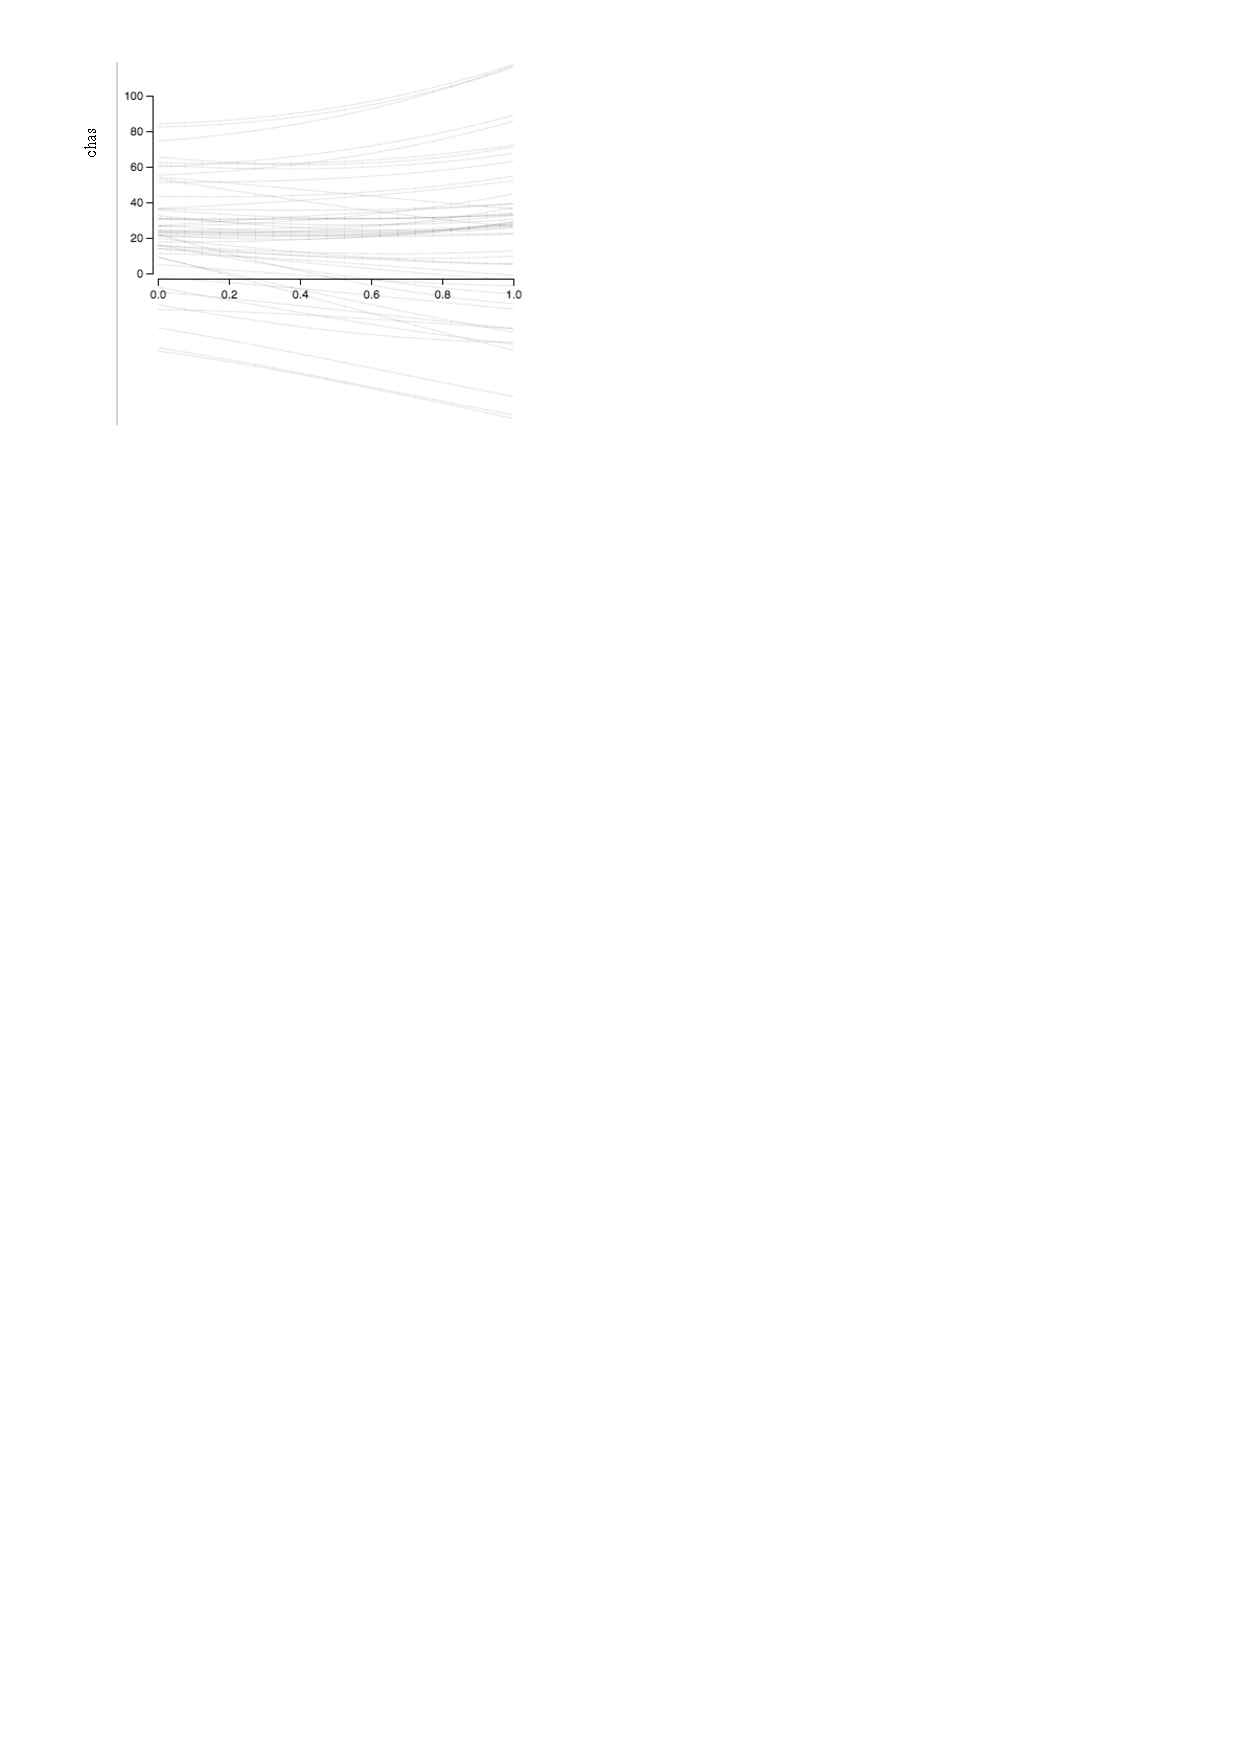
\includegraphics[width=0.1\textwidth]{svmp_4.pdf}
  &
    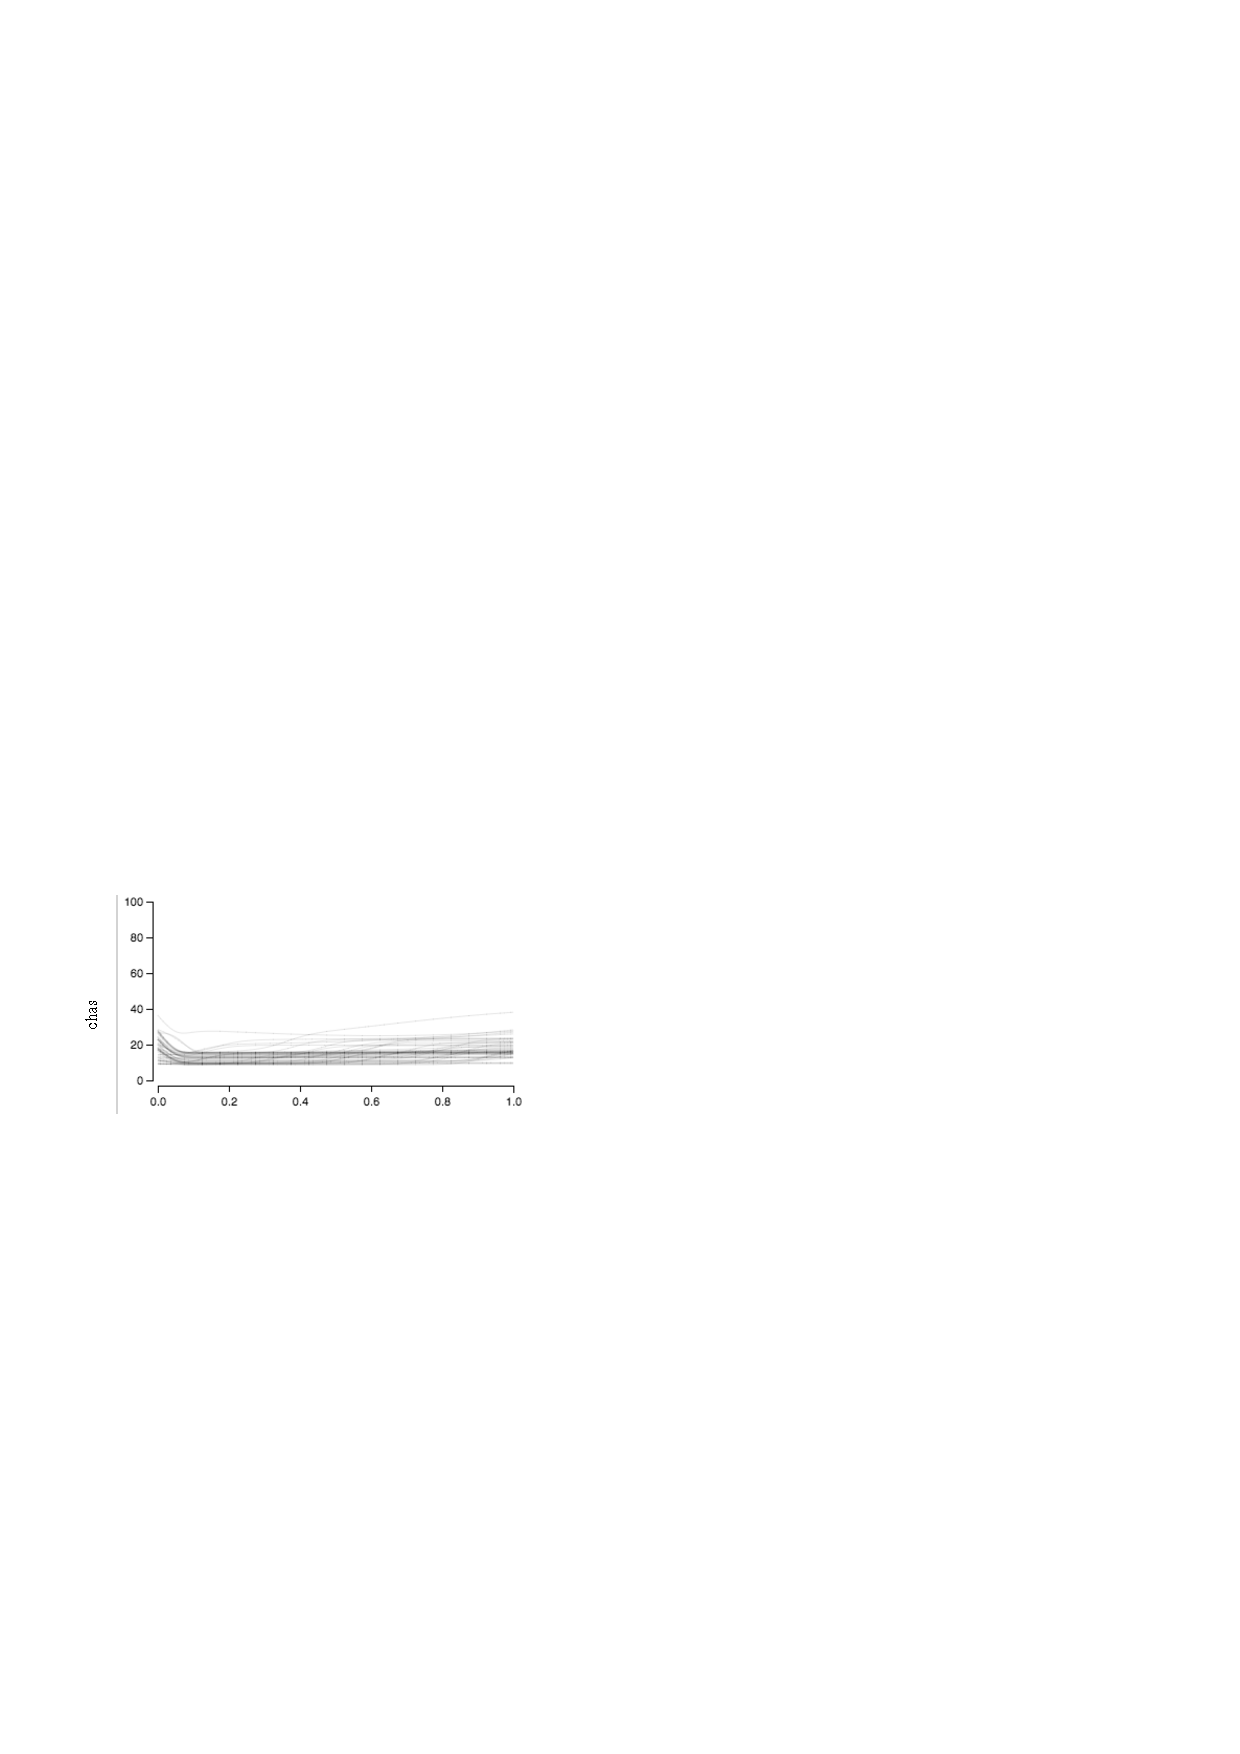
\includegraphics[width=0.1\textwidth]{nn5x3_4.pdf}
  &
    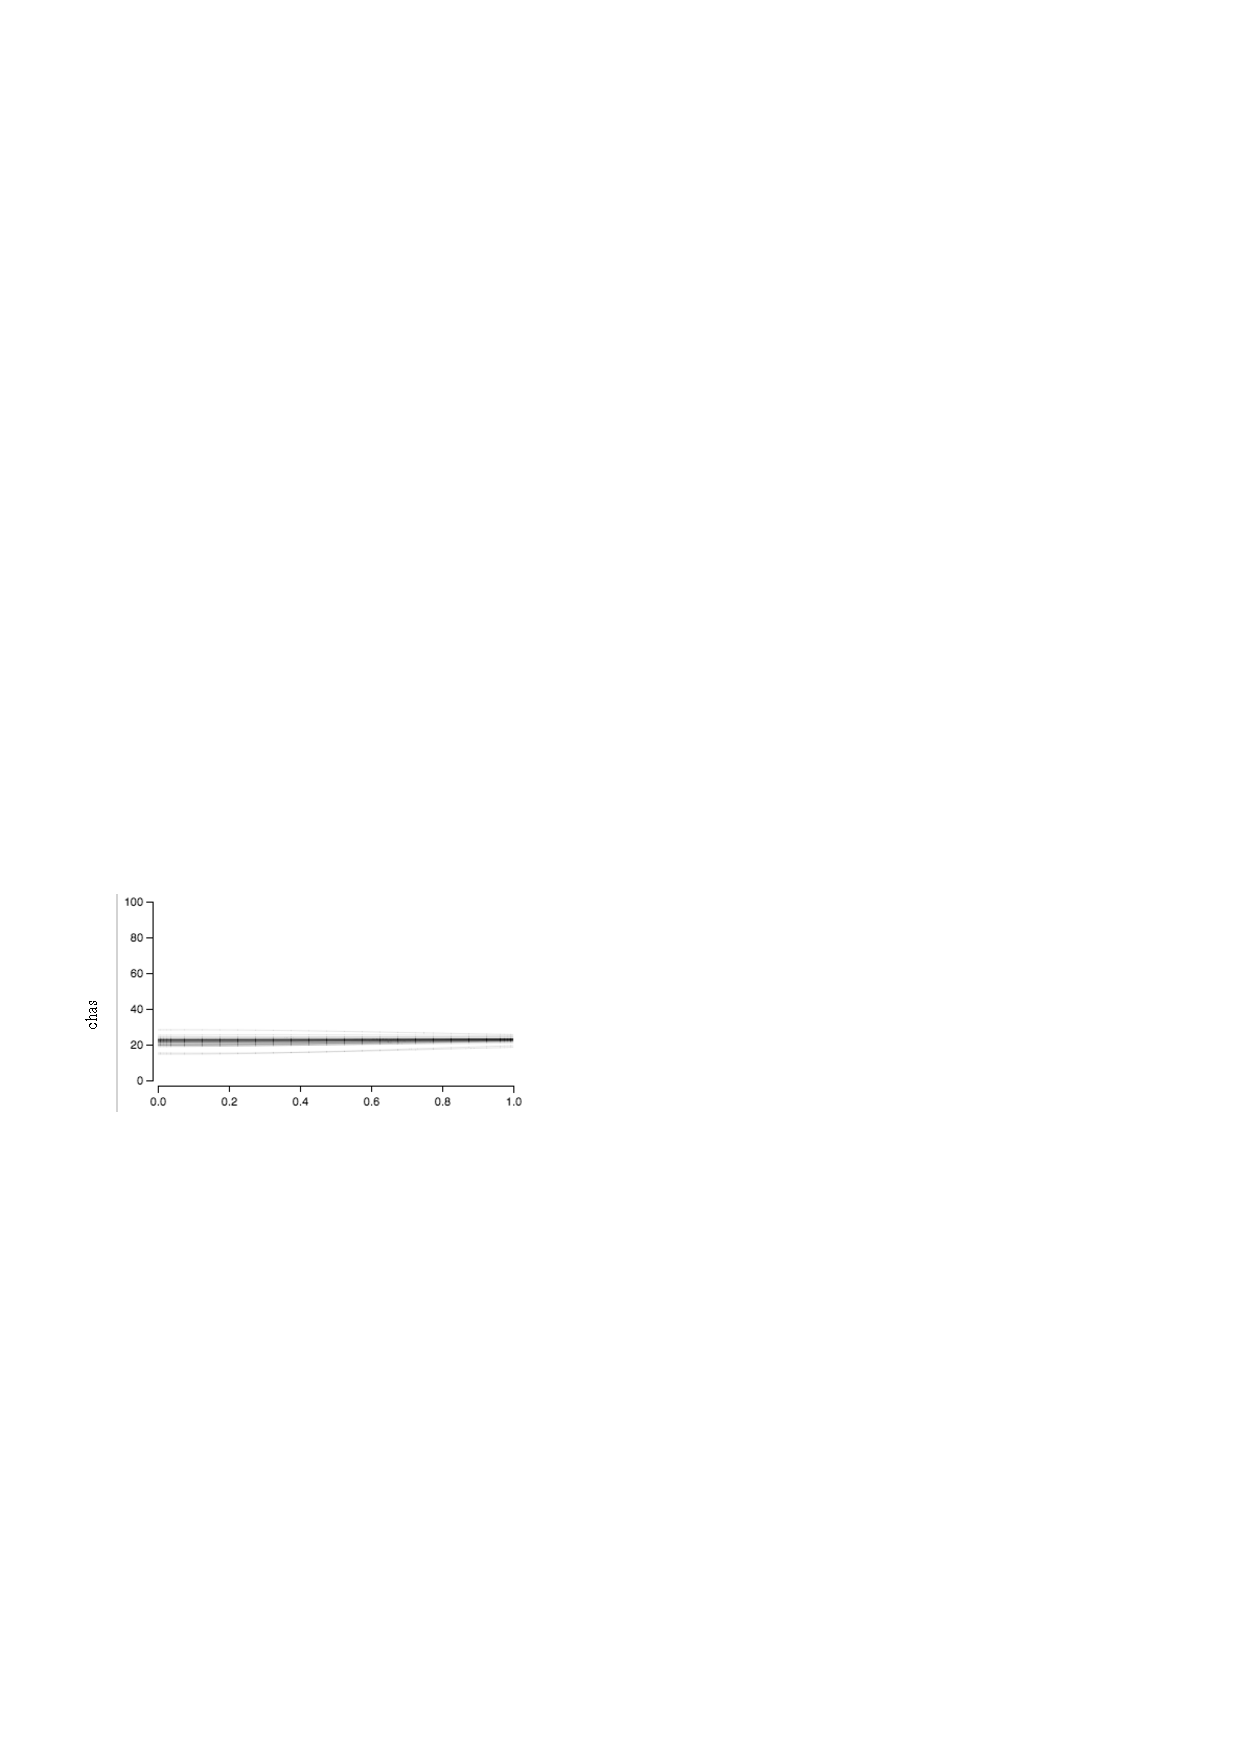
\includegraphics[width=0.1\textwidth]{svmr_4.pdf}
  \\
  \hline \\
  Nitric oxide concentration &
    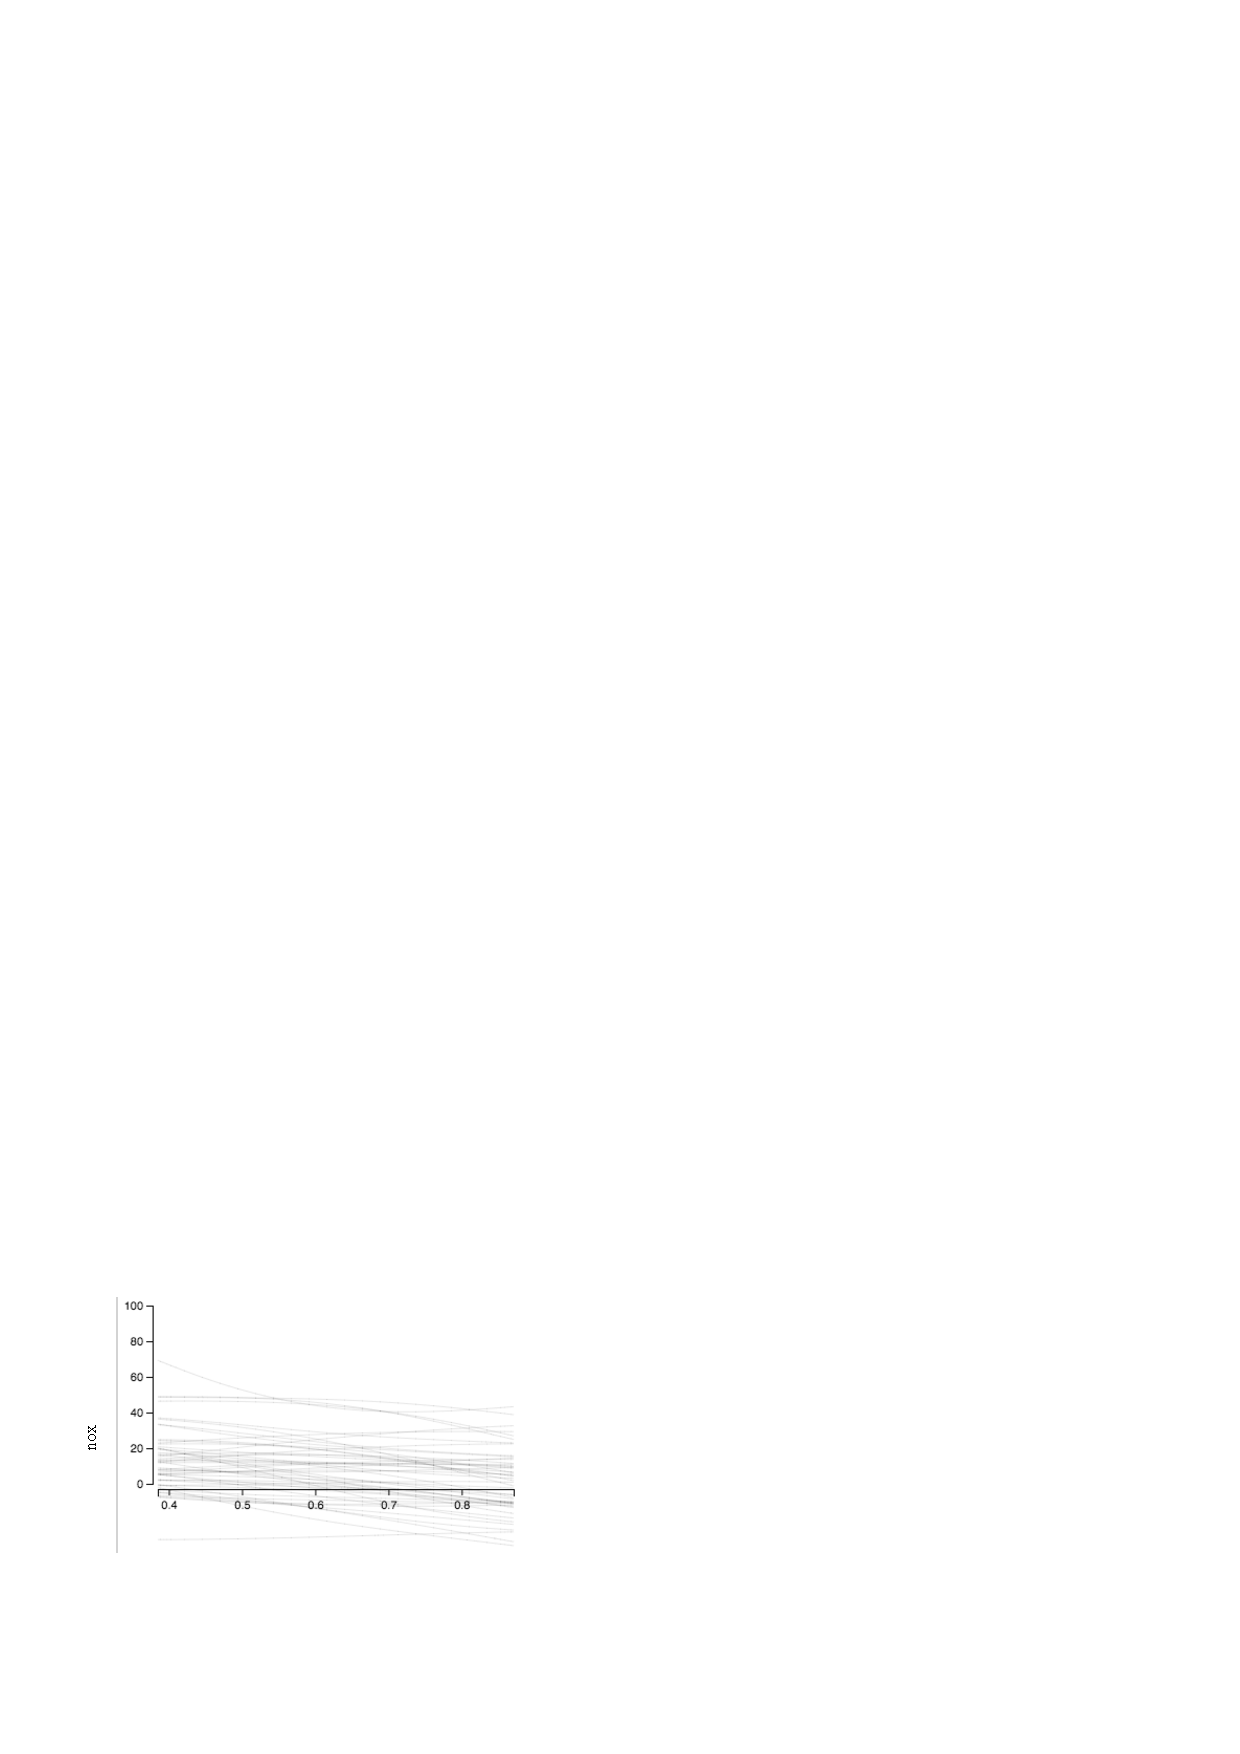
\includegraphics[width=0.1\textwidth]{nn26_5.pdf}
  &
    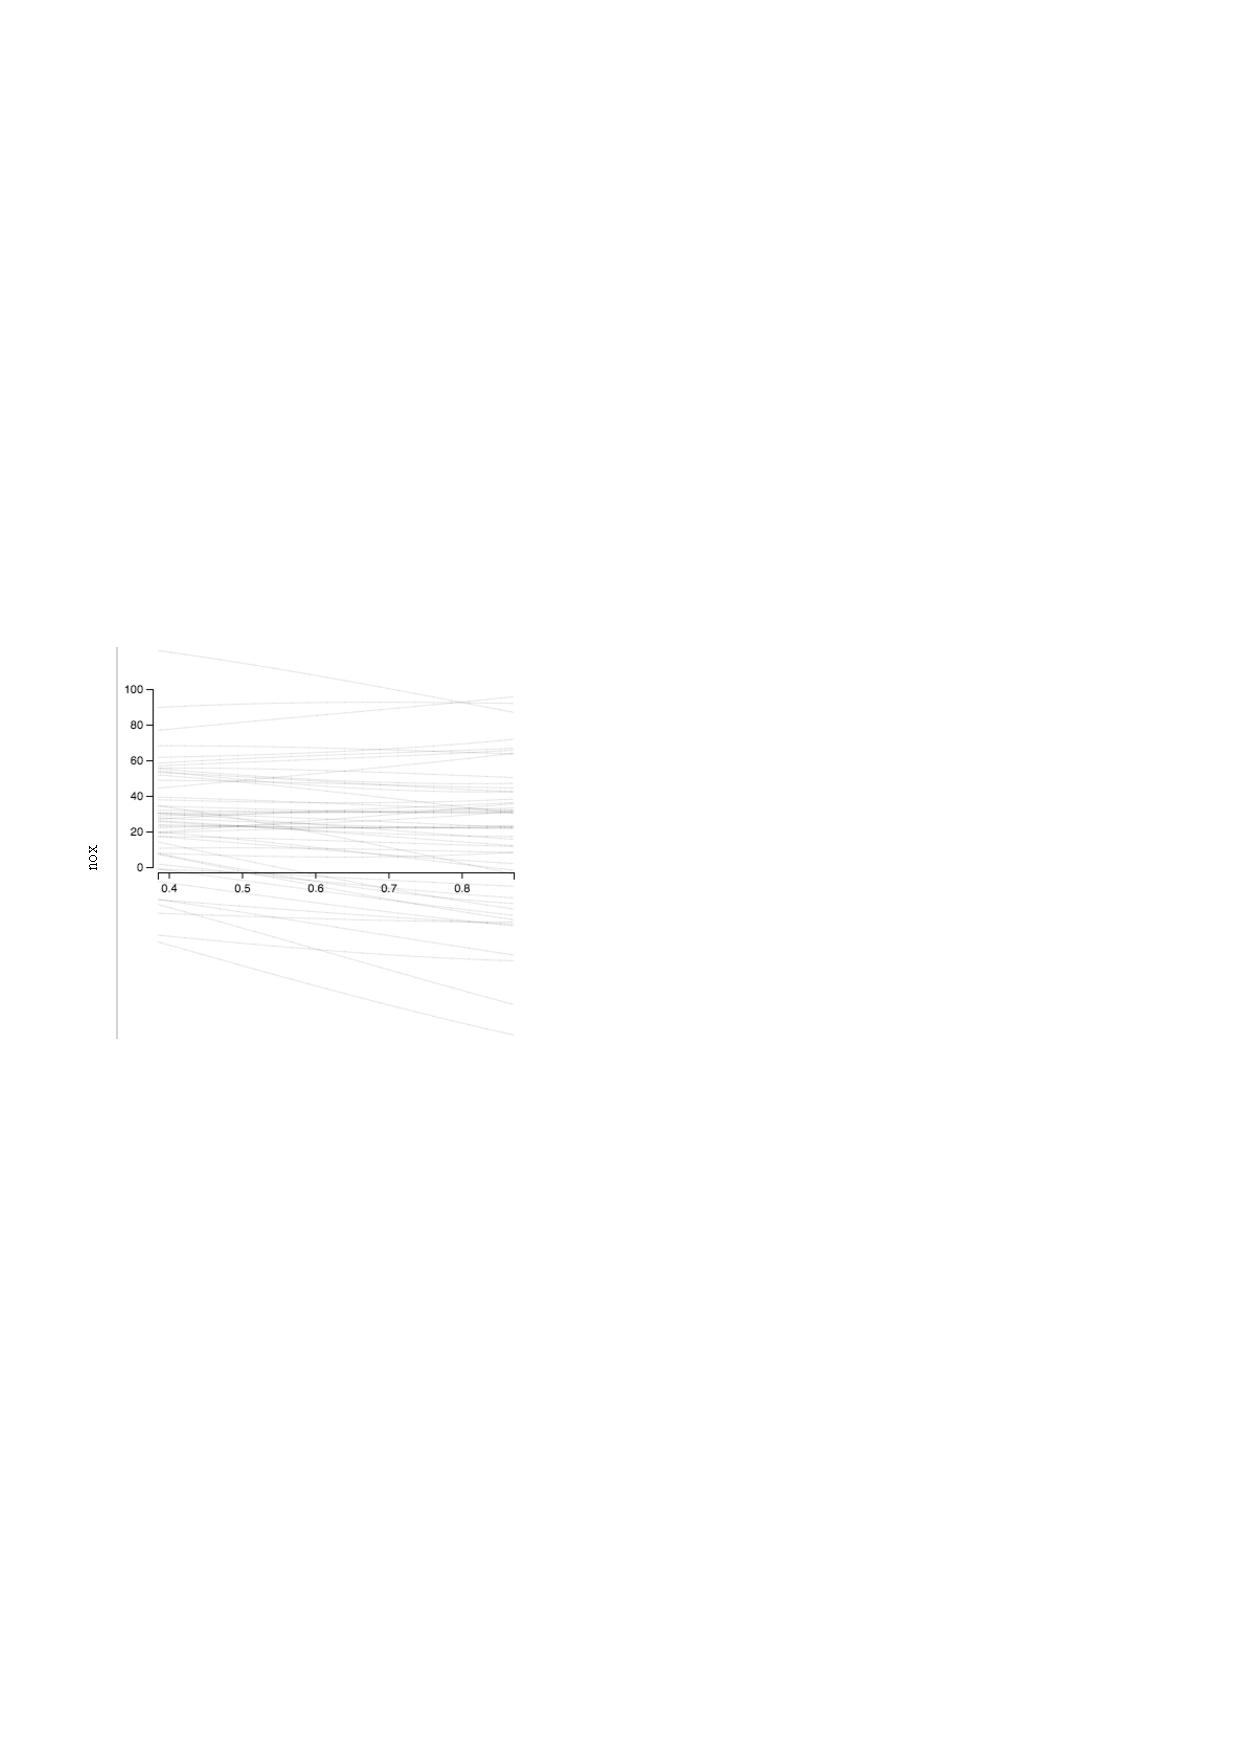
\includegraphics[width=0.1\textwidth]{svmp_5.pdf}
  &
    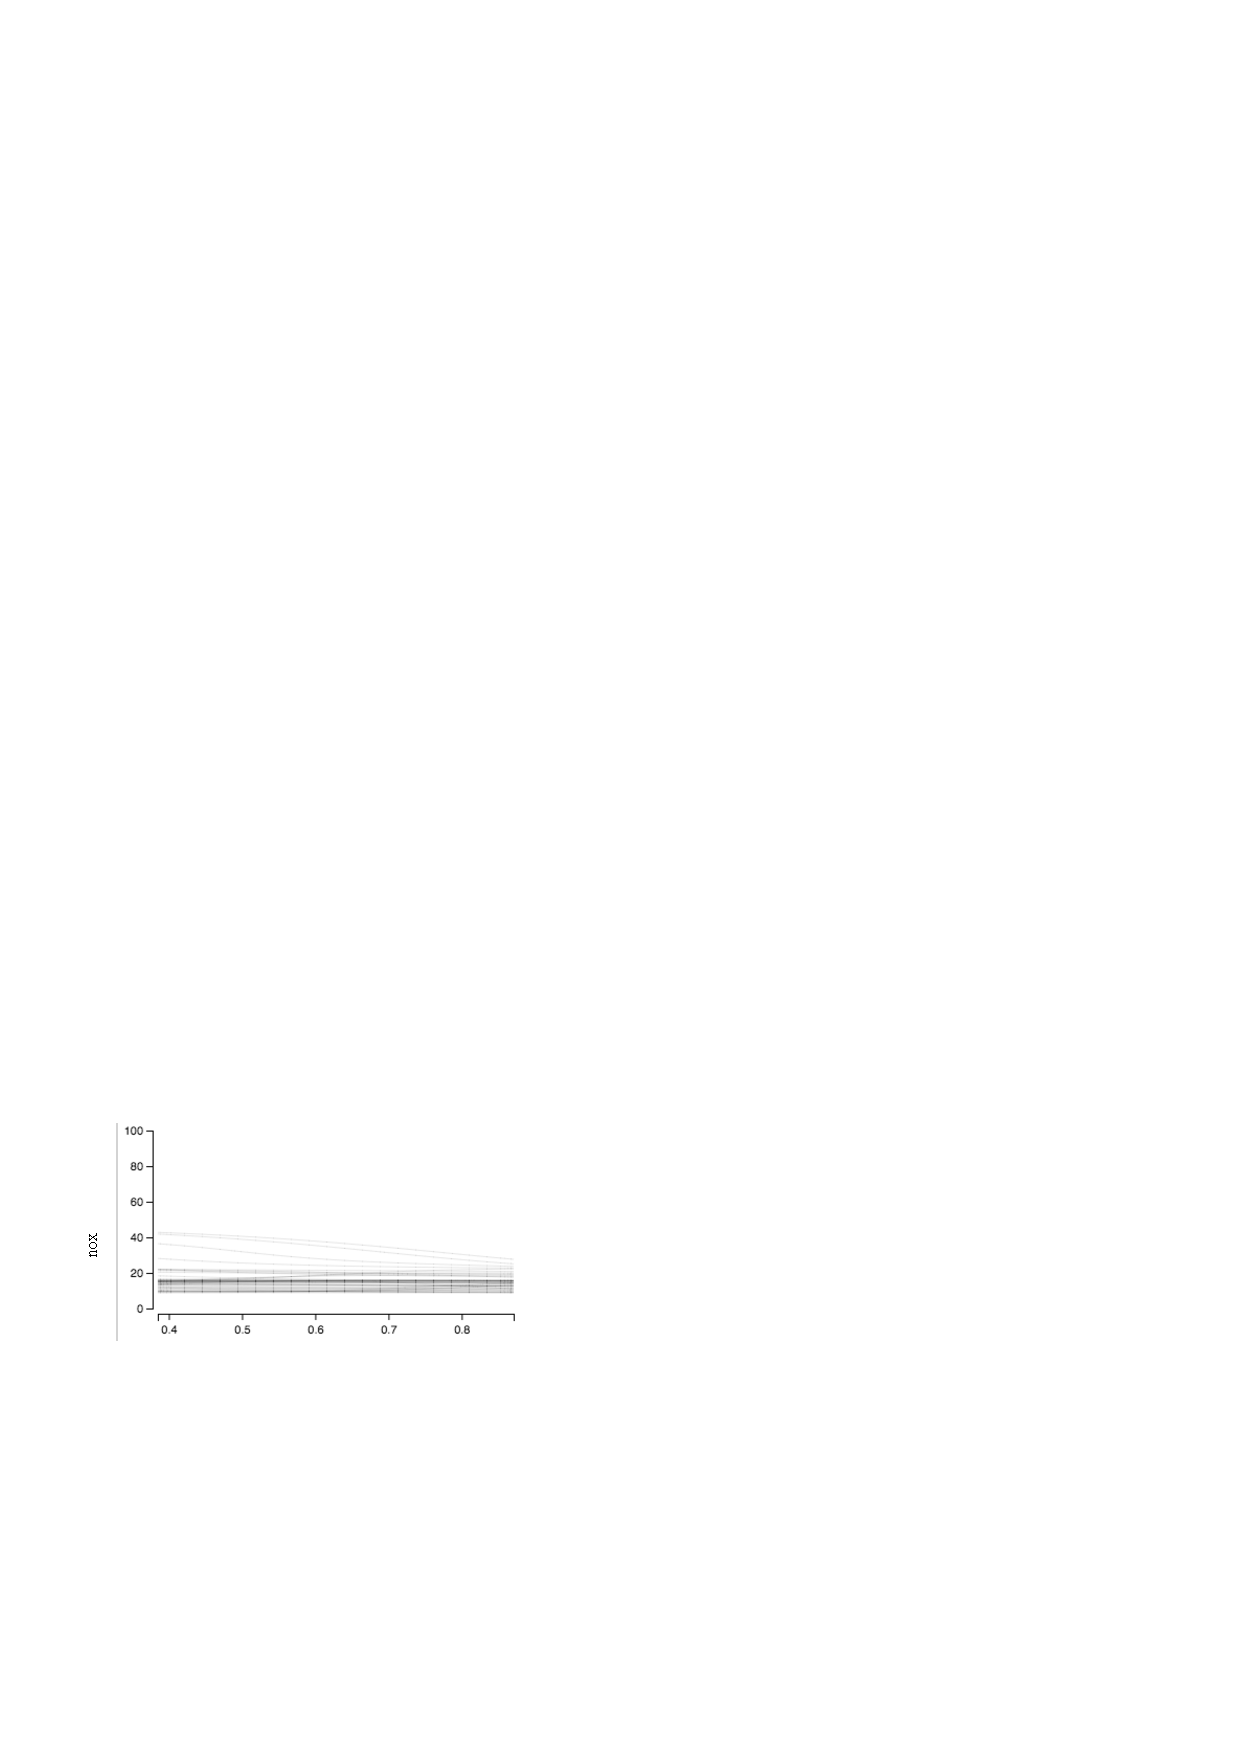
\includegraphics[width=0.1\textwidth]{nn5x3_5.pdf}
  &
    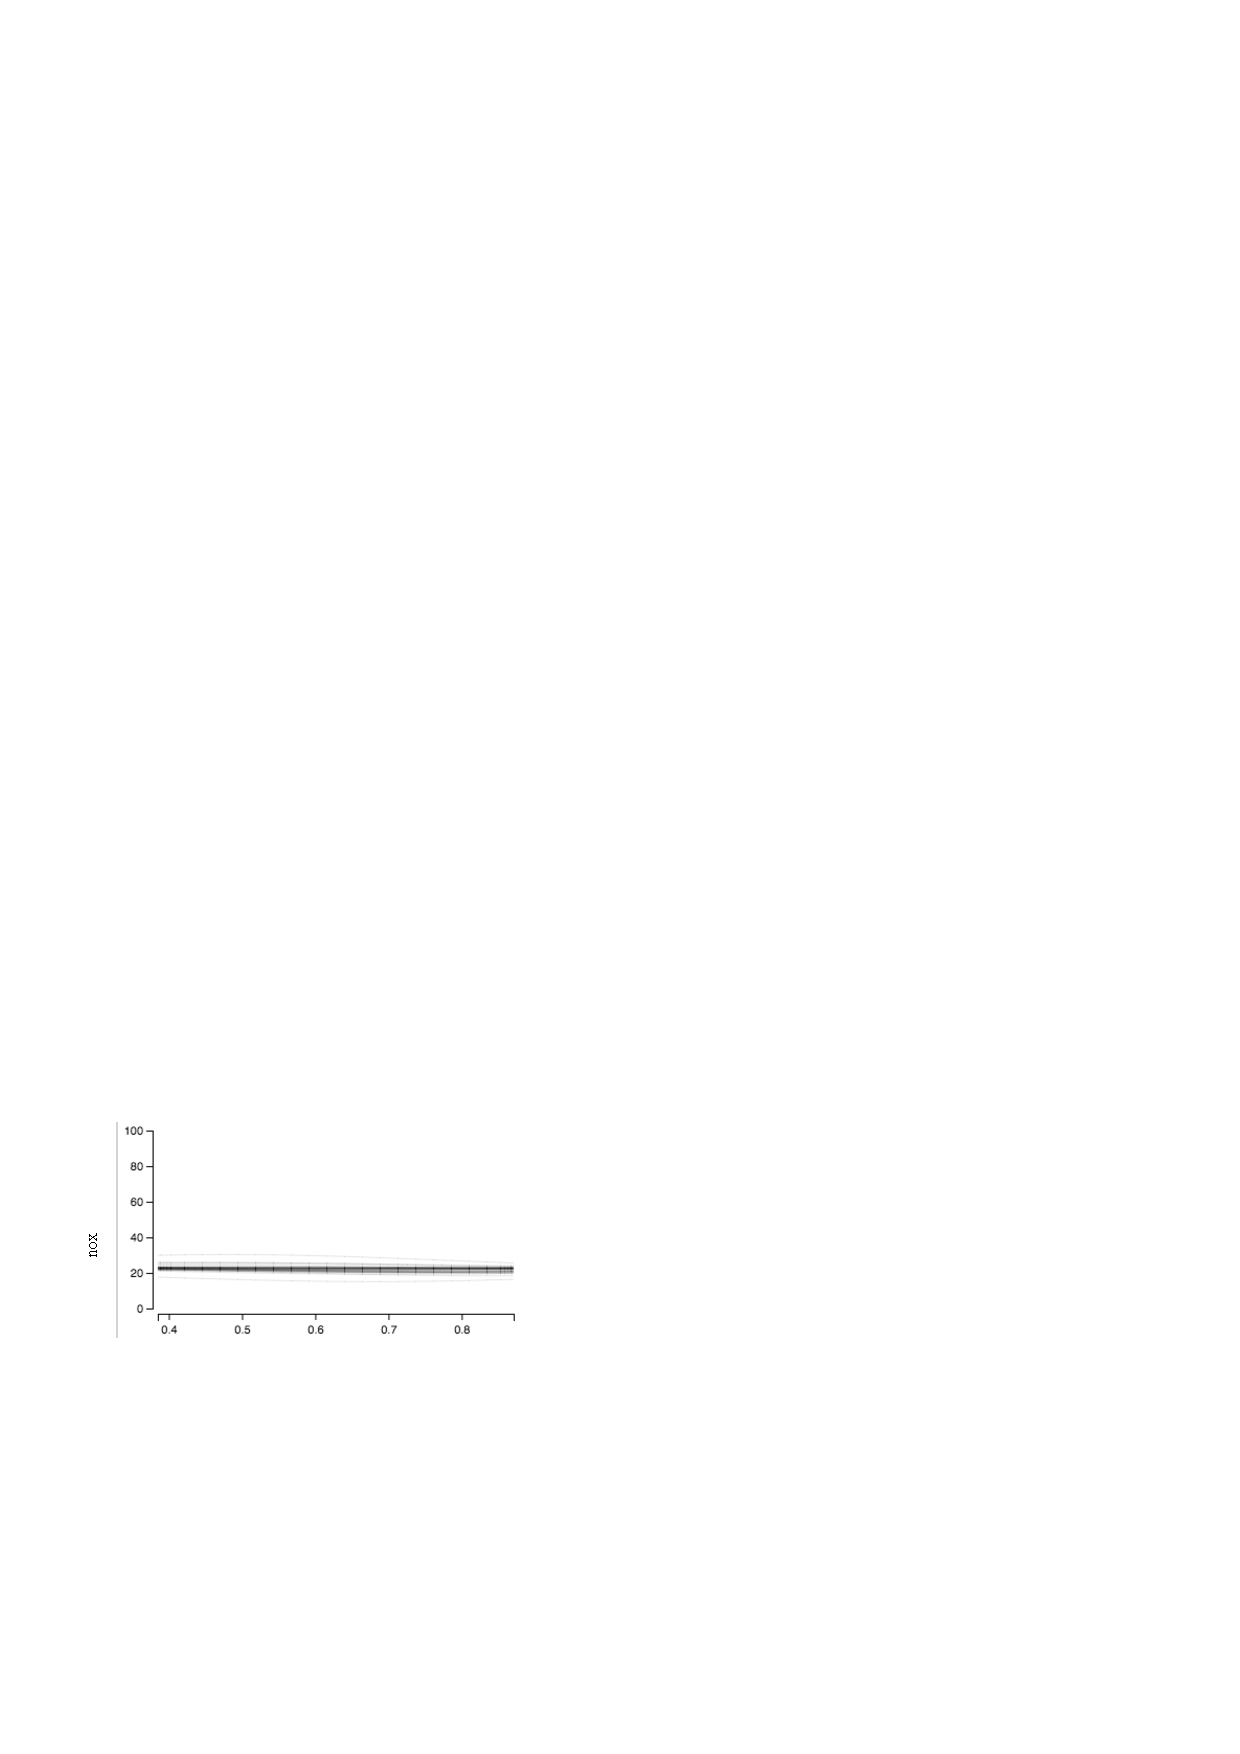
\includegraphics[width=0.1\textwidth]{svmr_5.pdf}
  \\
  \hline \\
  Average number of rooms per dwelling &
    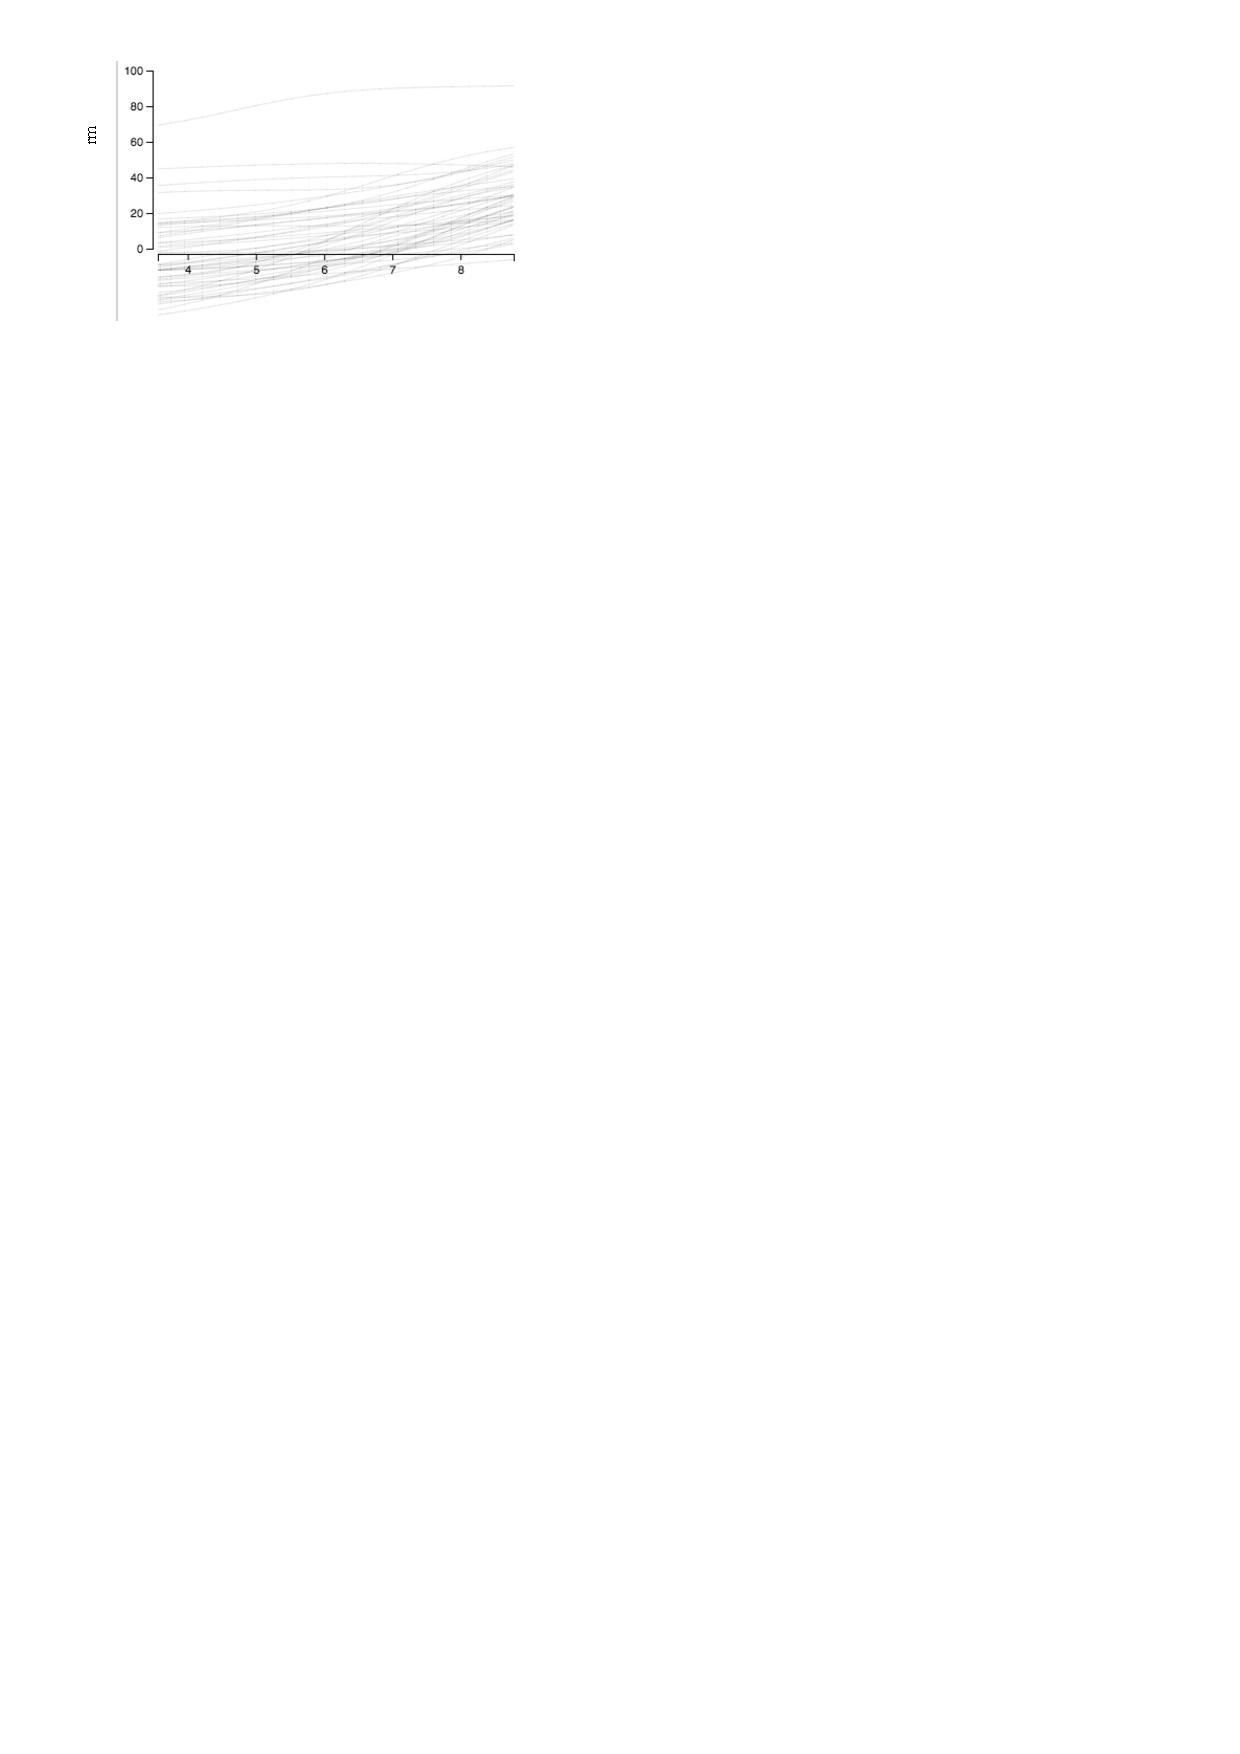
\includegraphics[width=0.1\textwidth]{nn26_6.pdf}
  &
    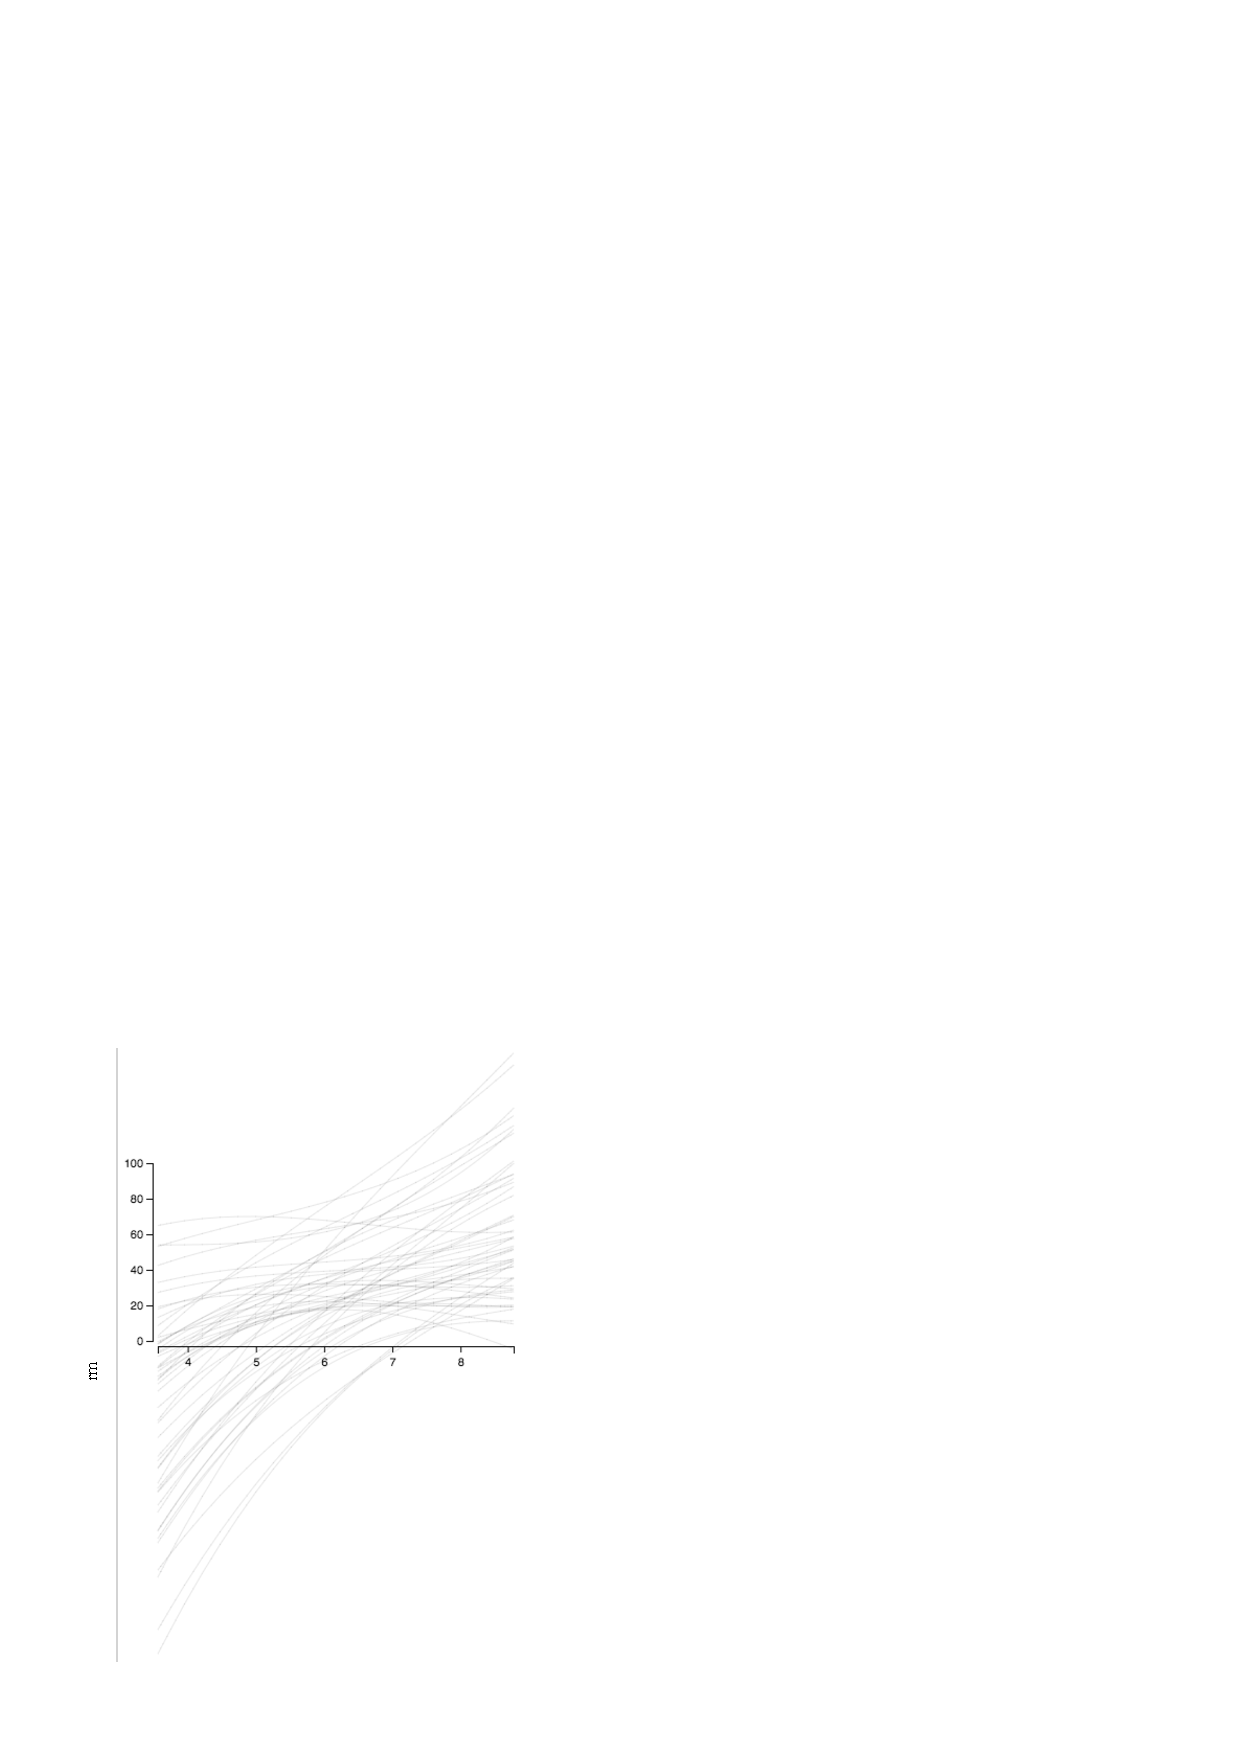
\includegraphics[width=0.1\textwidth]{svmp_6.pdf}
  &
    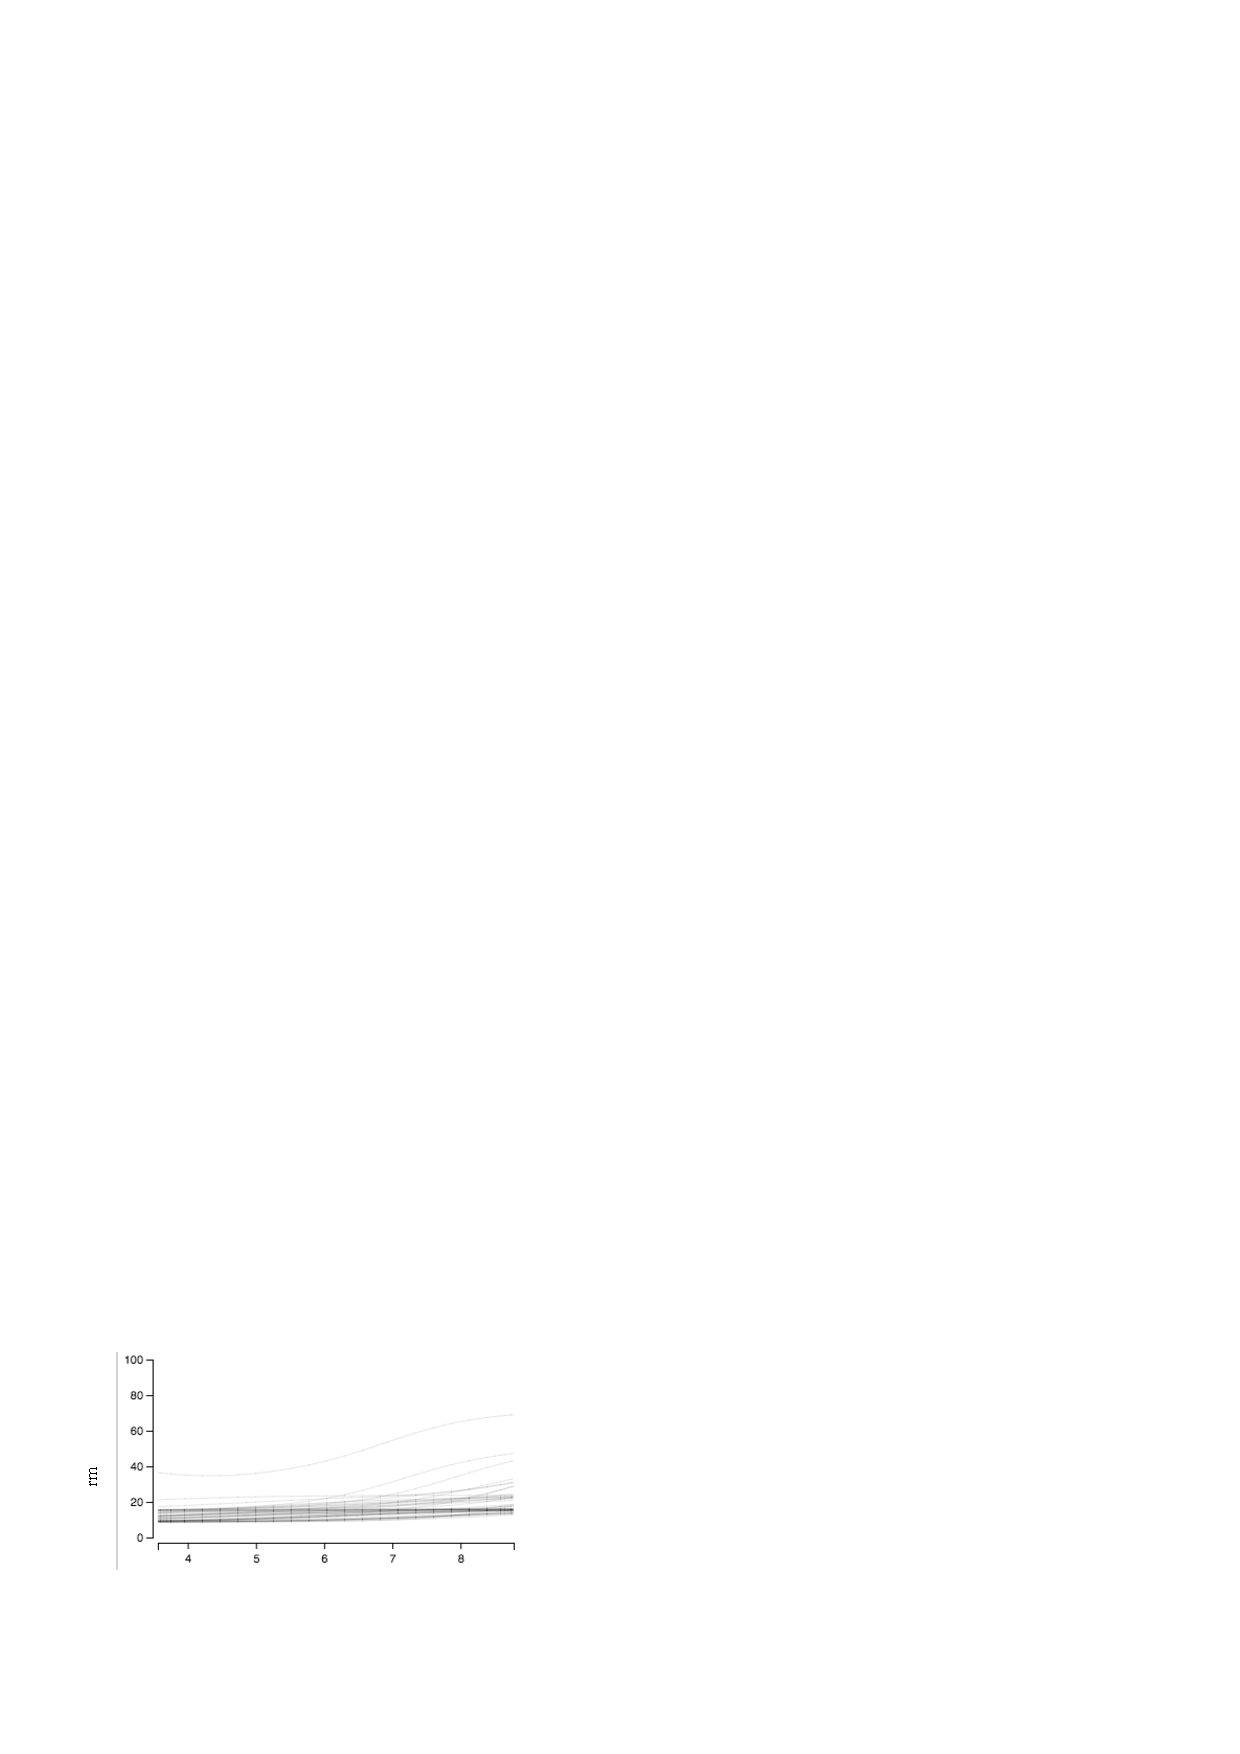
\includegraphics[width=0.1\textwidth]{nn5x3_6.pdf}
  &
    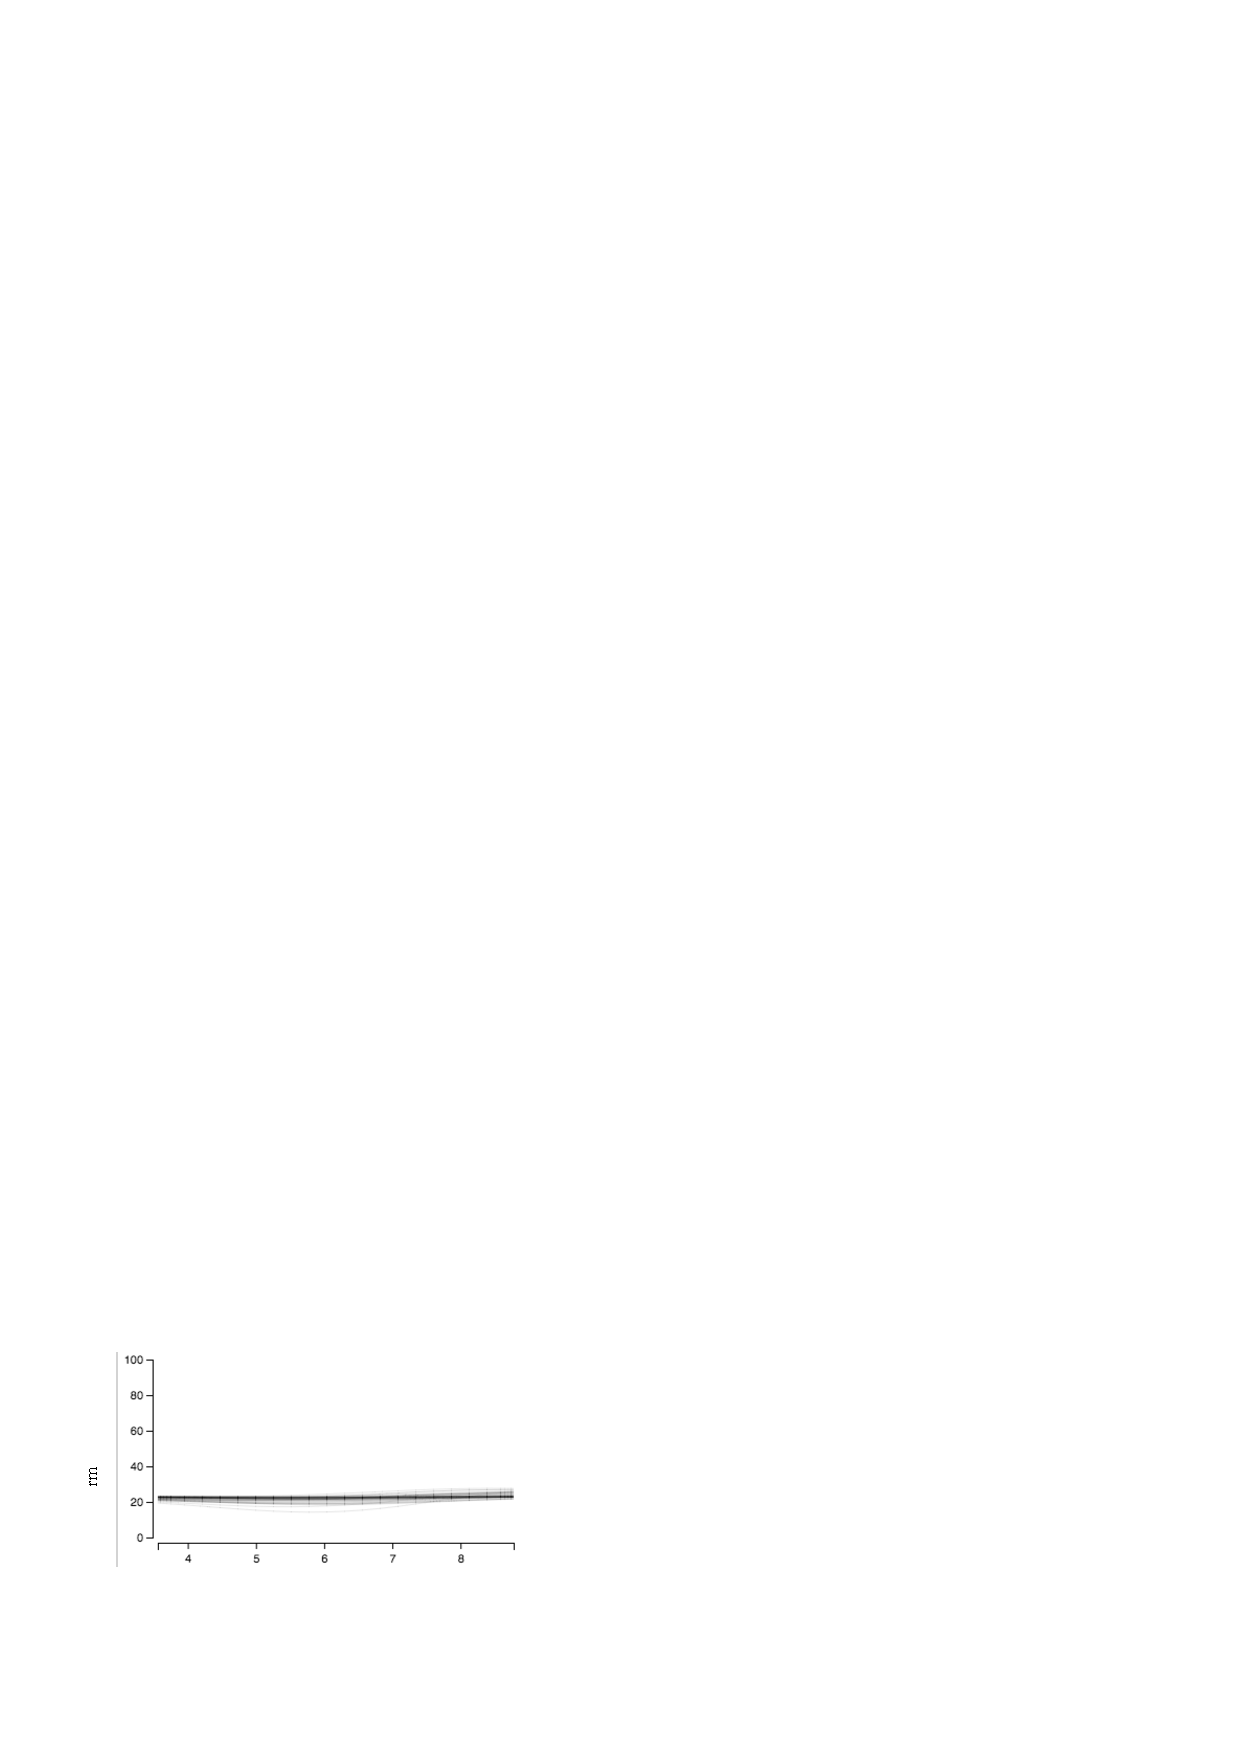
\includegraphics[width=0.1\textwidth]{svmr_6.pdf}
  \\
  \hline \\
  Units built prior to 1940 &
    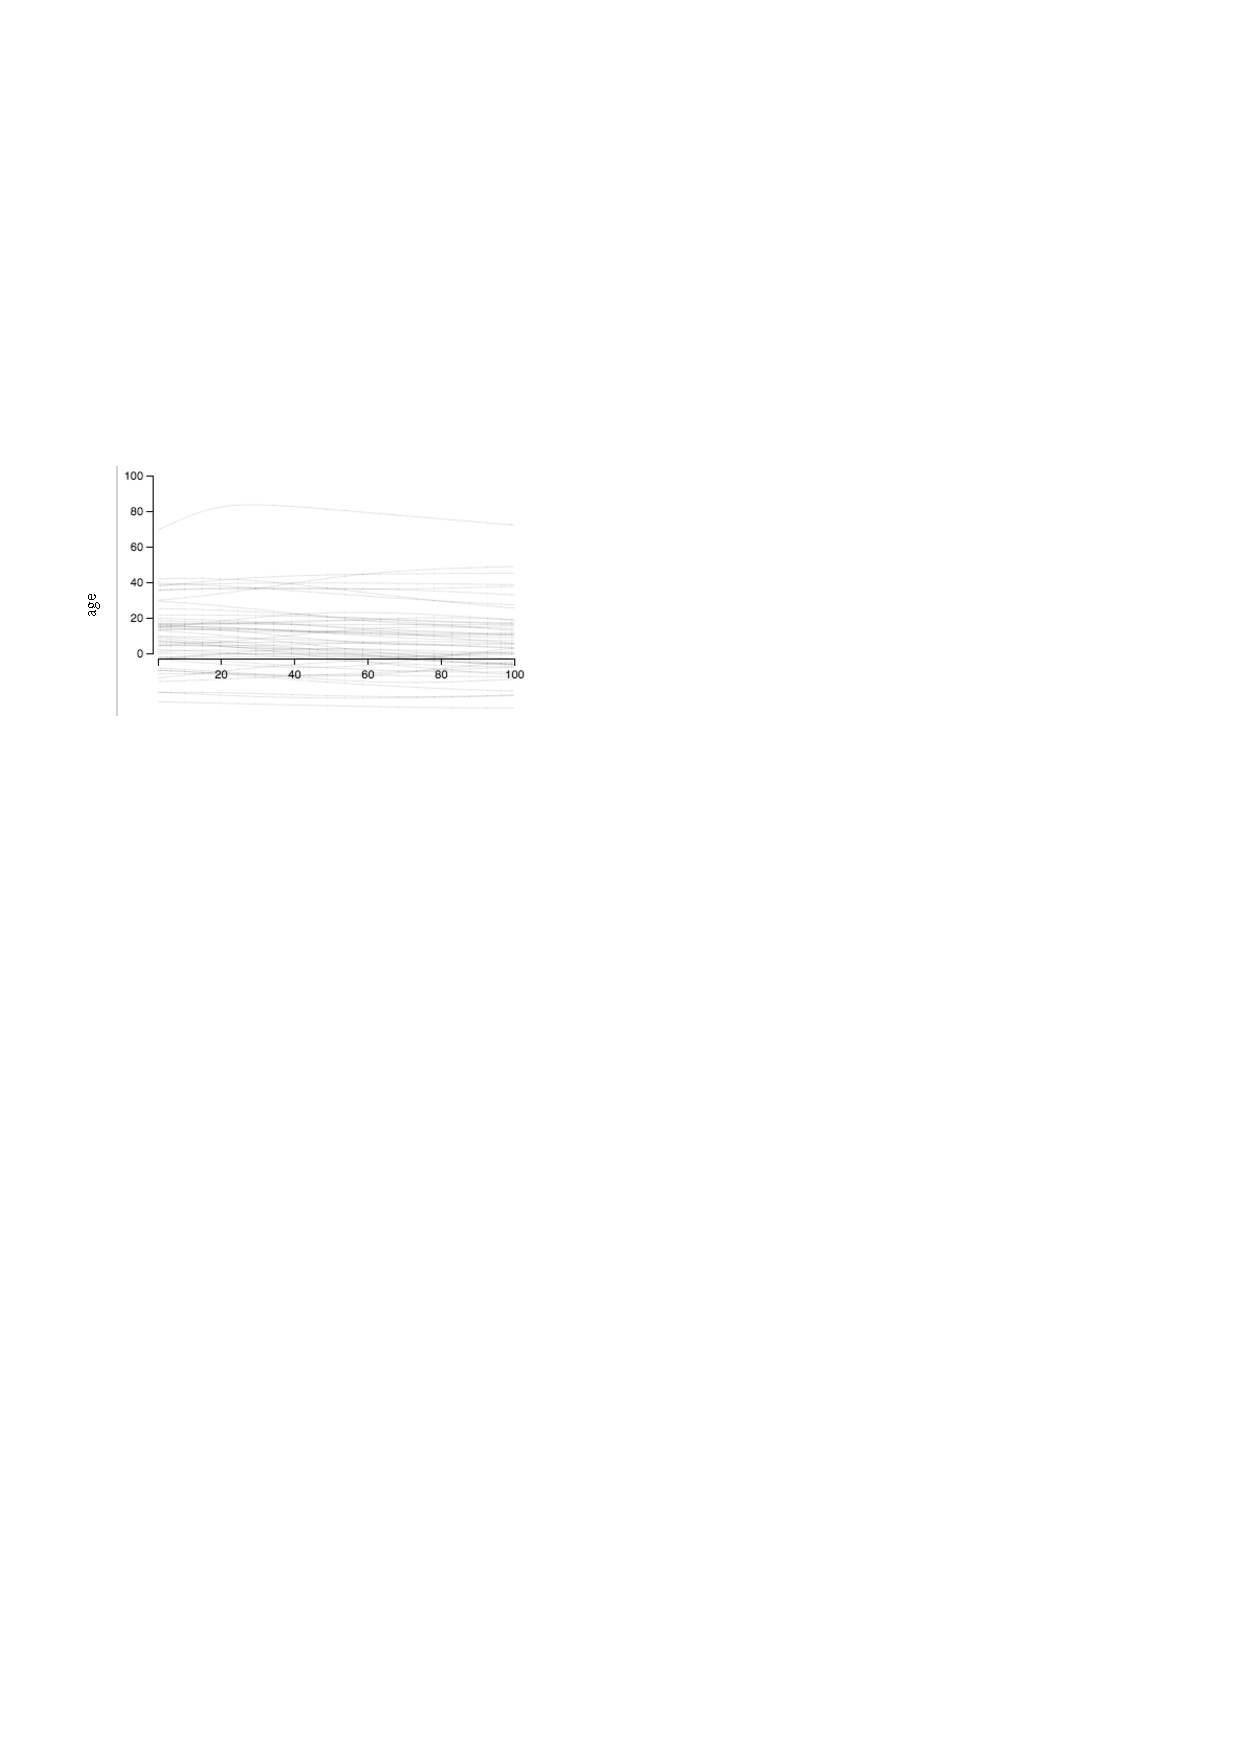
\includegraphics[width=0.1\textwidth]{nn26_7.pdf}
  &
    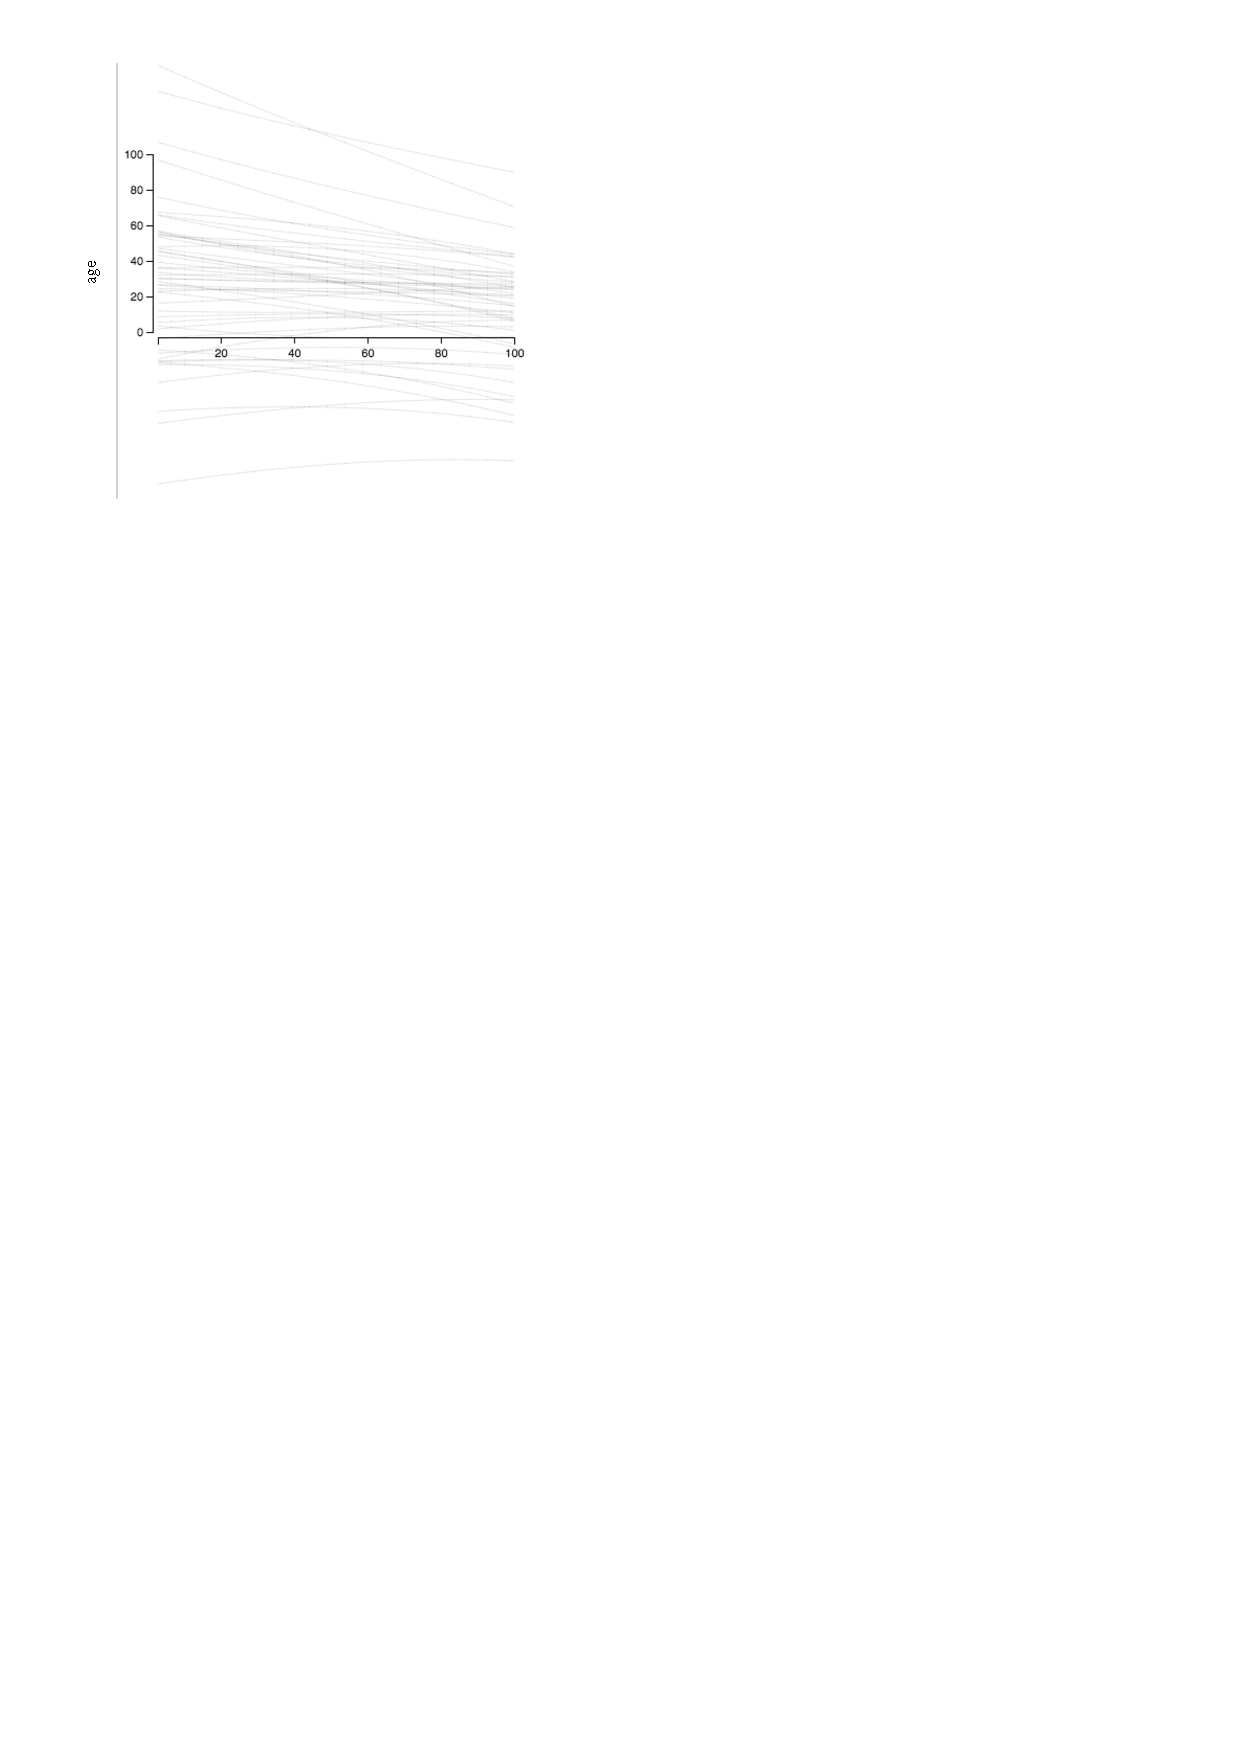
\includegraphics[width=0.1\textwidth]{svmp_7.pdf}
  &
    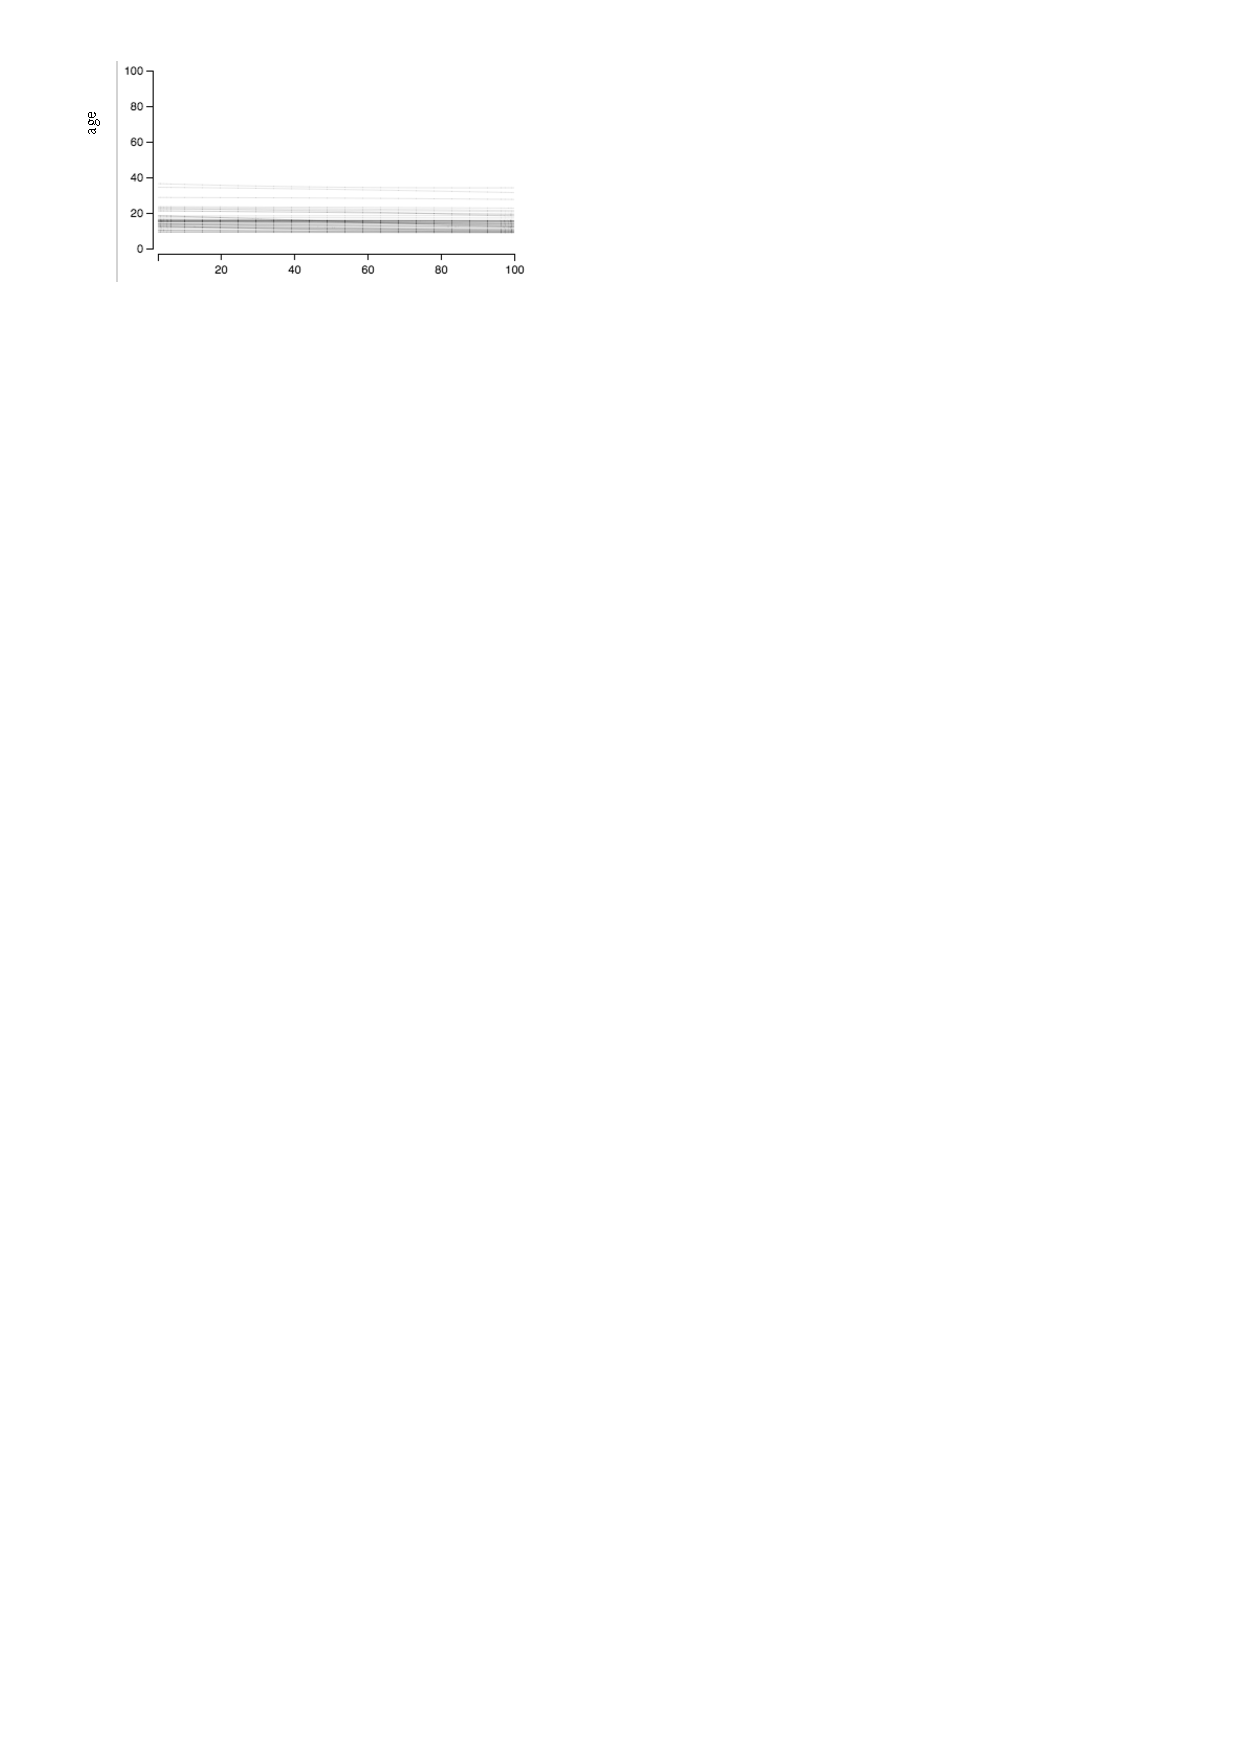
\includegraphics[width=0.1\textwidth]{nn5x3_7.pdf}
  &
    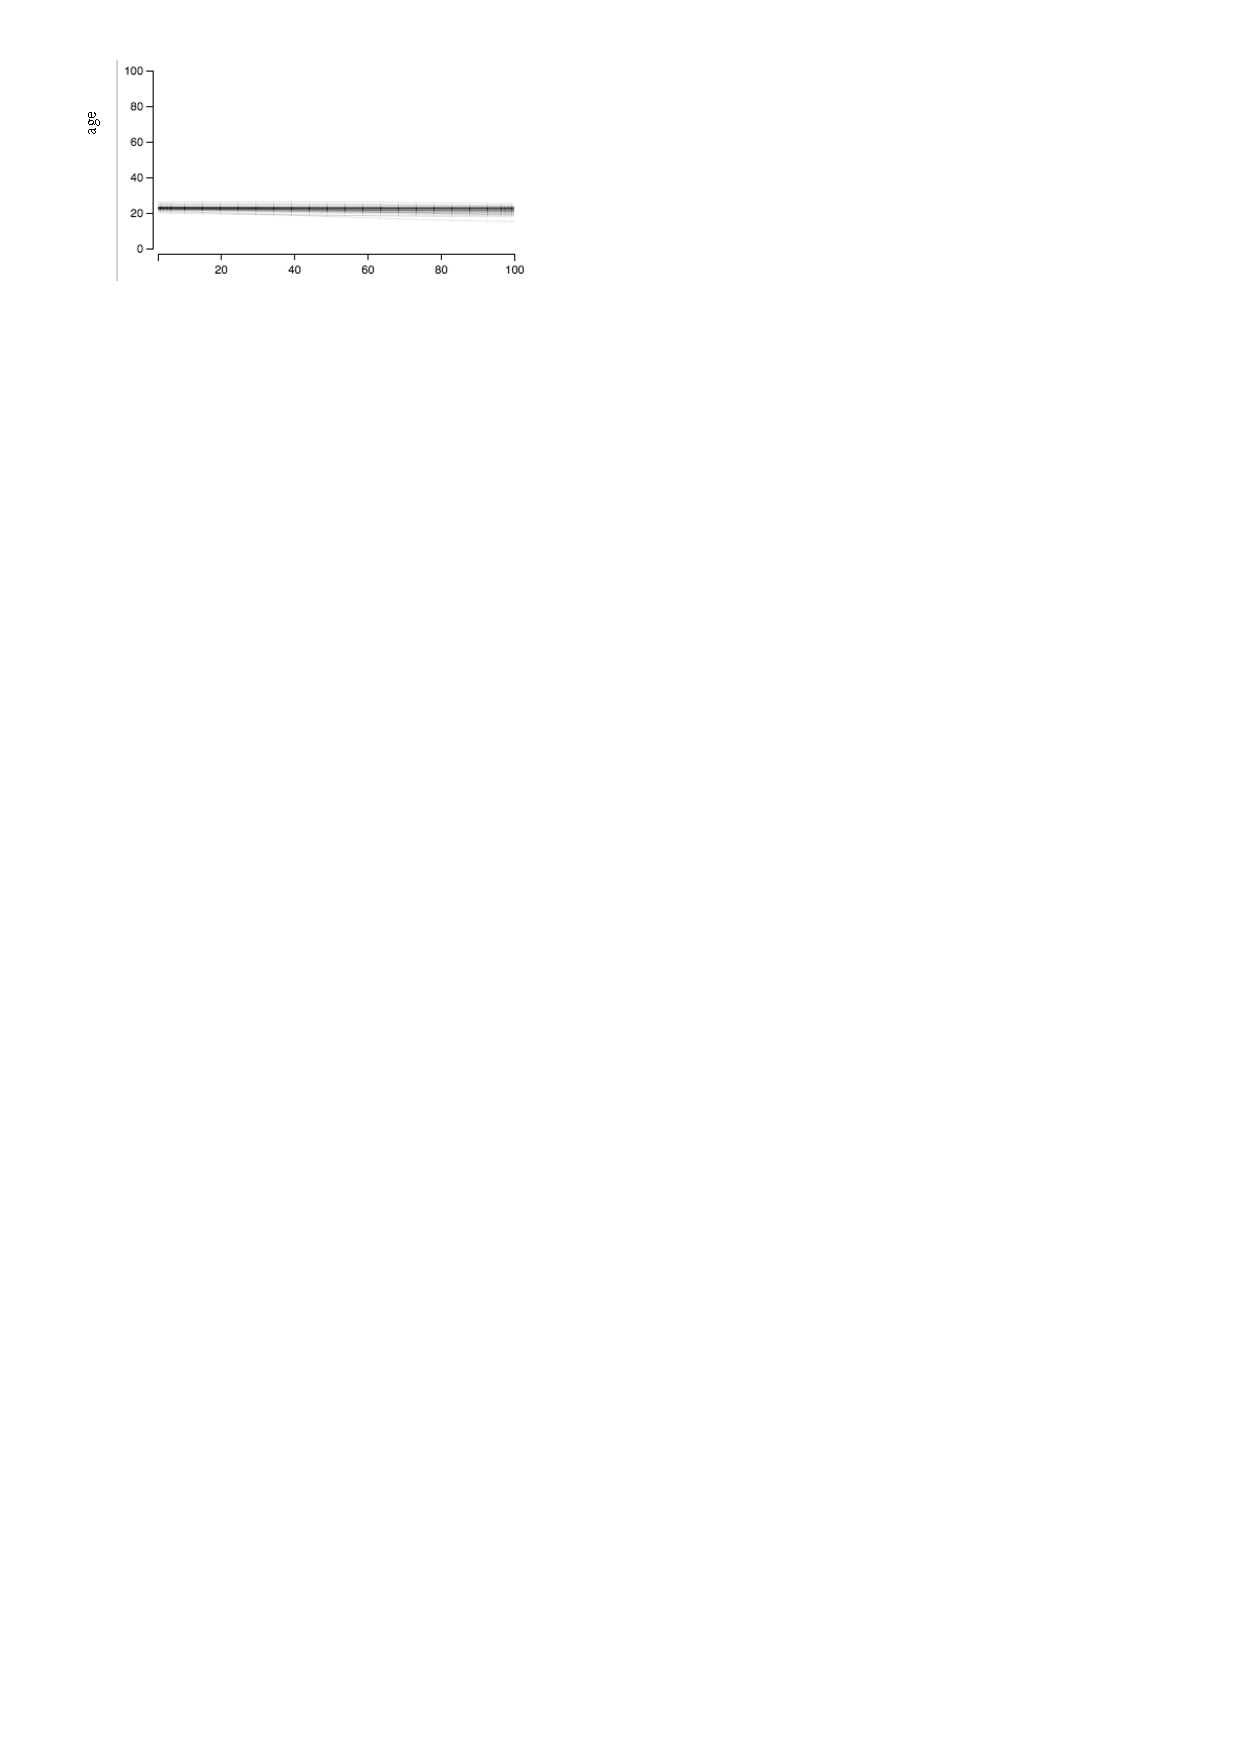
\includegraphics[width=0.1\textwidth]{svmr_7.pdf}
  \\
  \hline \\
  Distances to employment centres &
    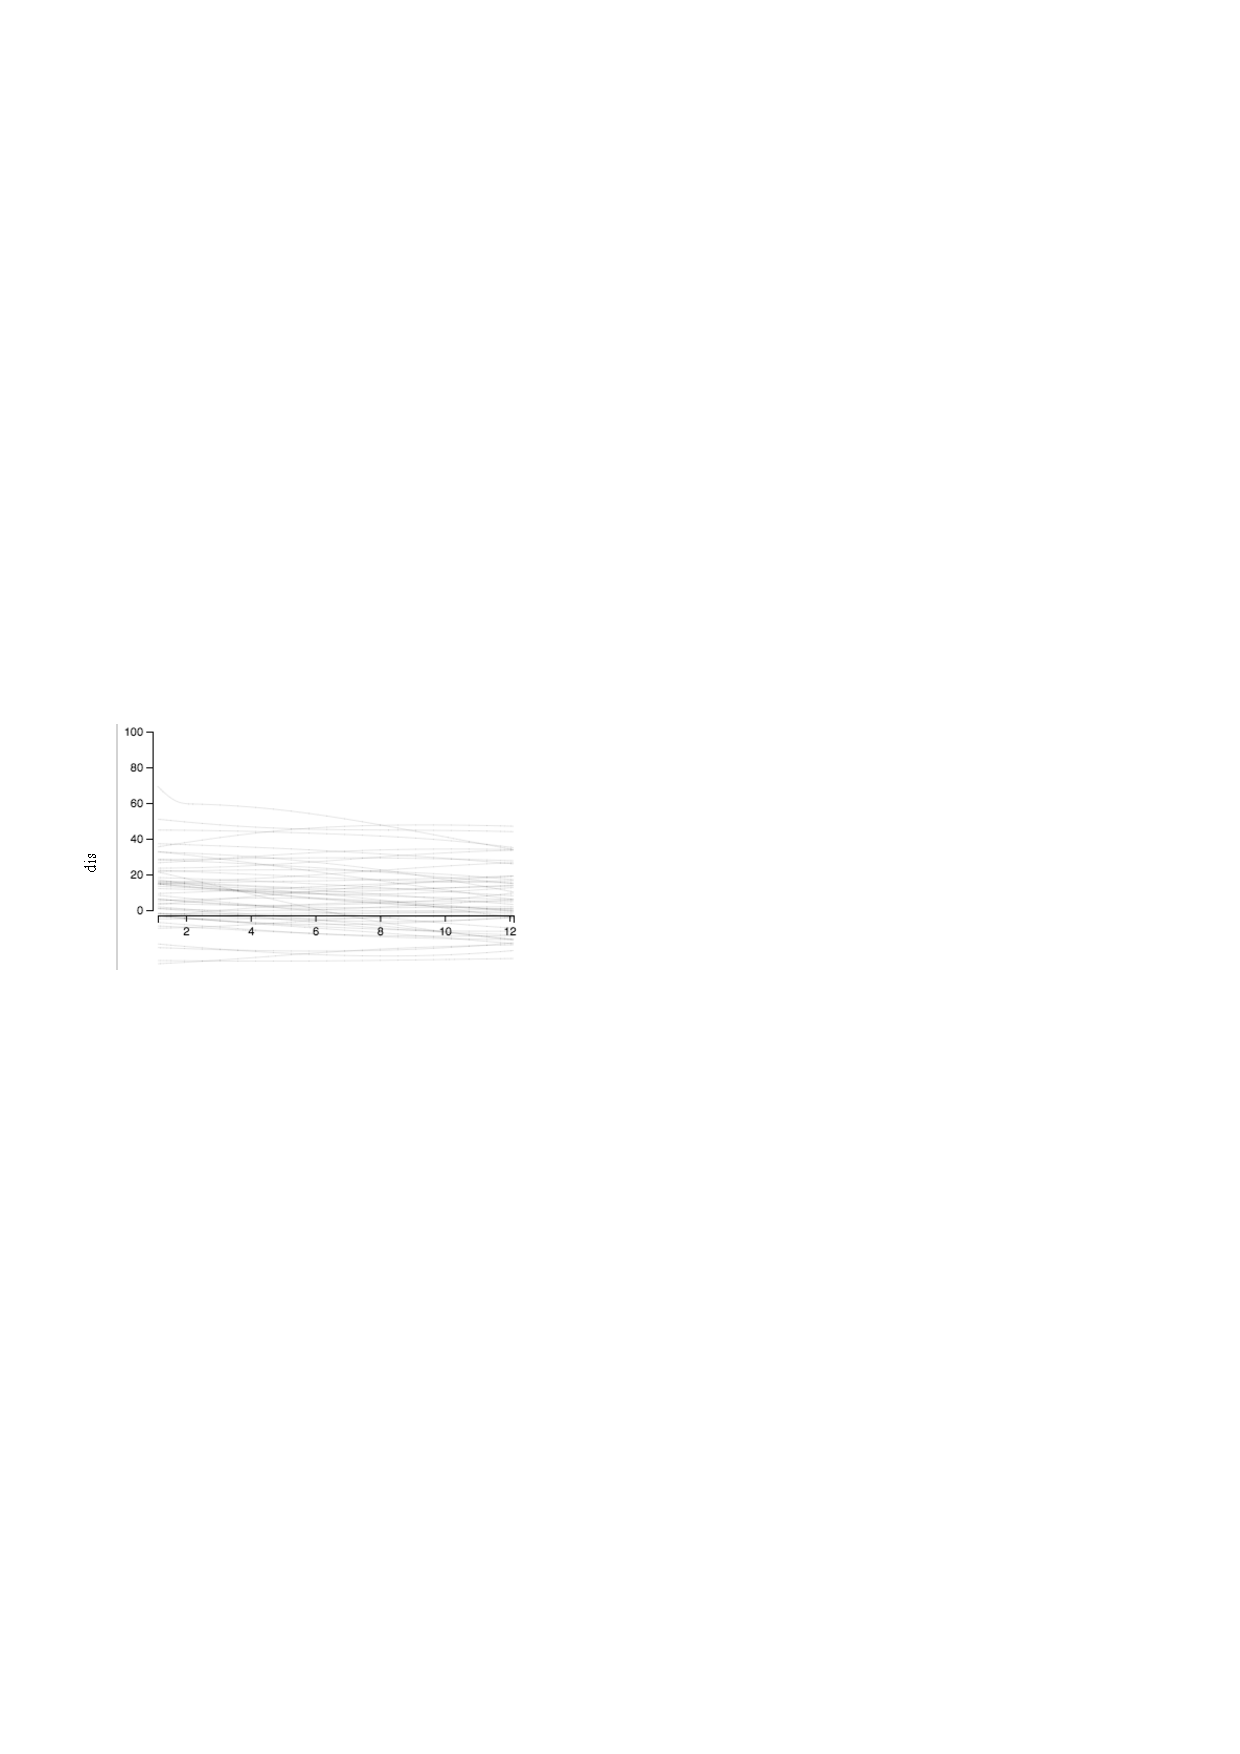
\includegraphics[width=0.1\textwidth]{nn26_8.pdf}
  &
    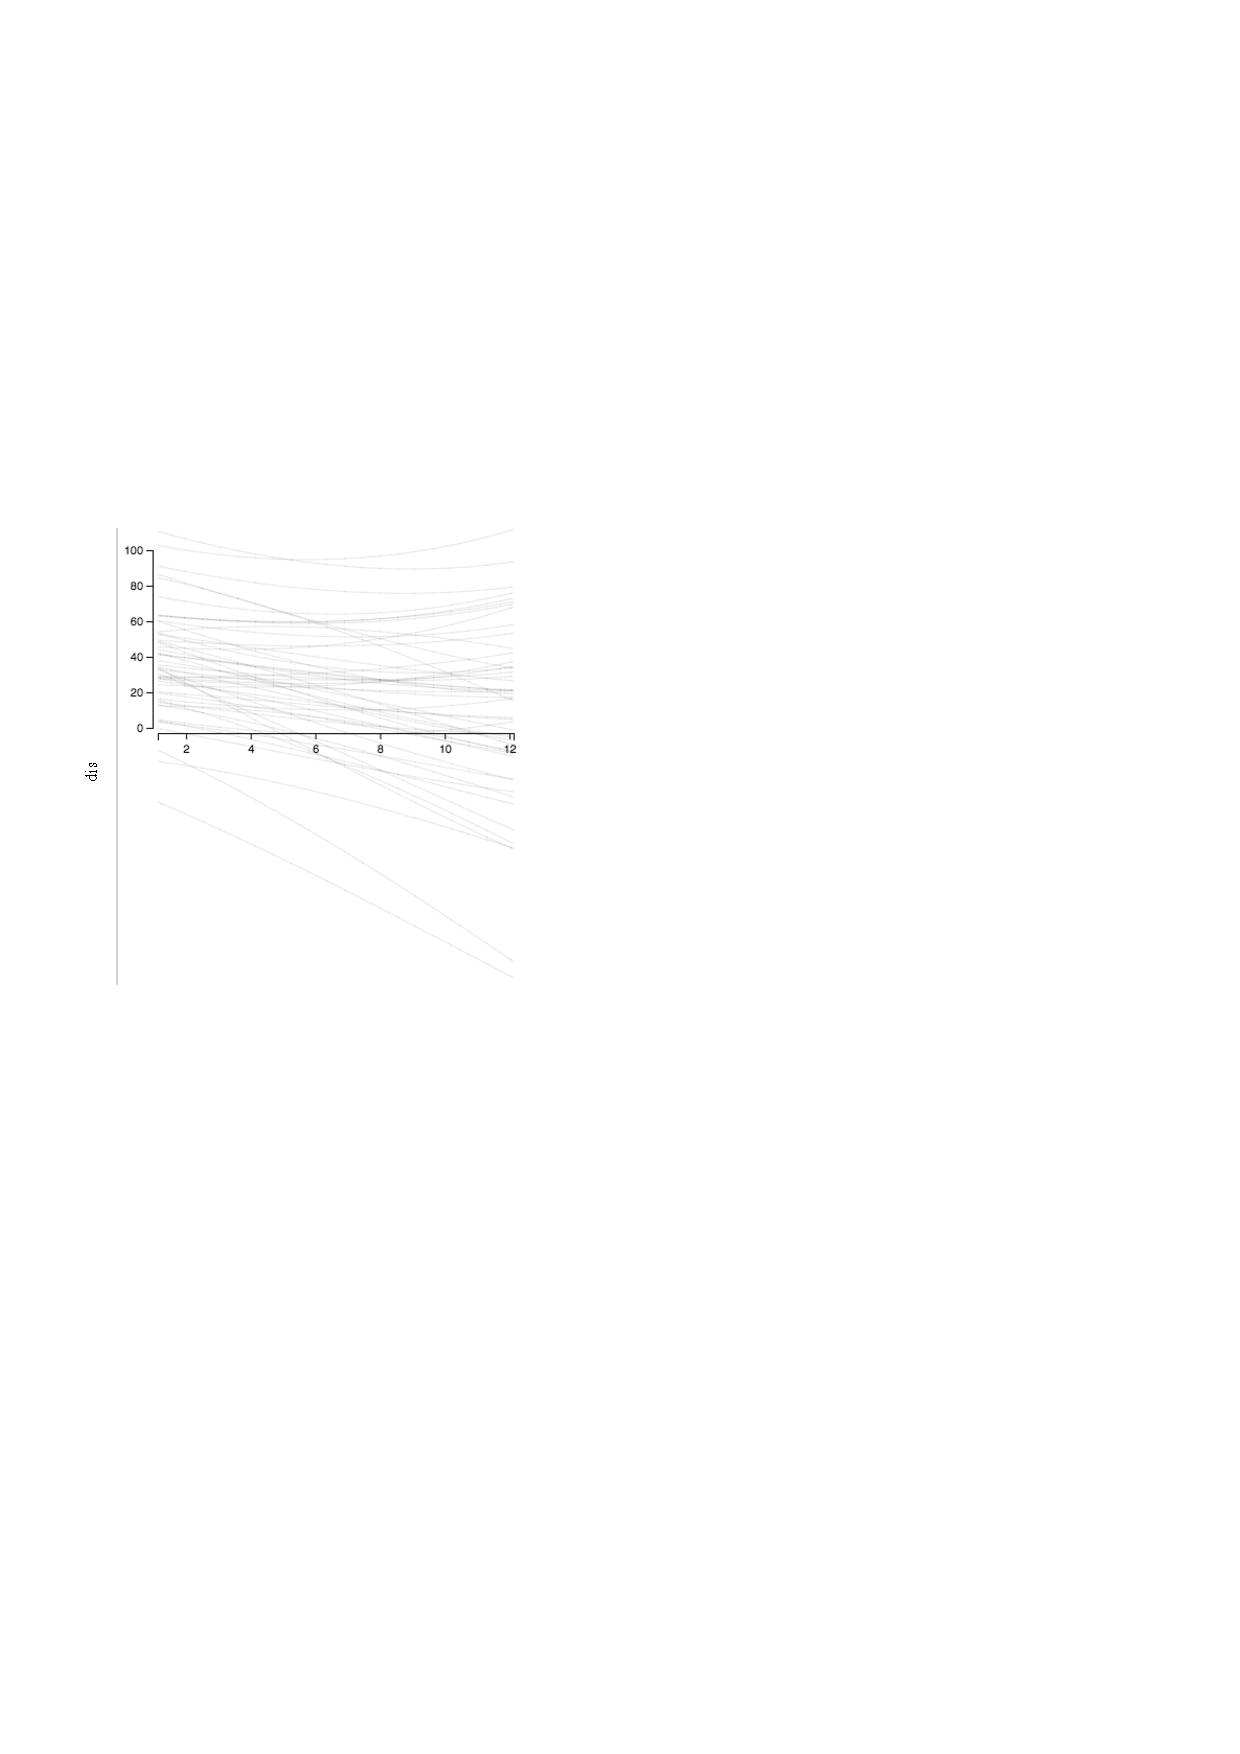
\includegraphics[width=0.1\textwidth]{svmp_8.pdf}
  &
    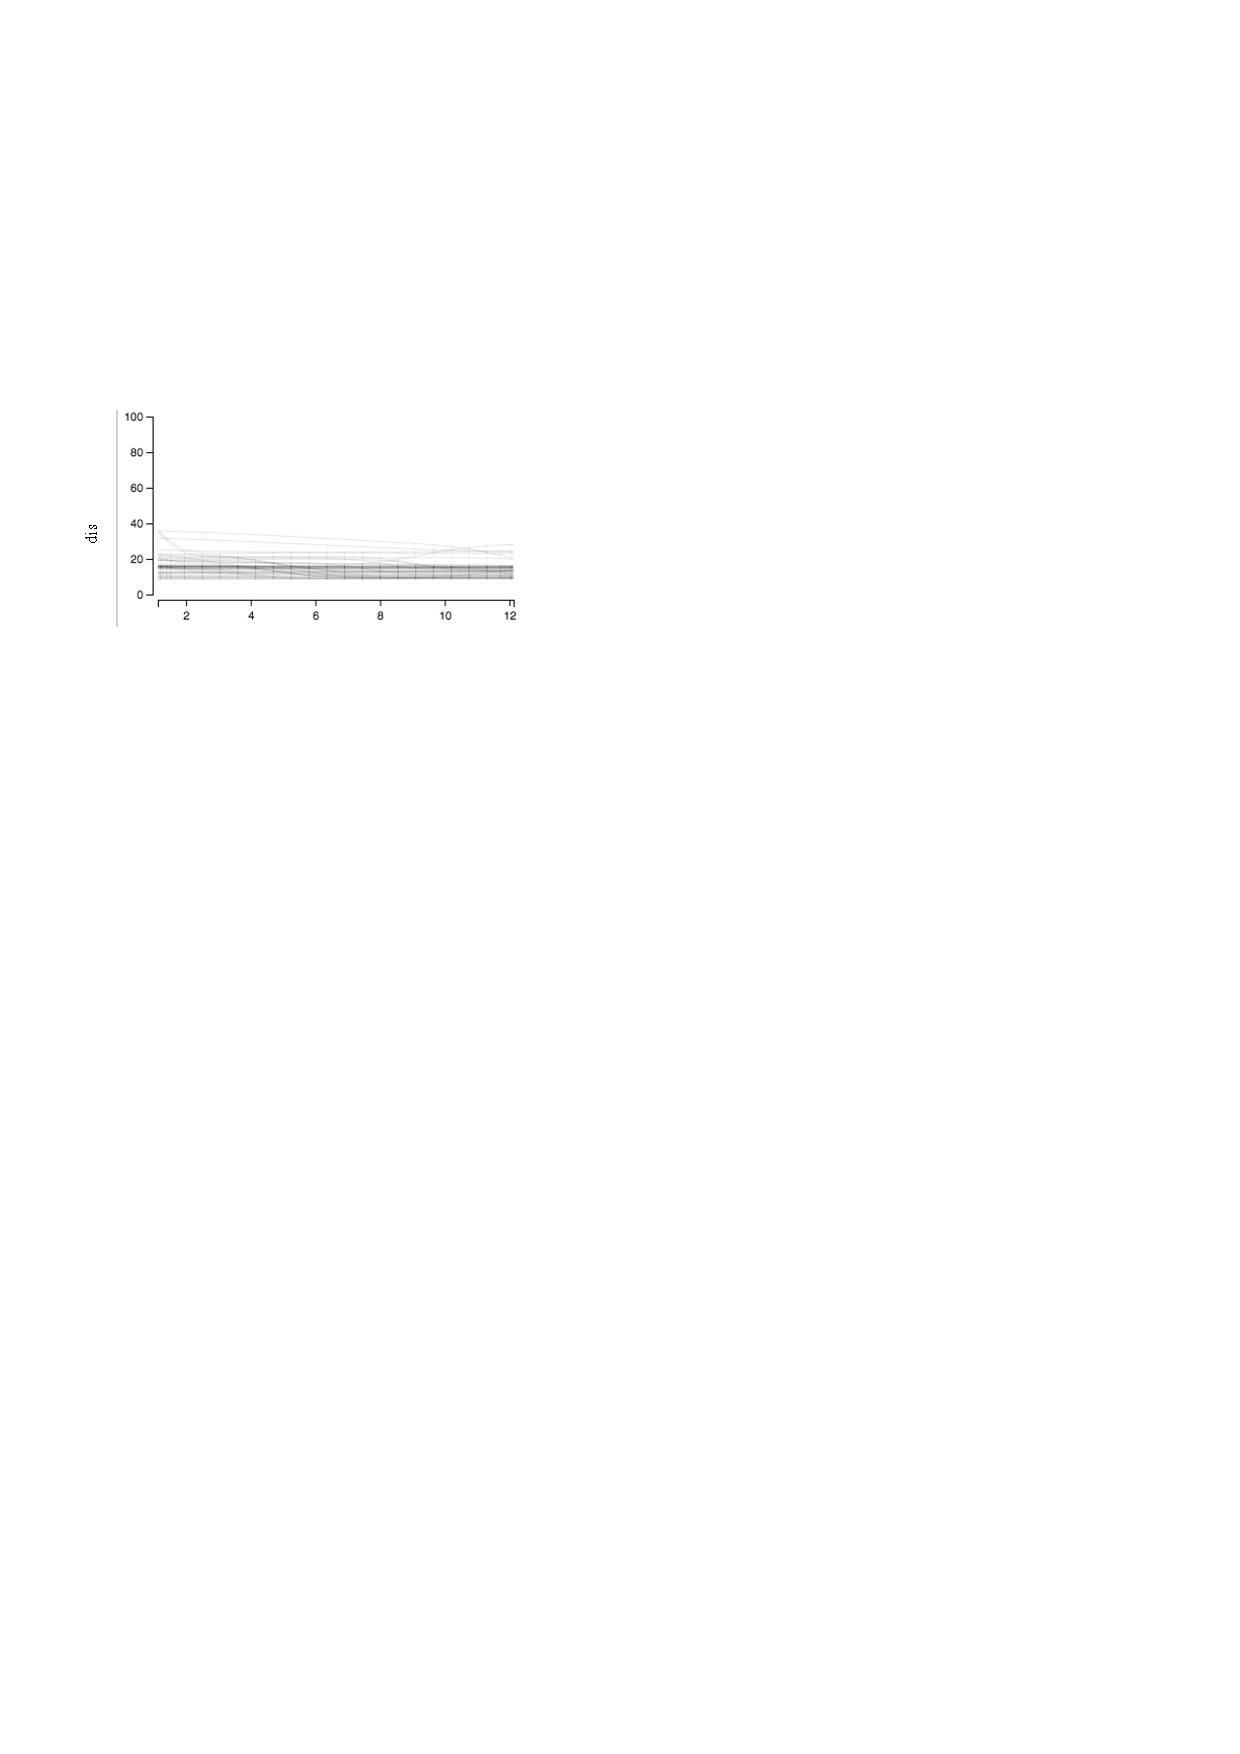
\includegraphics[width=0.1\textwidth]{nn5x3_8.pdf}
  &
    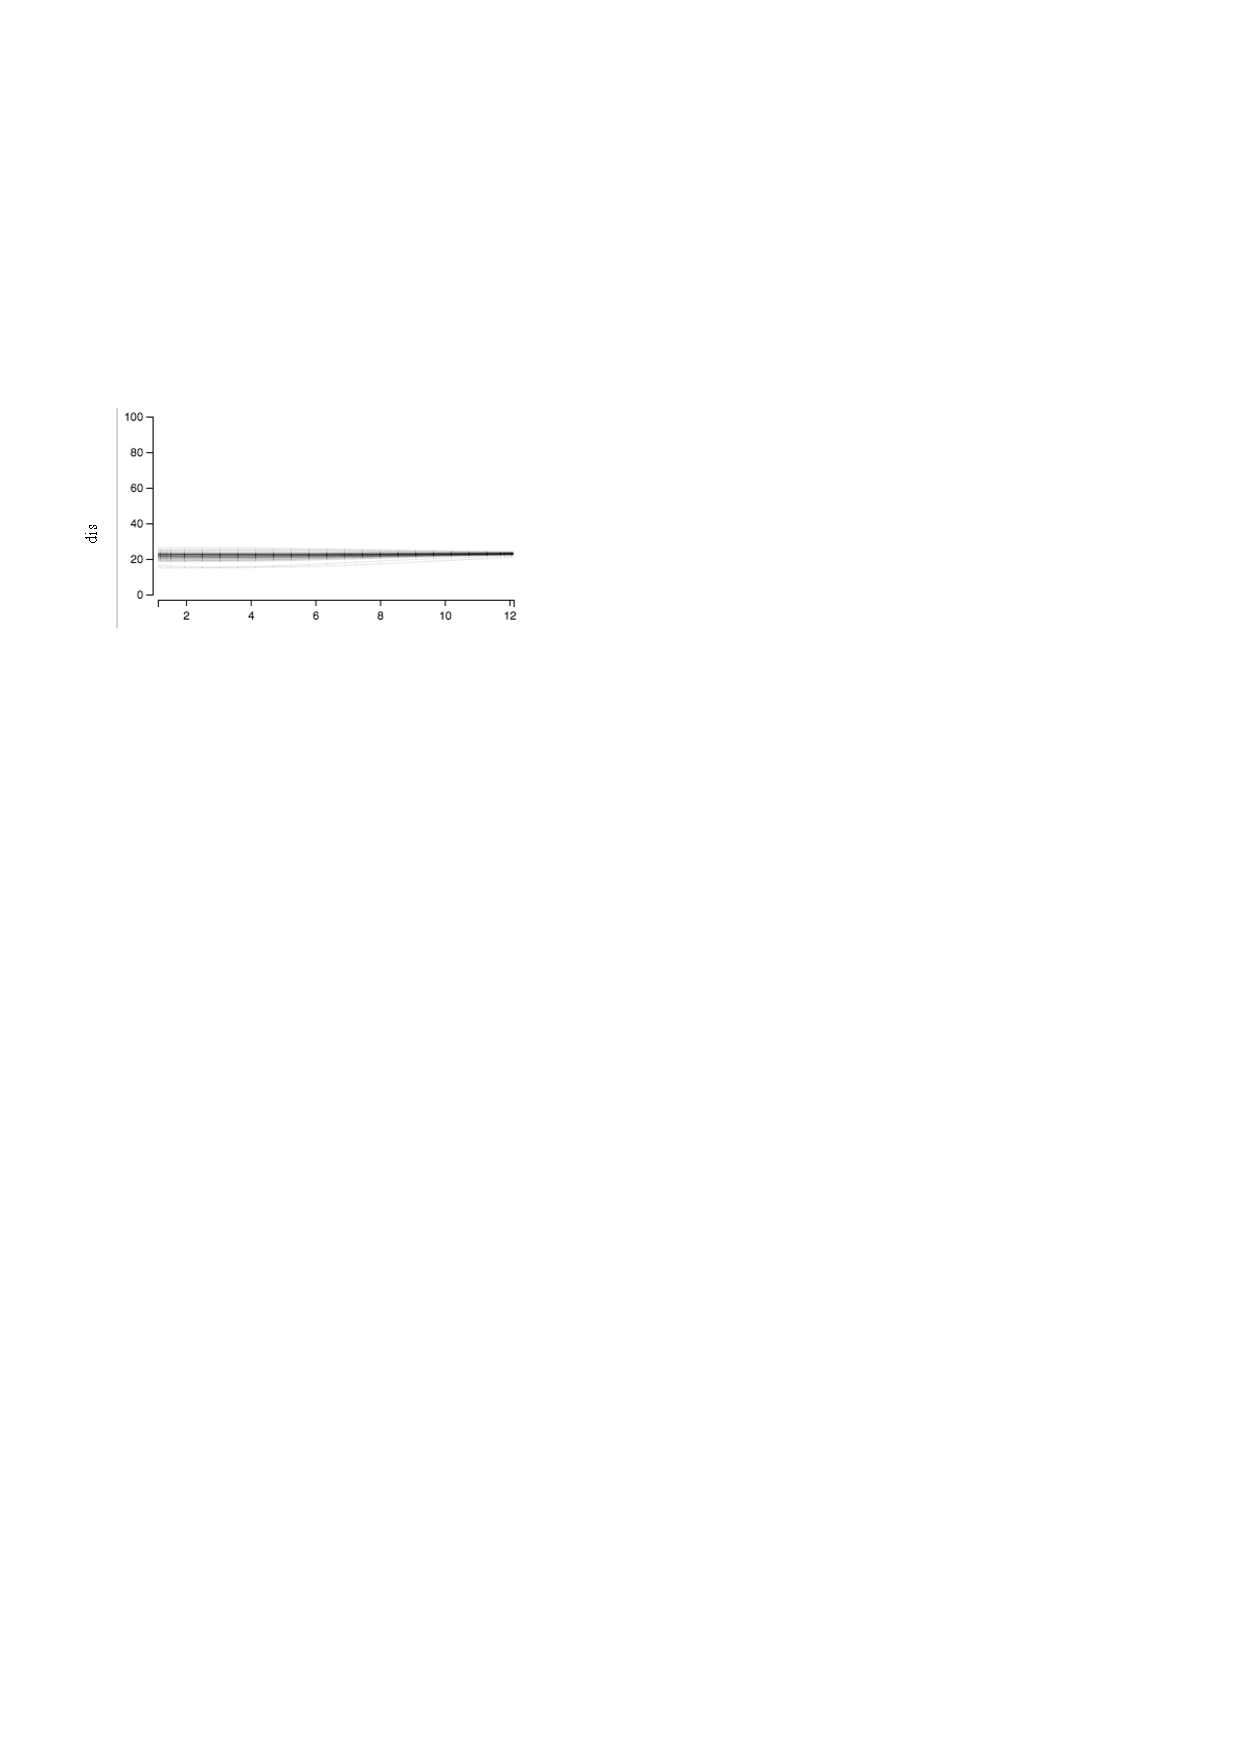
\includegraphics[width=0.1\textwidth]{svmr_8.pdf}
  \\
  \hline \\
  Accessibility to radial highways &
    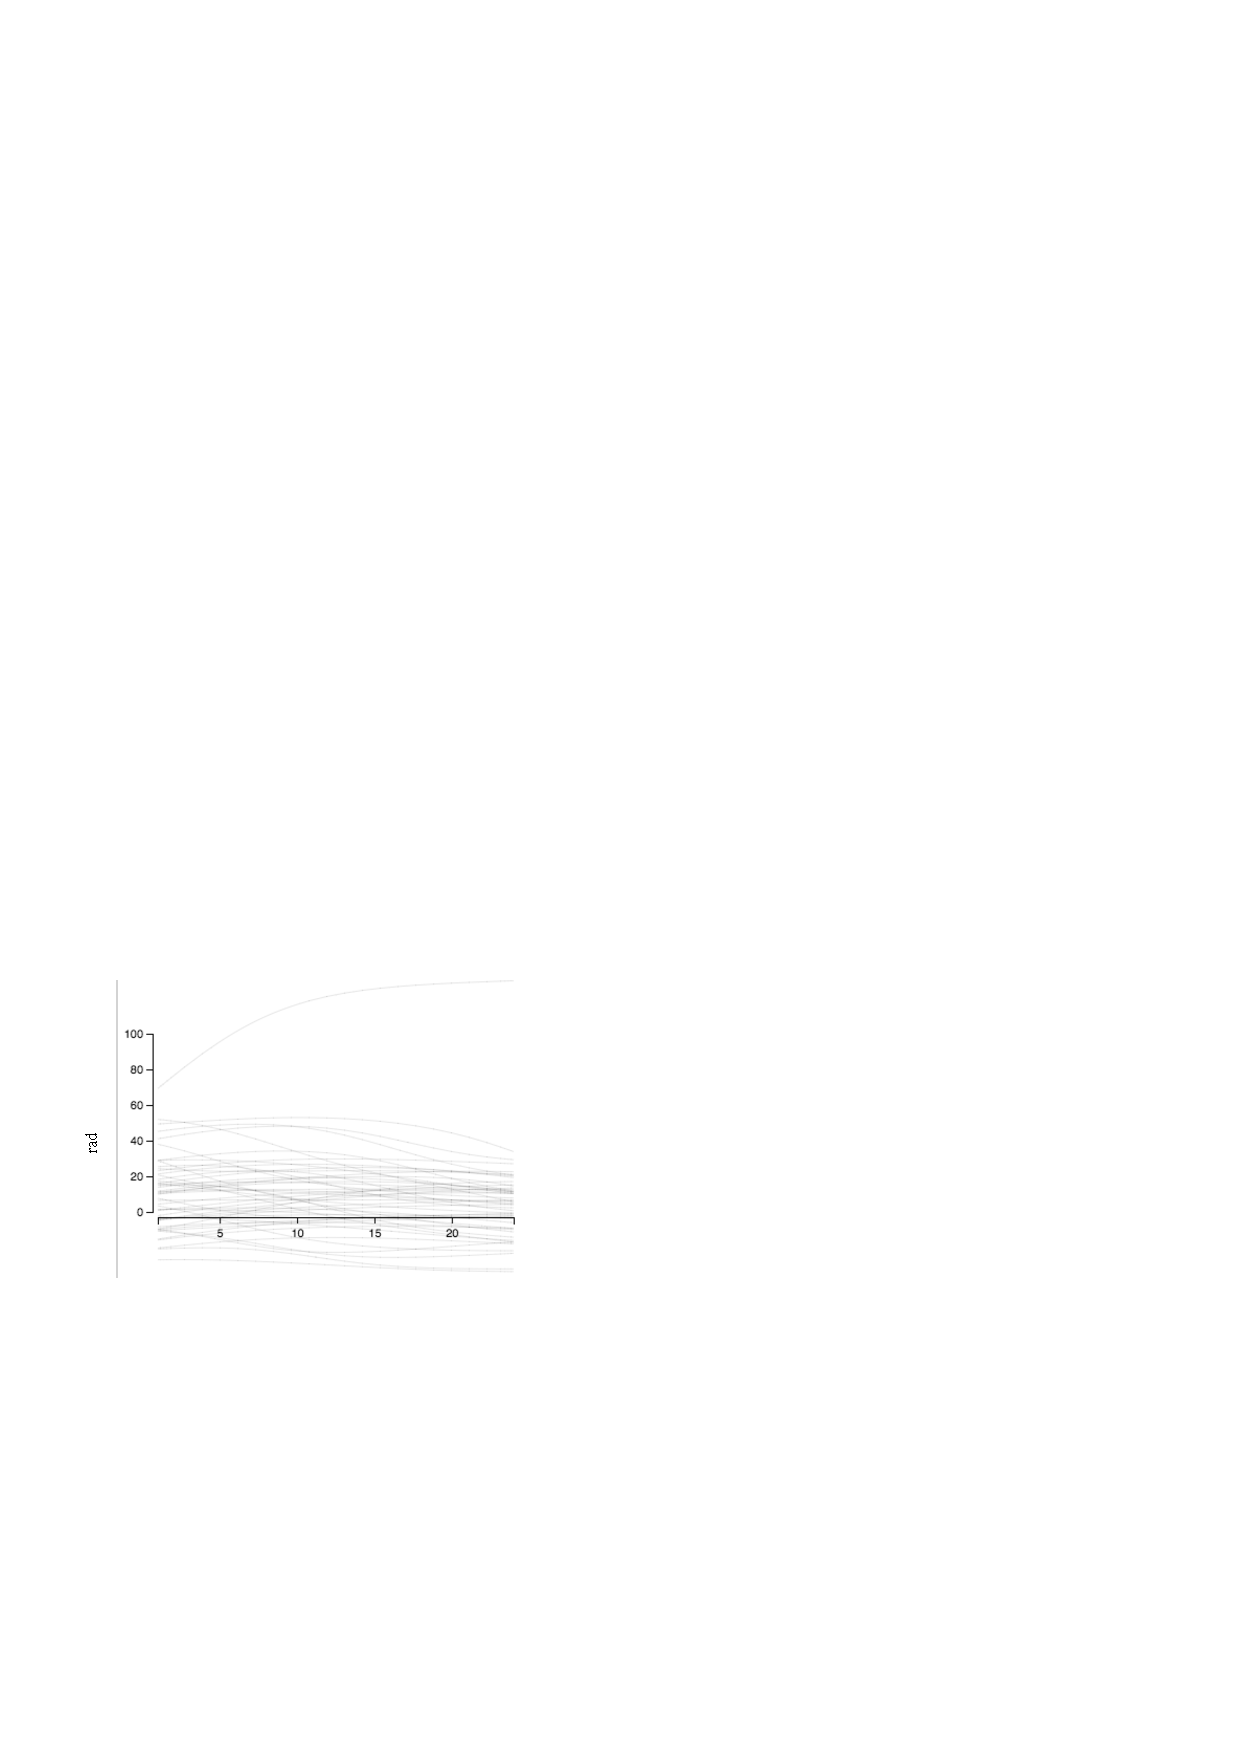
\includegraphics[width=0.1\textwidth]{nn26_9.pdf}
  &
    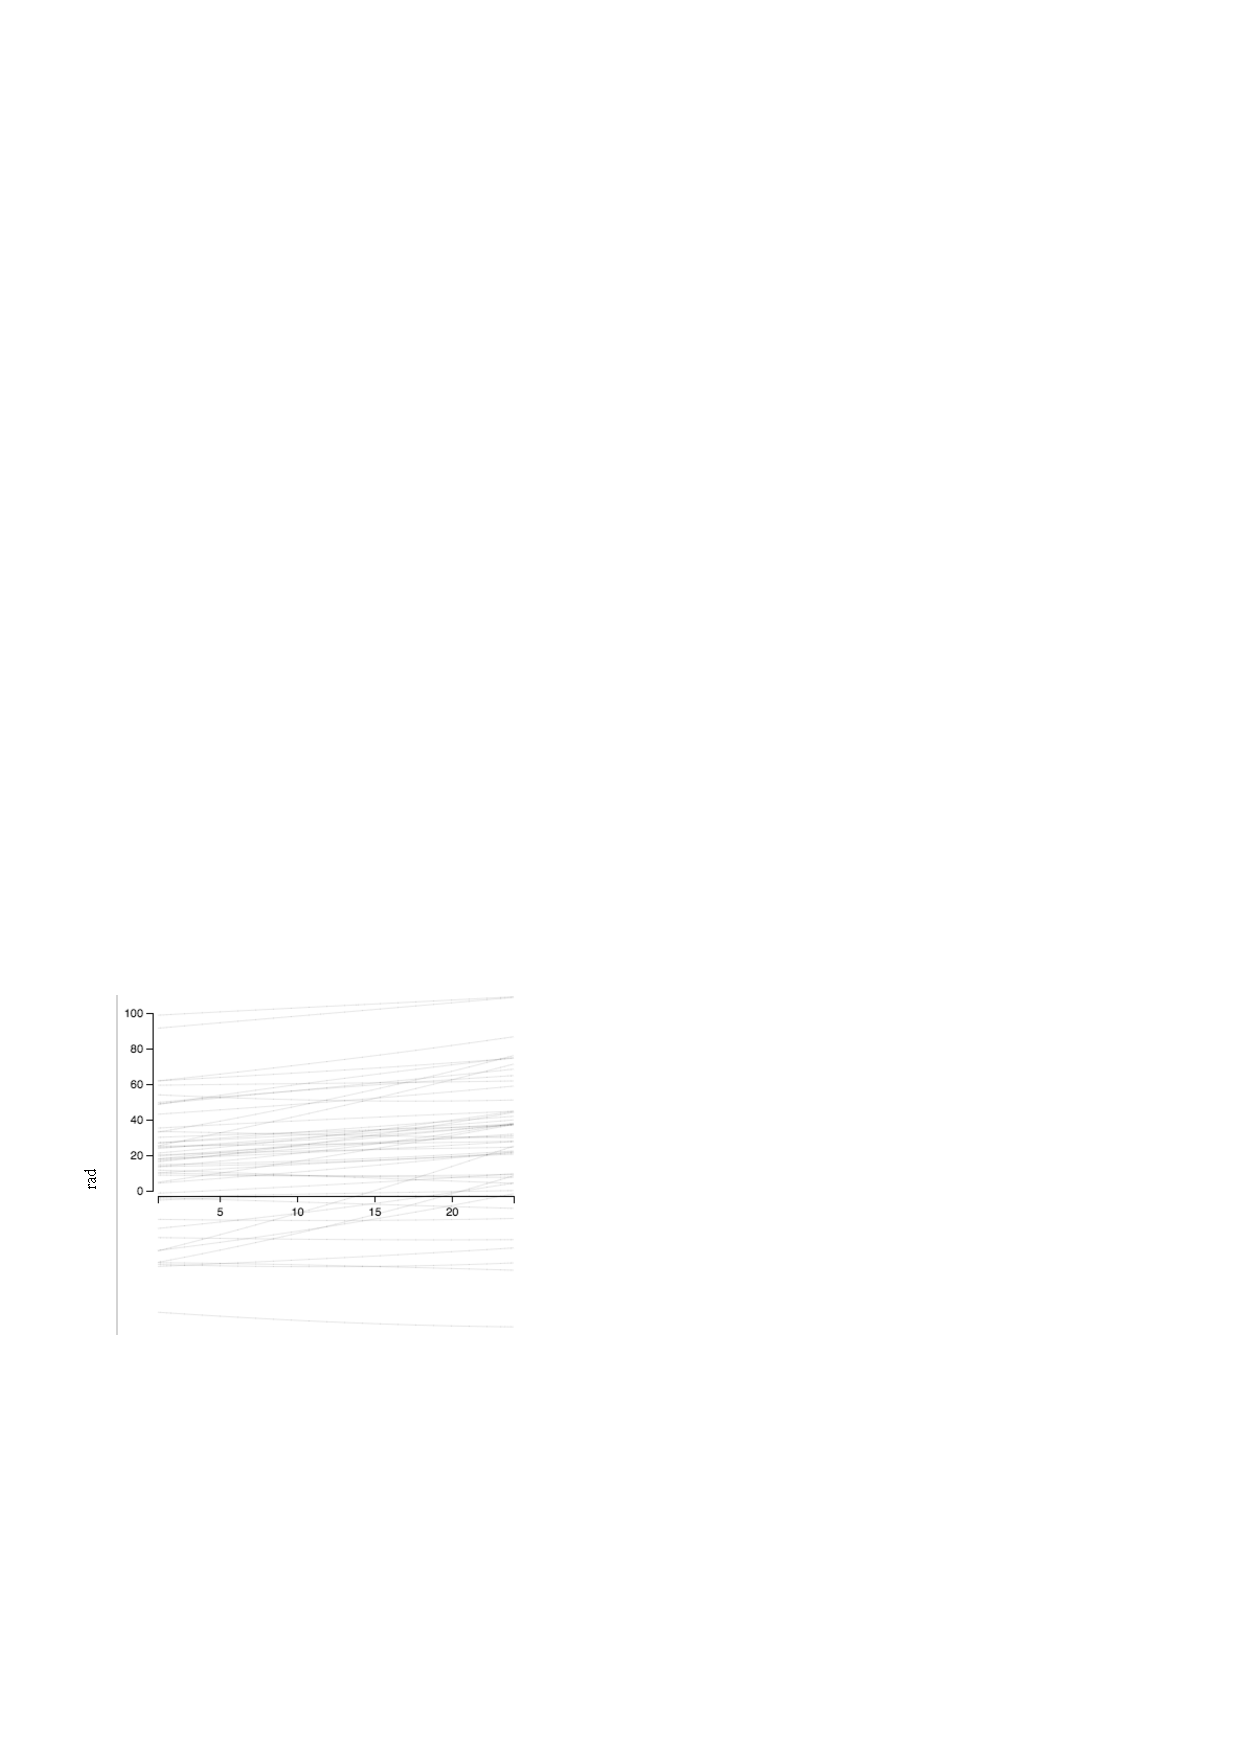
\includegraphics[width=0.1\textwidth]{svmp_9.pdf}
  &
    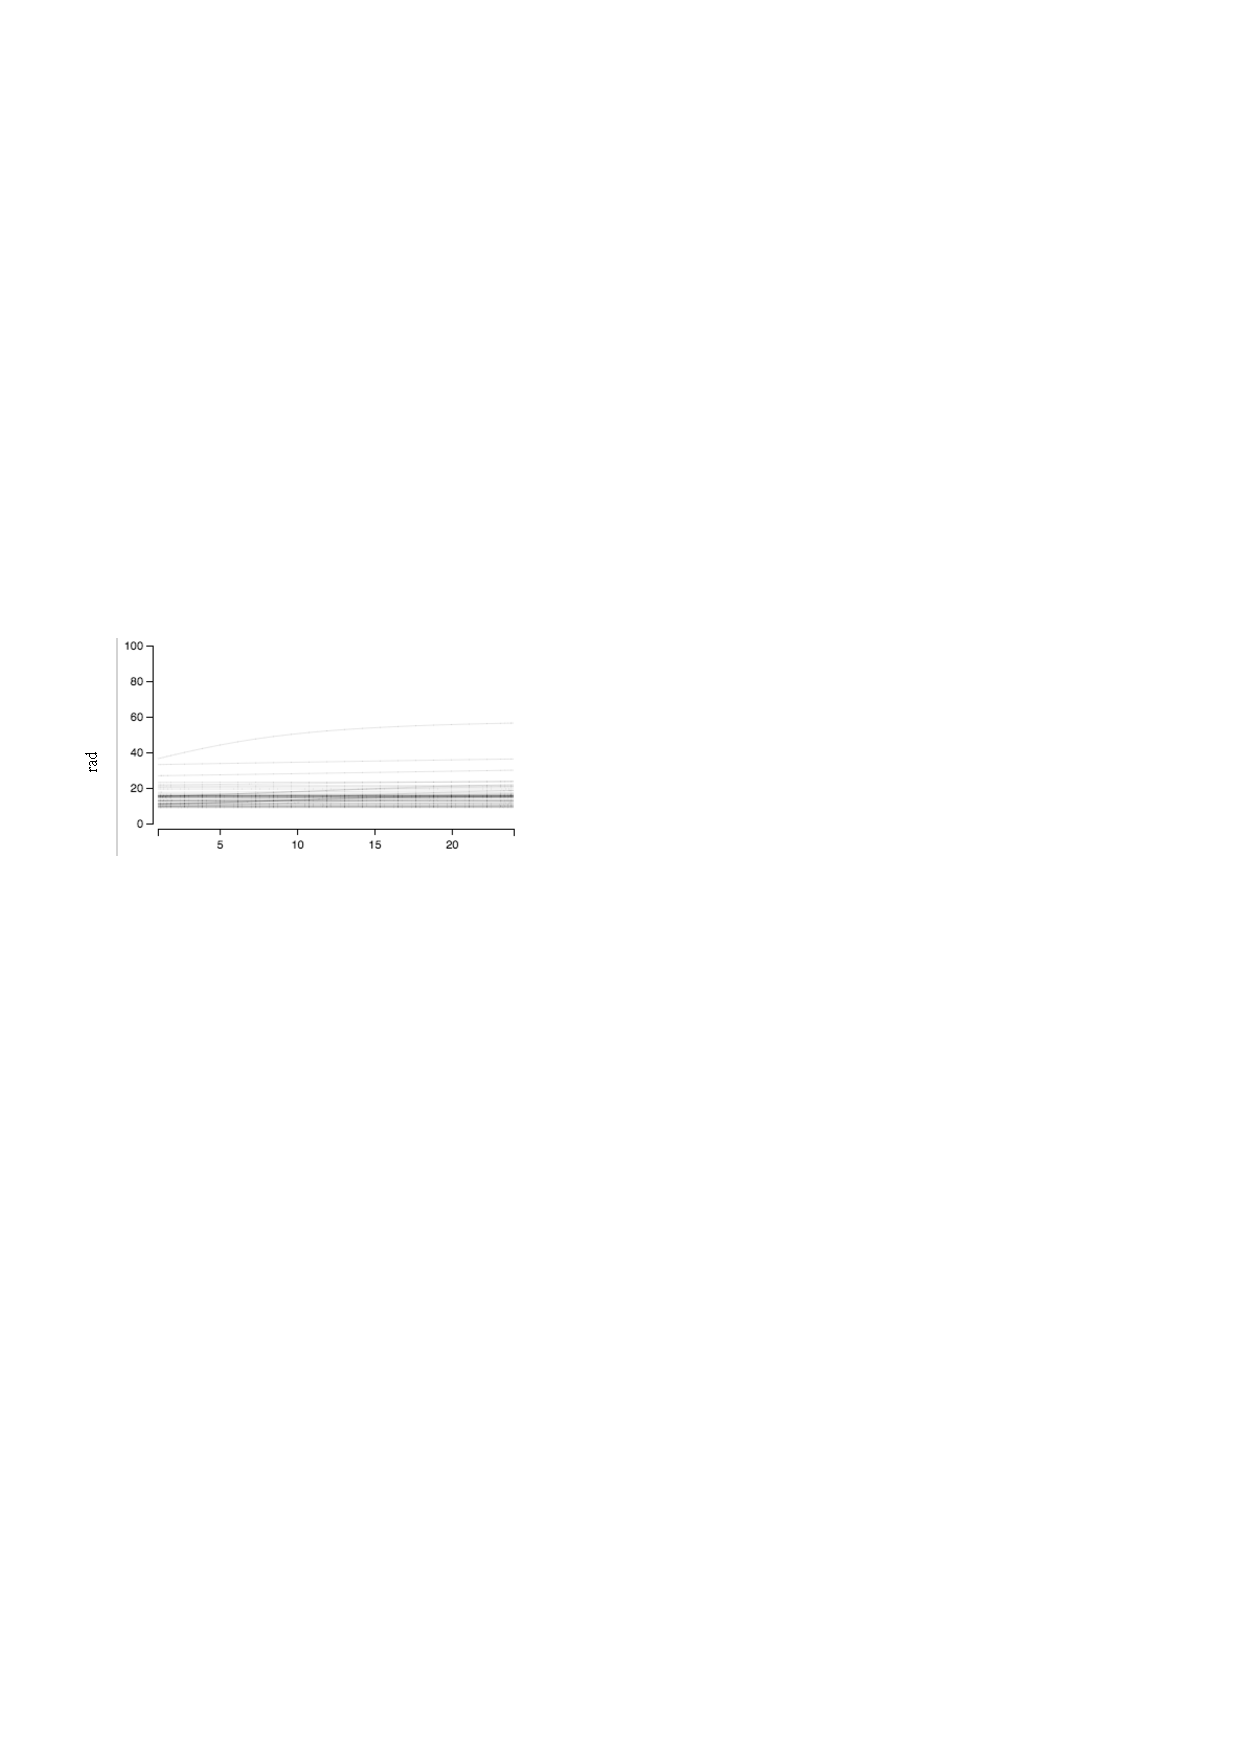
\includegraphics[width=0.1\textwidth]{nn5x3_9.pdf}
  &
    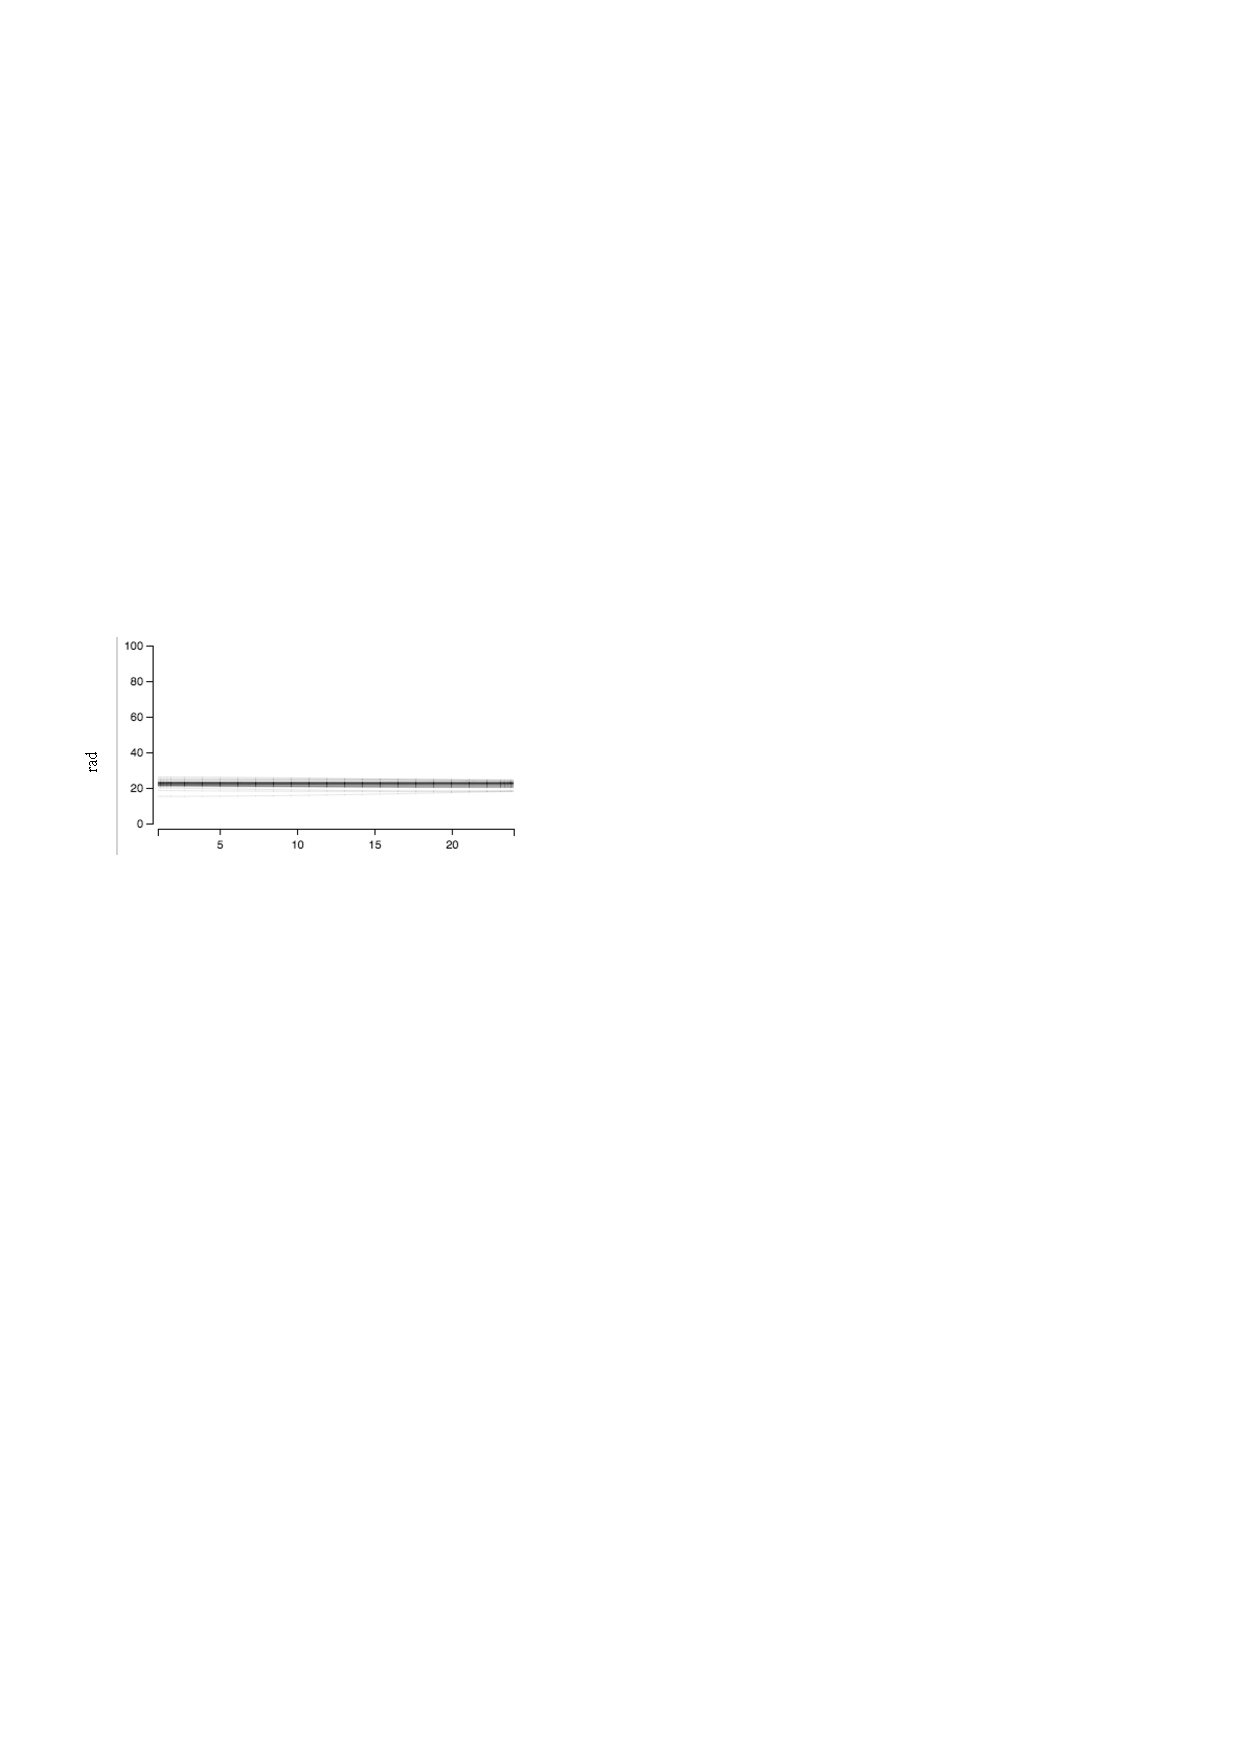
\includegraphics[width=0.1\textwidth]{svmr_9.pdf}
  \\
  \hline \\
  Property-tax rate &
    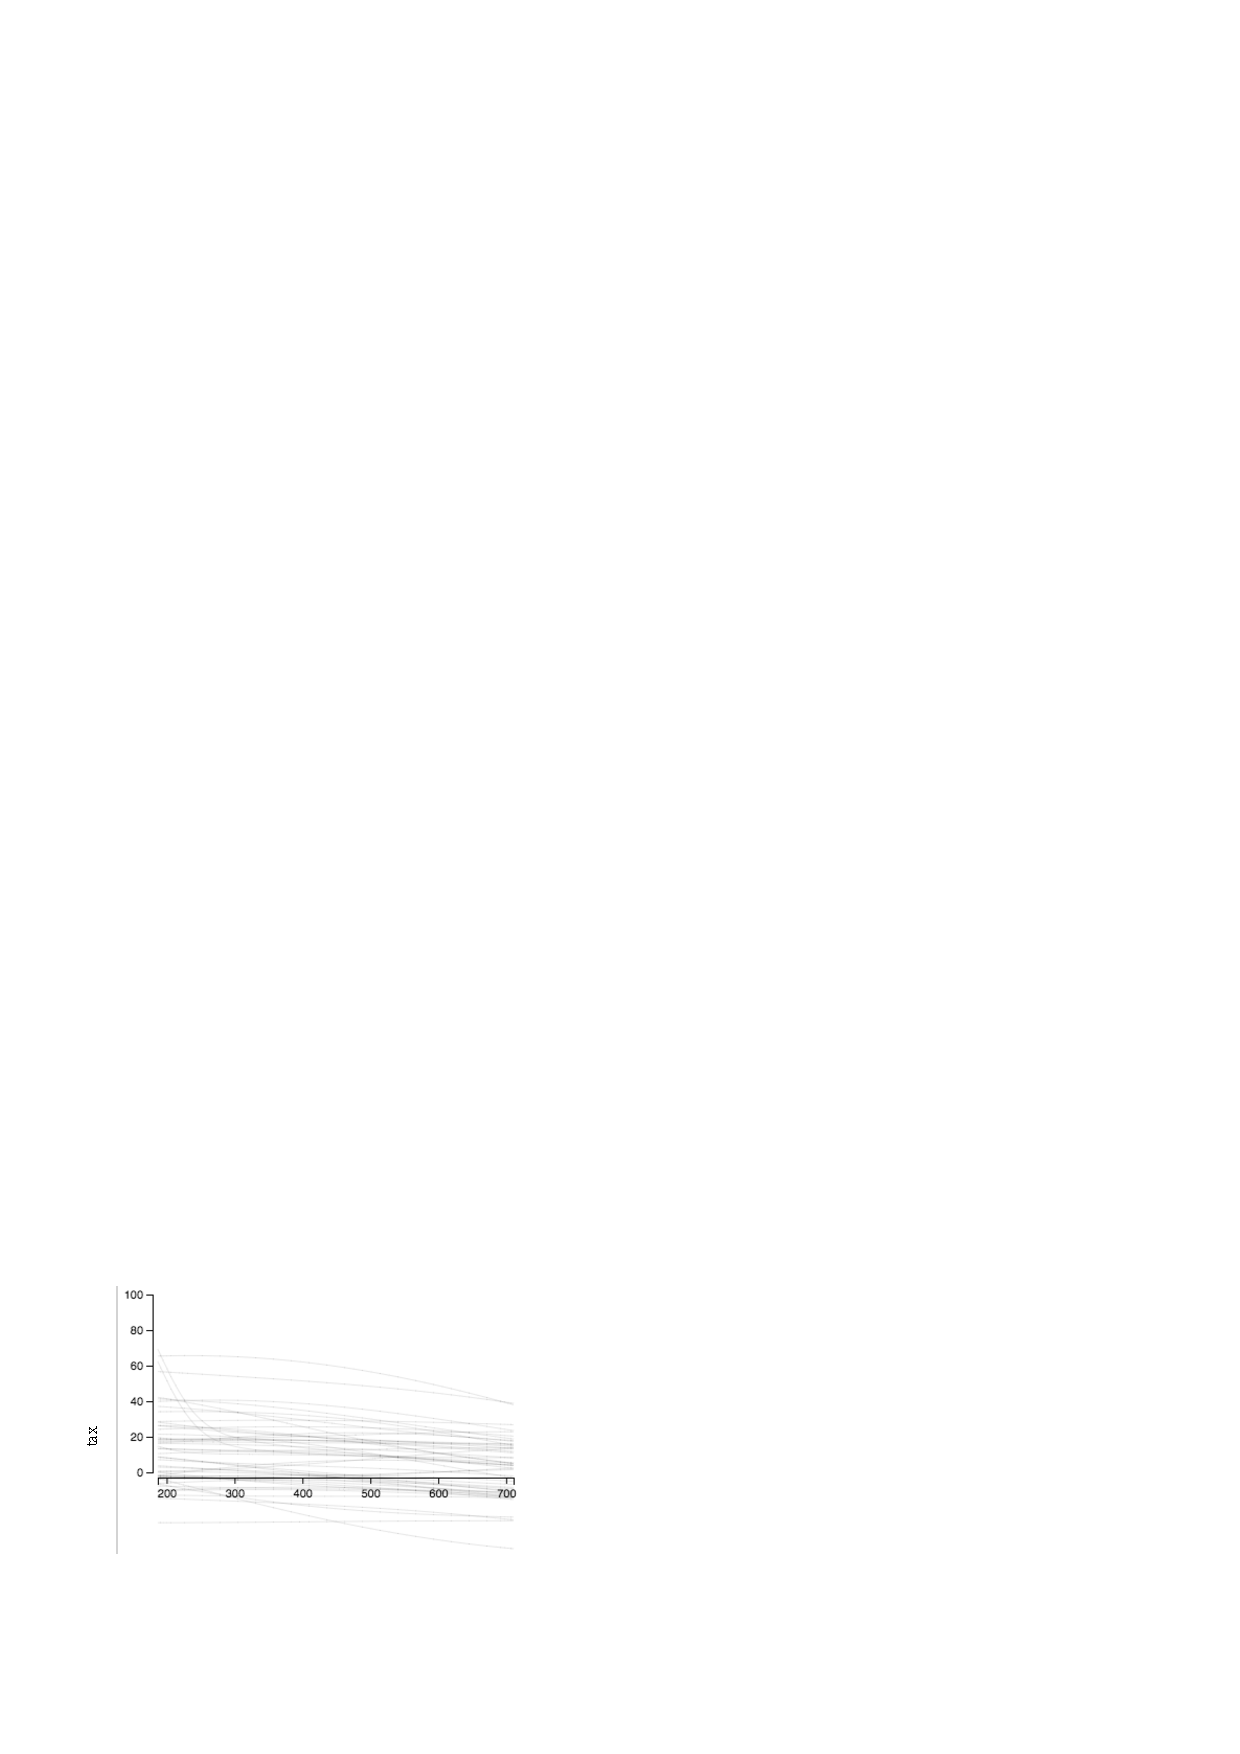
\includegraphics[width=0.1\textwidth]{nn26_10.pdf}
  &
    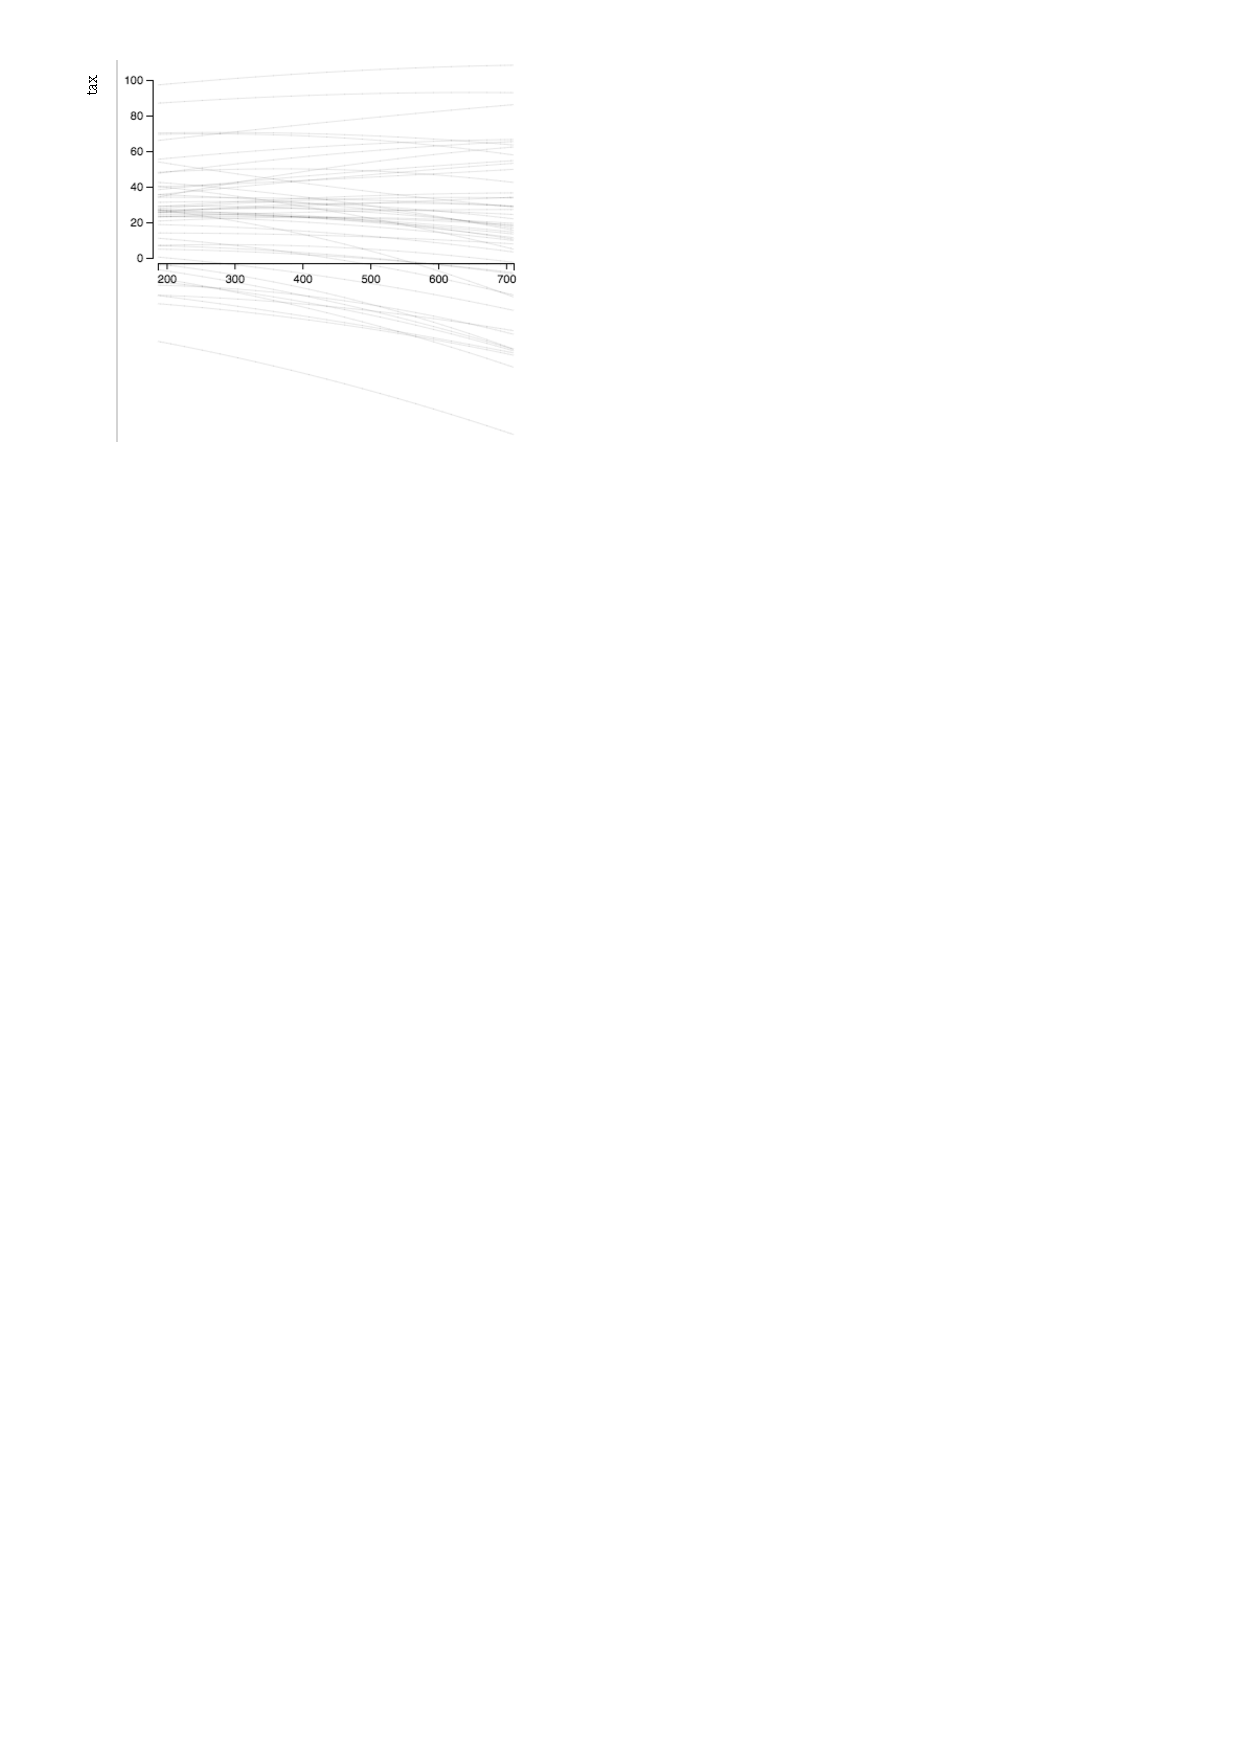
\includegraphics[width=0.1\textwidth]{svmp_10.pdf}
  &
    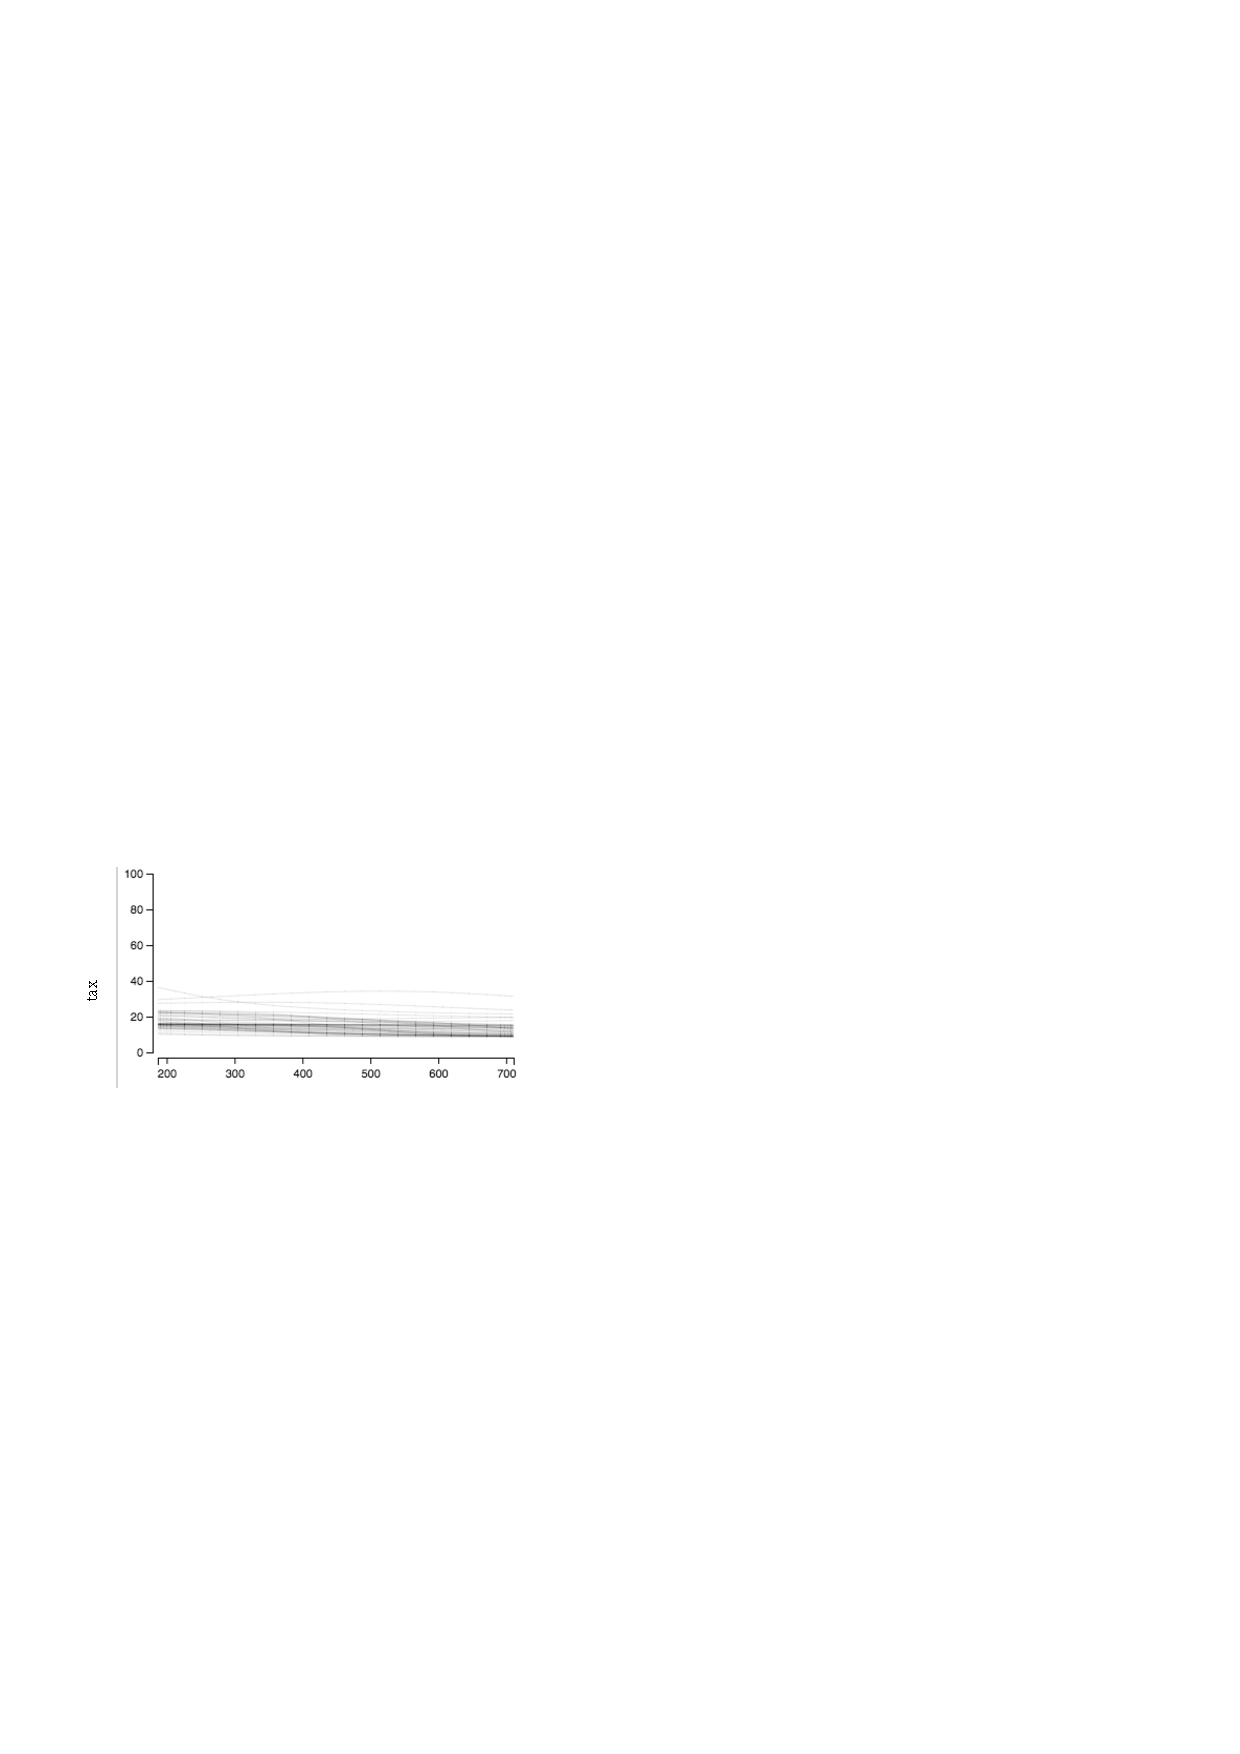
\includegraphics[width=0.1\textwidth]{nn5x3_10.pdf}
  &
    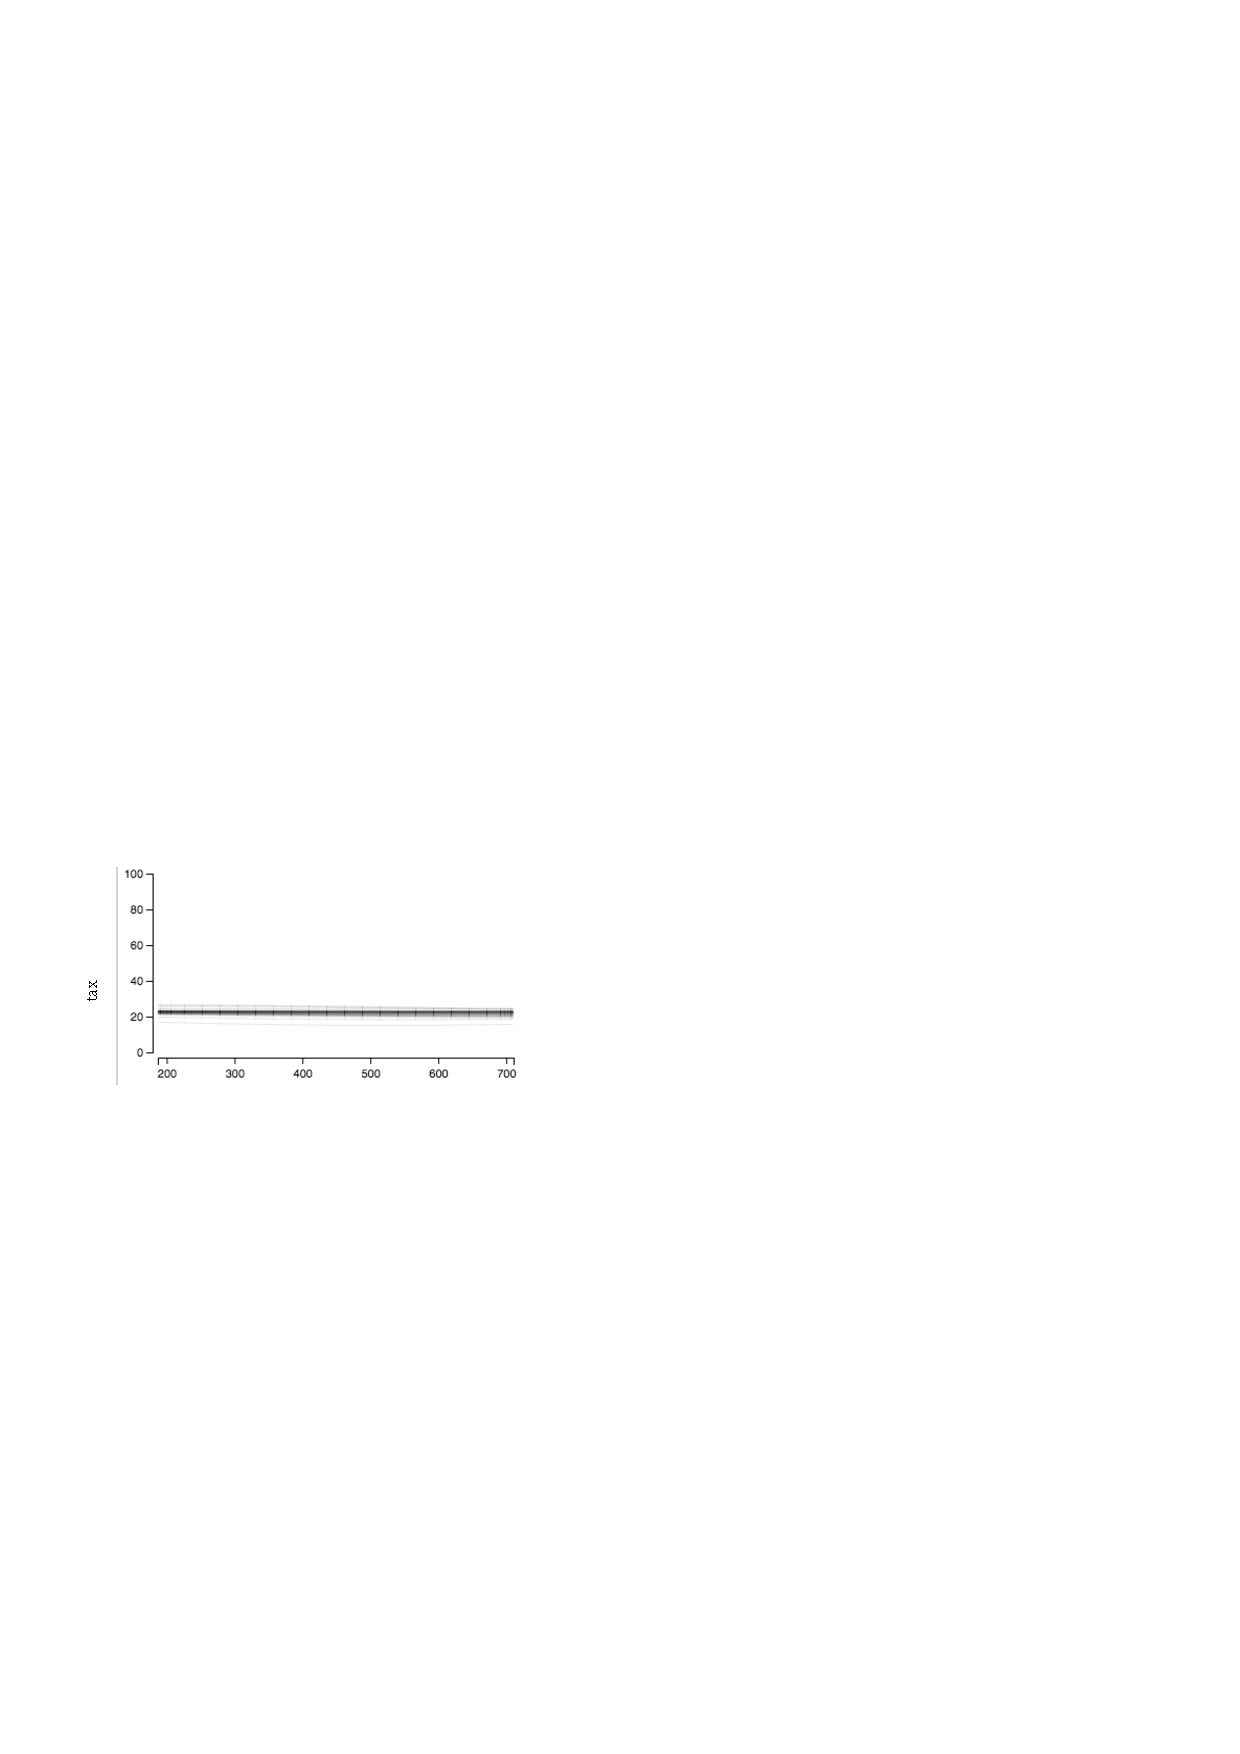
\includegraphics[width=0.1\textwidth]{svmr_10.pdf}
  \\
  \hline \\
  Pupil-teacher ratio &
    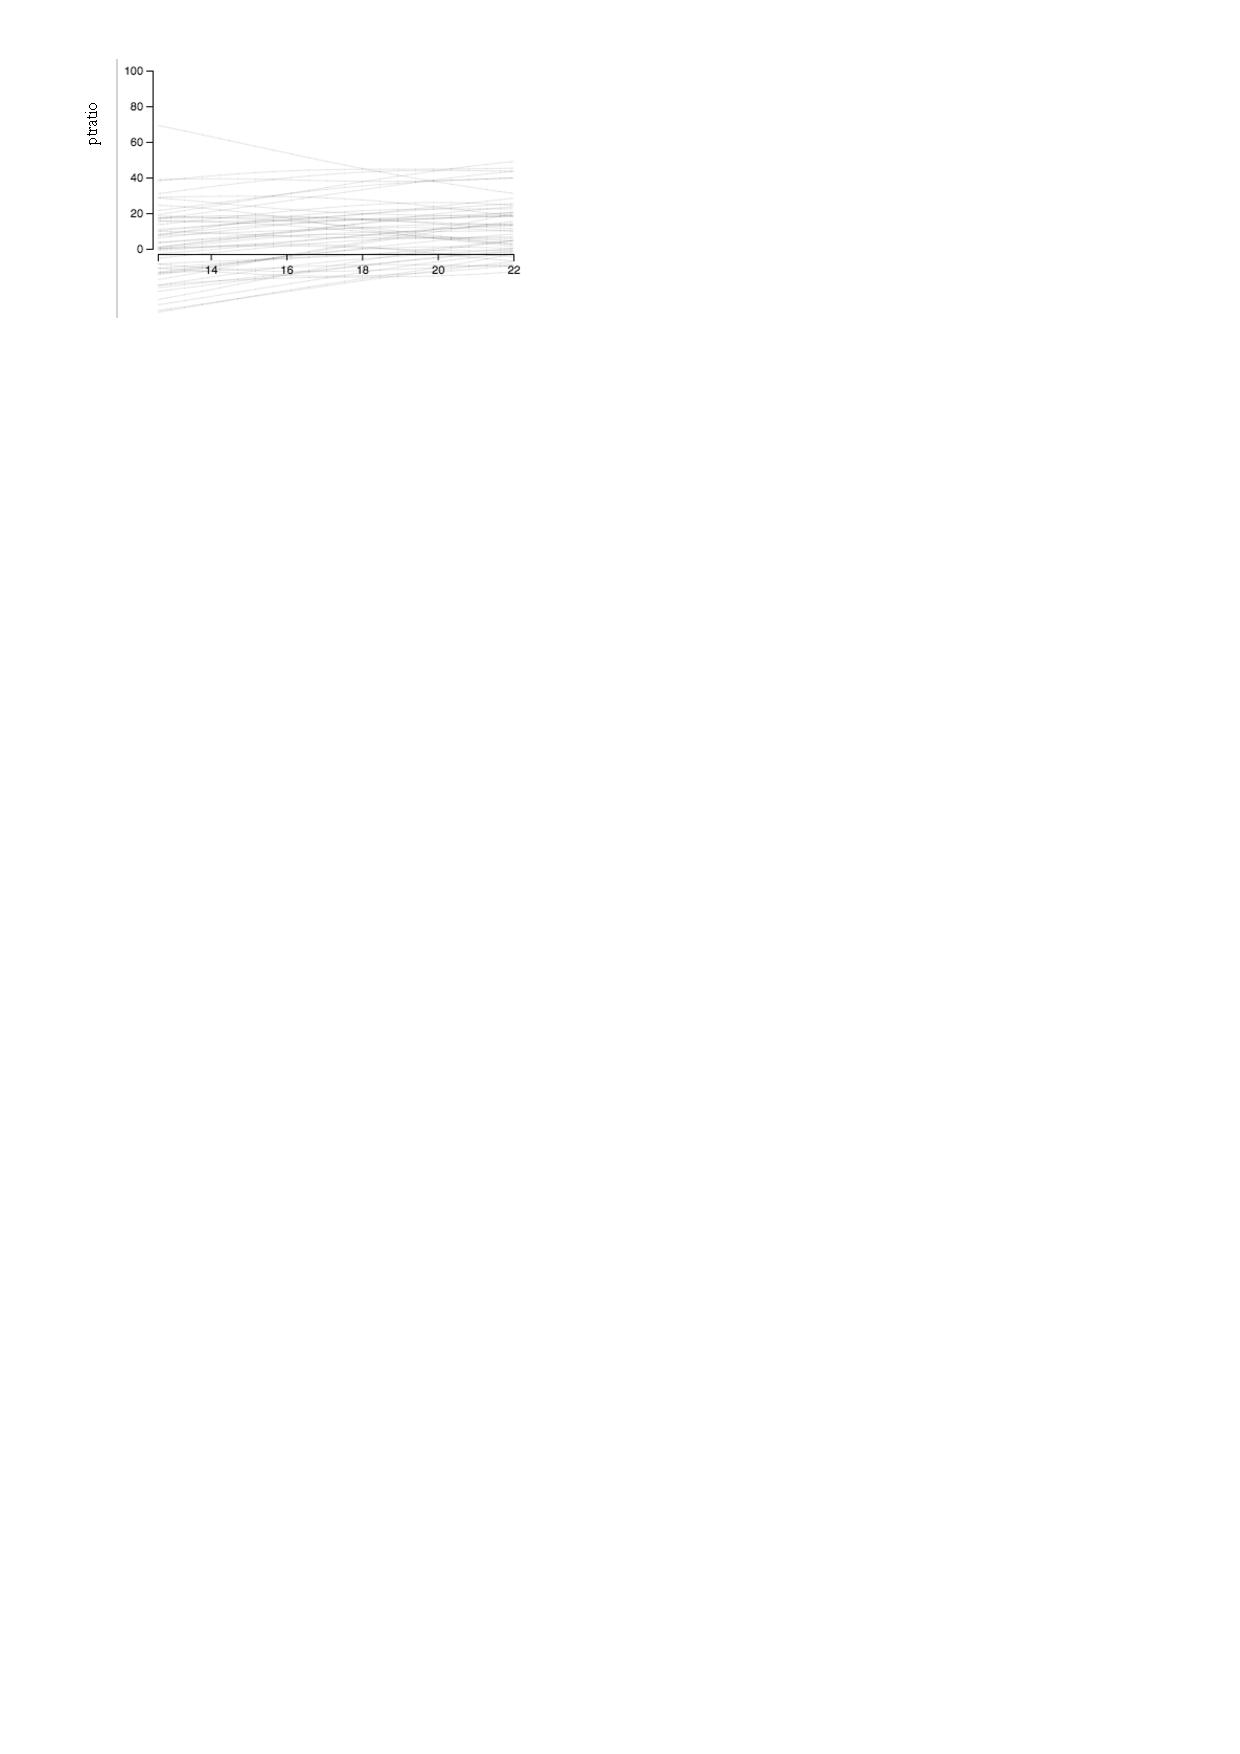
\includegraphics[width=0.1\textwidth]{nn26_11.pdf}
  &
    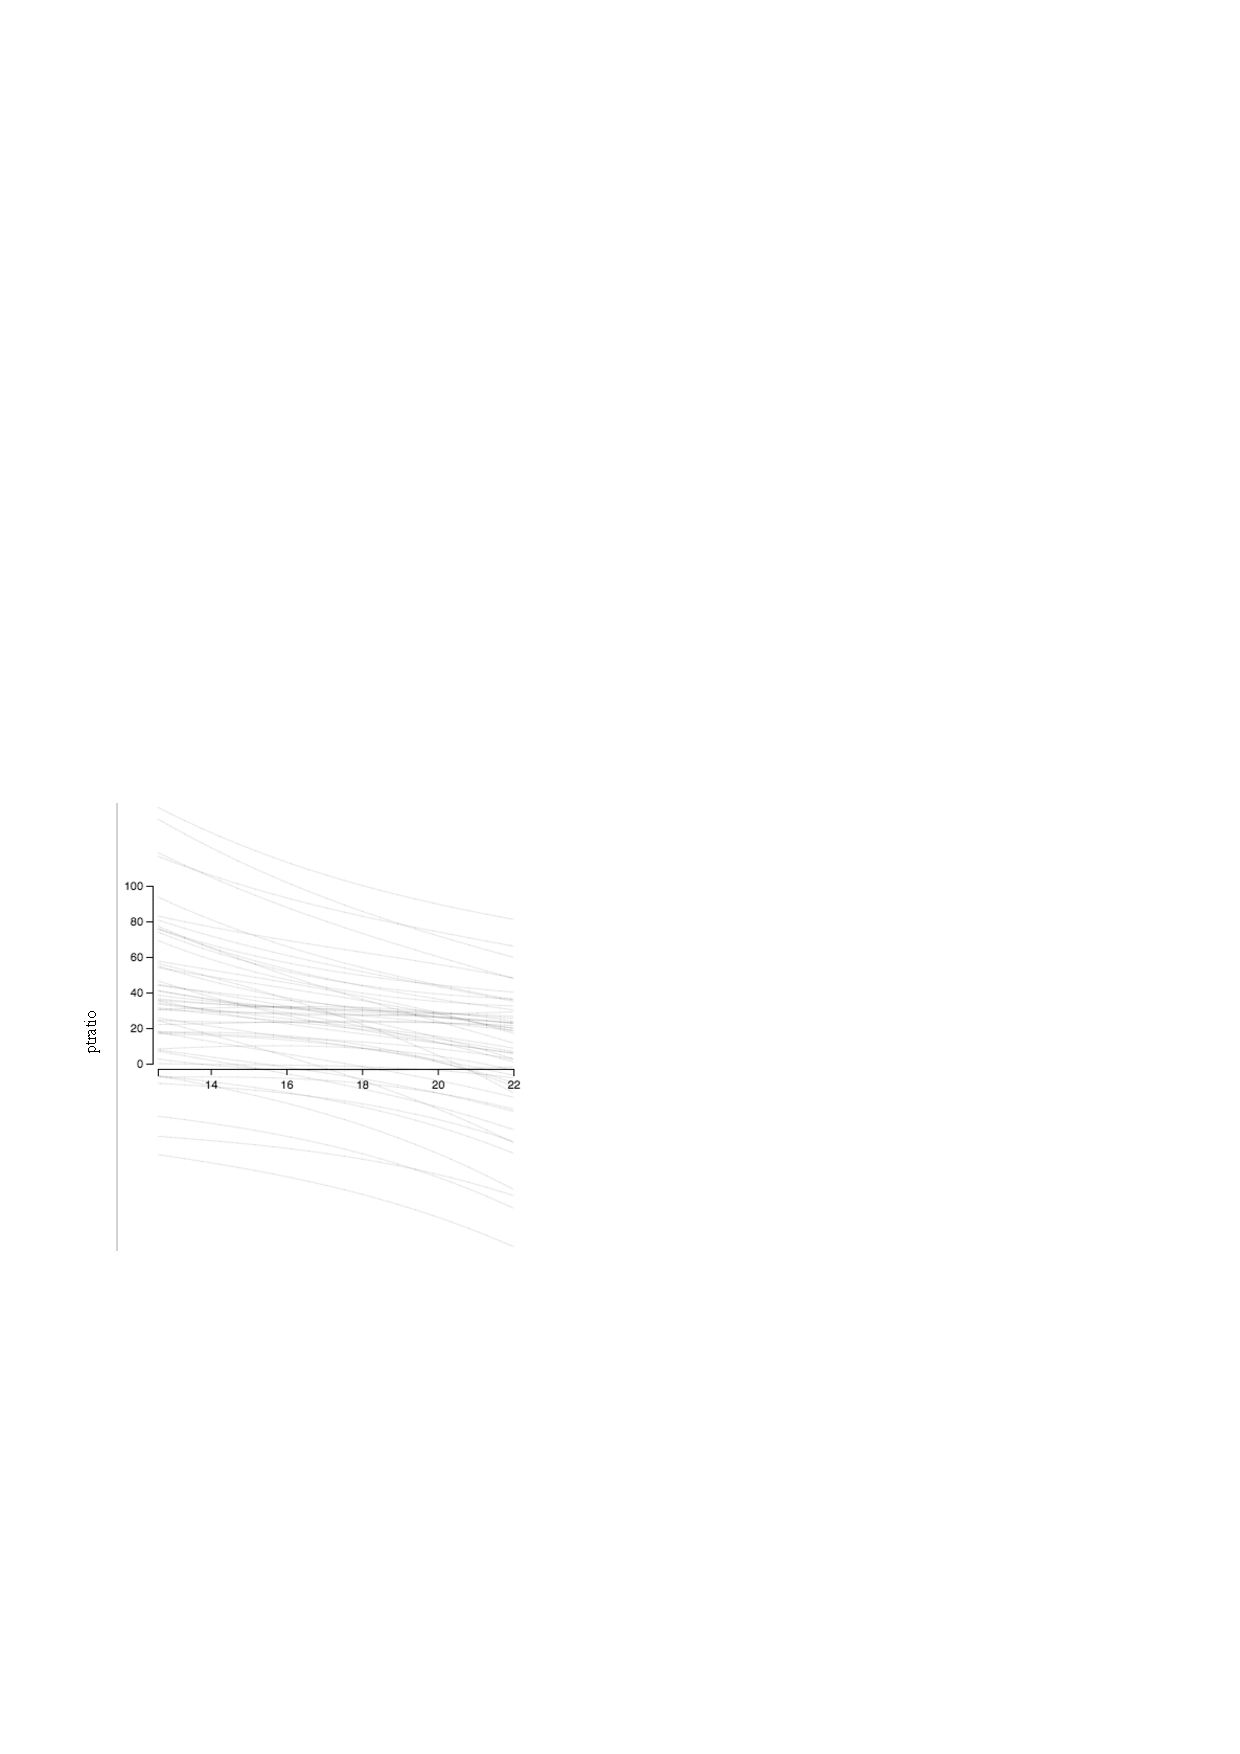
\includegraphics[width=0.1\textwidth]{svmp_11.pdf}
  &
    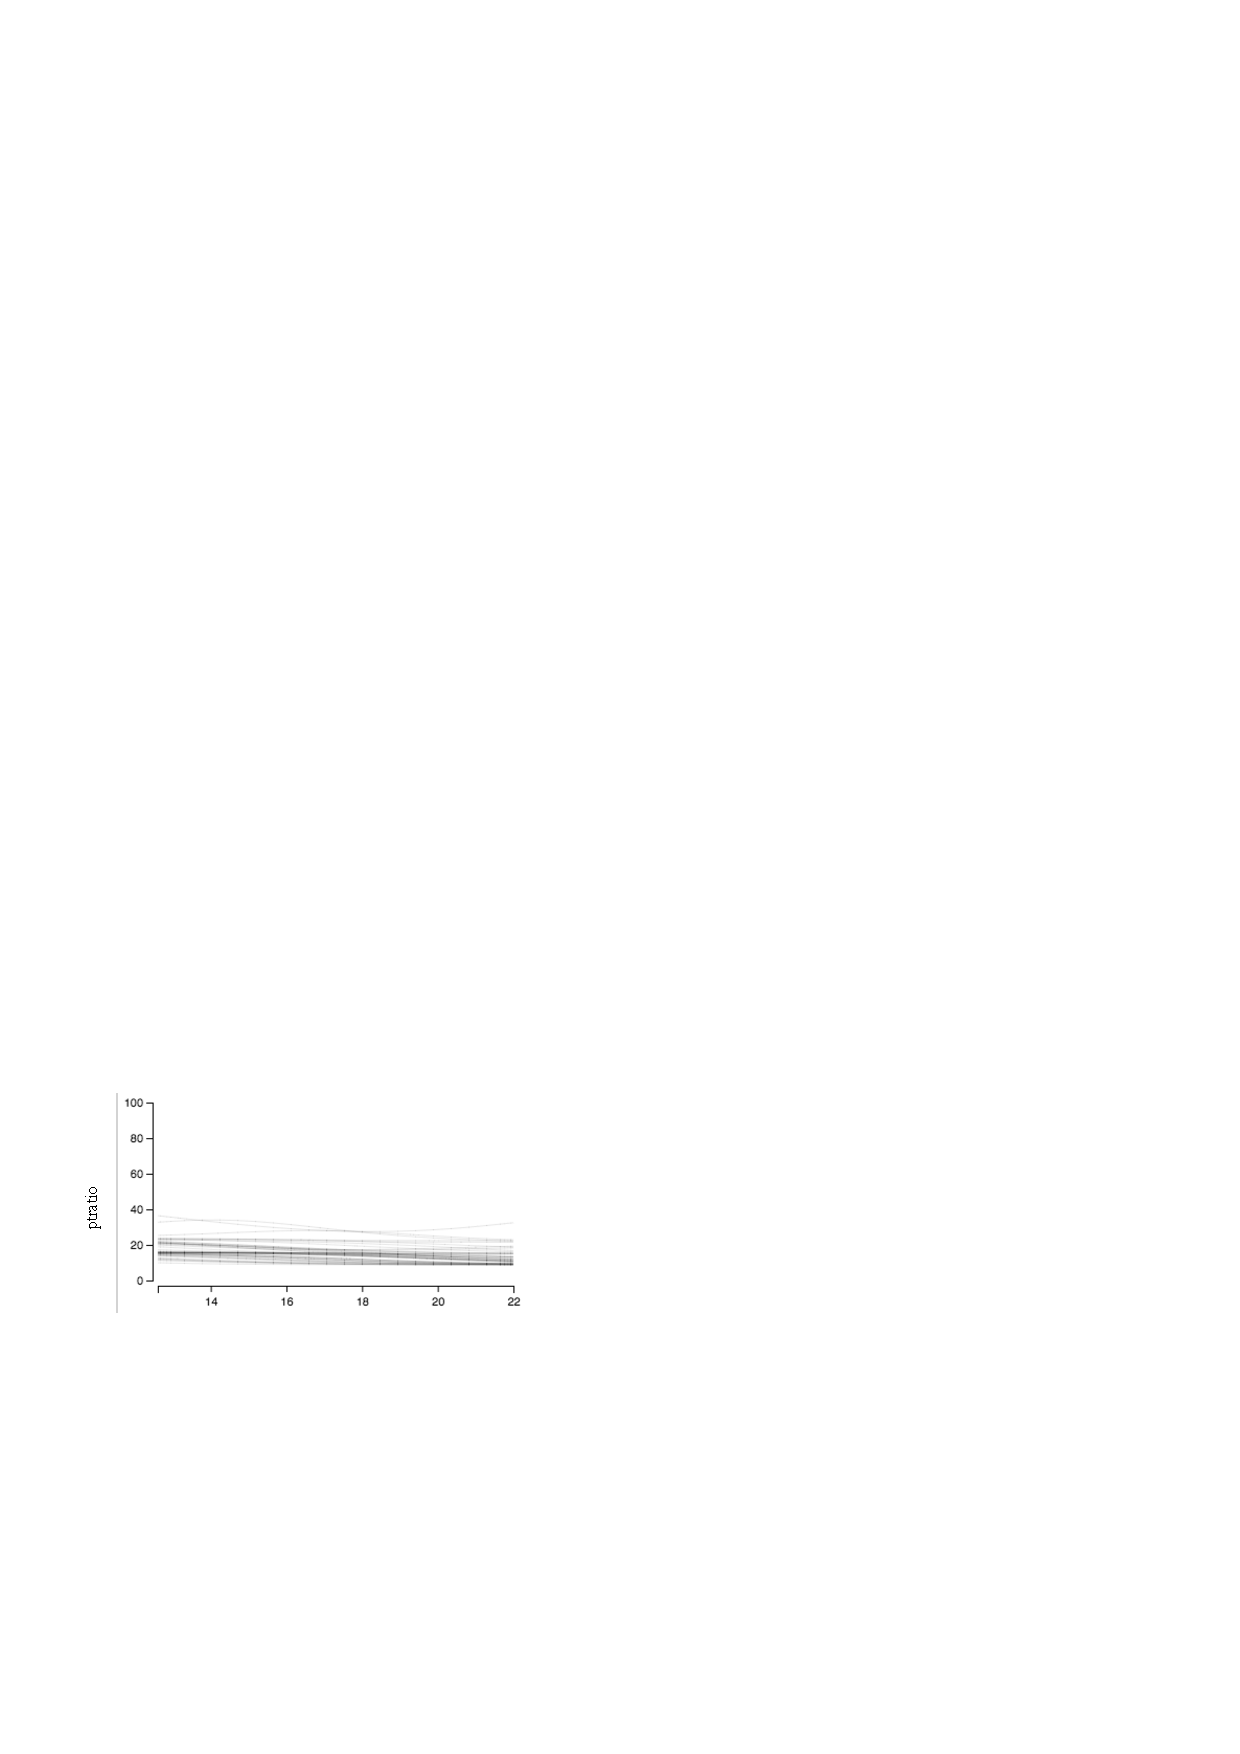
\includegraphics[width=0.1\textwidth]{nn5x3_11.pdf}
  &
    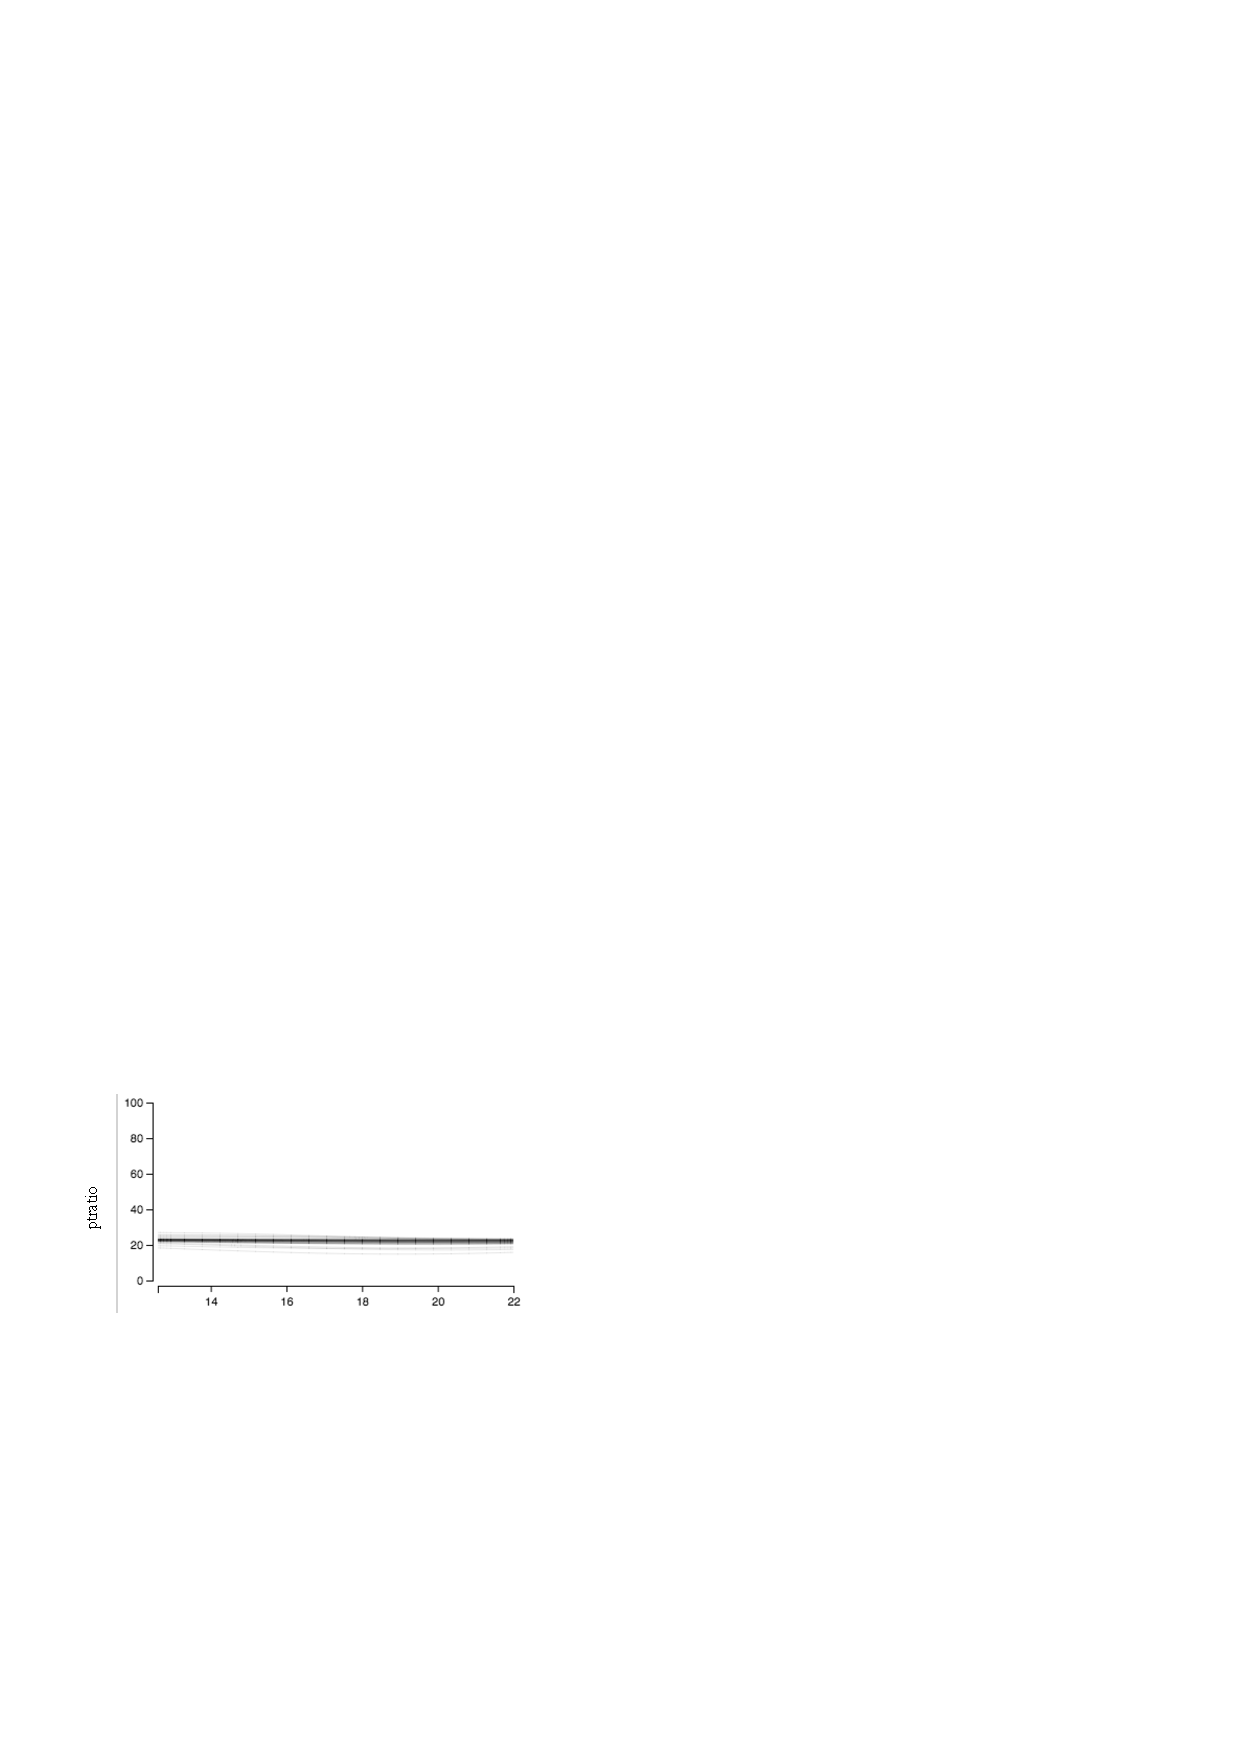
\includegraphics[width=0.1\textwidth]{svmr_11.pdf}
  \\
  \hline \\
  Proportion of blacks &
    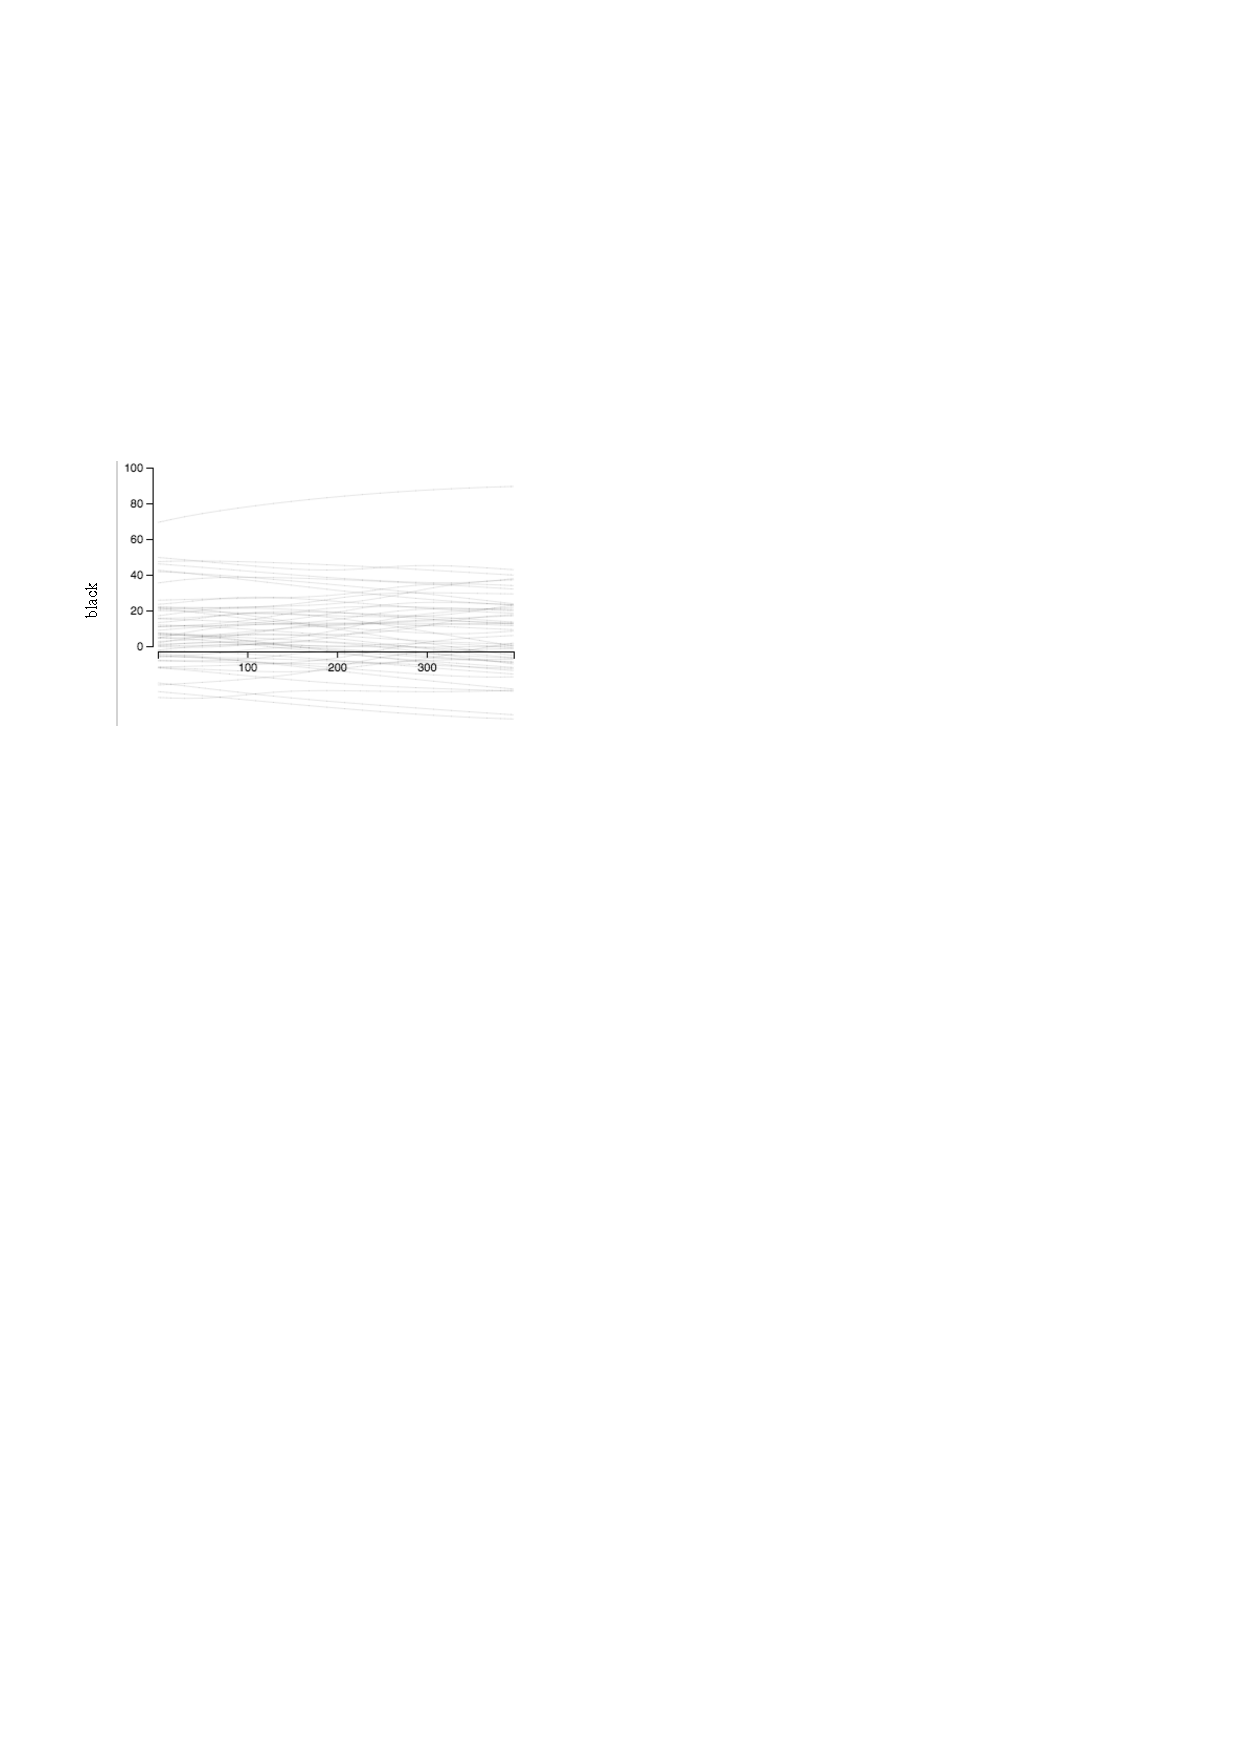
\includegraphics[width=0.1\textwidth]{nn26_12.pdf}
  &
    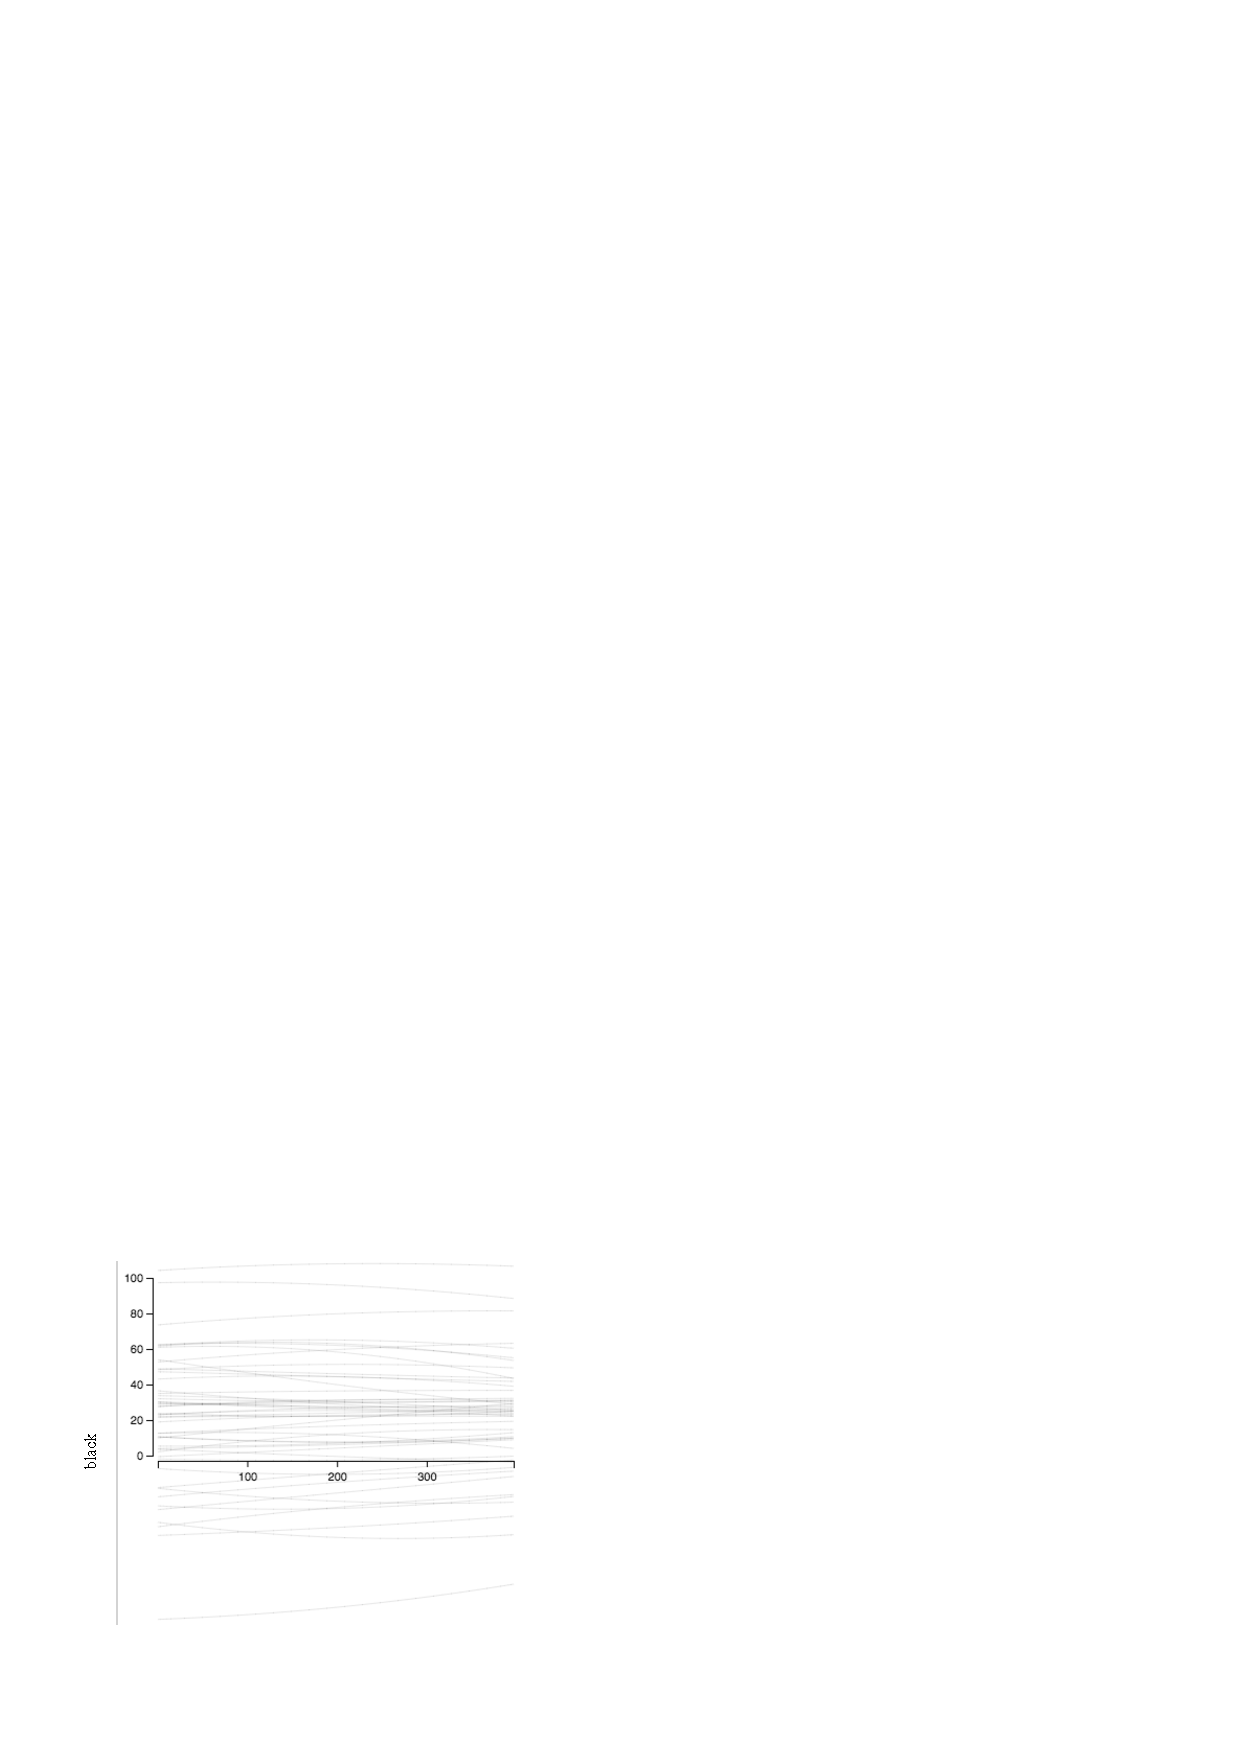
\includegraphics[width=0.1\textwidth]{svmp_12.pdf}
  &
    \includegraphics[width=0.1\textwidth]{nn5x3_12.pdf}
  &
    \includegraphics[width=0.1\textwidth]{svmr_12.pdf}
  \\
  \hline \\
  \% lower income status of the population &
    \includegraphics[width=0.1\textwidth]{nn26_13.pdf}
  &
    \includegraphics[width=0.1\textwidth]{svmp_13.pdf}
  &
    \includegraphics[width=0.1\textwidth]{nn5x3_13.pdf}
  &
    \includegraphics[width=0.1\textwidth]{svmr_13.pdf}
  \\
  \hline \\
\end{longtable}
\end{tiny}

